\documentclass[a4paper, 12pt, final, openright, titlepage, twoside]{book}

%permette di aggiungere altri pacchetti dai file inclusi
\usepackage[subpreambles]{standalone} 

%impostazioni lingua
\usepackage[T1]{fontenc}
\usepackage[utf8]{inputenc}
\usepackage[english,italian]{babel}

%formattazione pseudocodice
\usepackage[dvipsnames]{xcolor}
\usepackage{listings}

\lstdefinelanguage{pseudocode}{
	comment=[l]{//},
	morecomment=[s]{/*}{*/},
	commentstyle={\color{gray}\ttfamily},
	emph={[1]first, firstOrNull, forEach, lazy, map, mapNotNull, println},
	emphstyle={[1]\color{OrangeRed}},
	identifierstyle=\color{black},
	keywords={!in, !is, abstract, actual, annotation, as, as?, break, by, catch, class, companion, const, constructor, continue, crossinline, data, delegate, do, dynamic, else, enum, expect, external, false, field, file, final, finally, for, fun, get, if, import, in, infix, init, inline, inner, interface, internal, is, lateinit, noinline, null, object, open, operator, out, override, package, param, private, property, protected, public, receiveris, reified, return, return@, sealed, set, setparam, super, suspend, tailrec, this, throw, true, try, typealias, typeof, val, var, vararg, when, where, while, it, meta, data, procedure, to},
	keywordstyle={\color{NavyBlue}\bfseries},
	morestring=[b]",
	morestring=[s]{"""*}{*"""},
	ndkeywords={@Deprecated, @JvmField, @JvmName, @JvmOverloads, @JvmStatic, @JvmSynthetic, Array, Byte, Double, Float, Int, integer, iterable, string },
	ndkeywordstyle={\color{BurntOrange}\bfseries},
	sensitive=true,
	stringstyle={\color{ForestGreen}\ttfamily},
	emph={[2]FRONT,MESH3D,ENVIRONMENTAL\_HDR,AMBIENT\_INTENSITY, DISABLED,FOREHEAD\_LEFT,FOREHEAD\_RIGHT,NOSE\_TIP, TRACKING, ENABLED, LOCAL\_Y\_UP, AUTOMATIC,APPROXIMATE\_DISTANCE\_METERS, ACTION\_UP},
	emphstyle={[2]\color{Purple}\ttfamily},
}

\definecolor{lightgrey}{RGB}{240,248,255}

\lstset{
	basicstyle=\scriptsize\sffamily\color{black},
	backgroundcolor=\color{lightgrey},
	frame=single,
	numbers=left,
	numbersep=5pt,
	numberstyle=\tiny\color{gray},
	showspaces=false,
	showstringspaces=false,
	tabsize=2,
	texcl=true,
	captionpos=b,
	breaklines=true,
	gobble=5
}

\usepackage[dvipsnames]{xcolor}
\usepackage{graphicx}

\usepackage[italian]{varioref}

%sistema i margini
\usepackage{geometry}
\geometry{a4paper, top=2cm, bottom=2.1cm, inner=3cm, outer=2cm, heightrounded, foot=1.2cm}

%interlinea 1.5
\usepackage{setspace}
\onehalfspacing

%gestione delle testatine
\usepackage{fancyhdr}
\pagestyle{fancy}
\lhead{} \chead{} \rfoot{}
\rhead{} \lfoot{}
\cfoot{\thepage}
\renewcommand{\headrulewidth}{0pt}

%formattazione titoli paragrafo
\usepackage{titlesec}
\titleformat{\chapter}[display]{\normalfont\huge\bfseries}{Capitolo \thechapter}{0.7em}{\huge}

%sistema caption figure
\usepackage{caption}
\captionsetup{format=hang,labelfont={sf,bf}, font=small}

%permette utilizzo figure composite
\usepackage{subfig}

\usepackage{amsmath}
\usepackage[output-decimal-marker={,}]{siunitx}

\usepackage{afterpage}

\usepackage[autostyle,italian=guillemets]{csquotes}
%sorting=nty per citazione in ordine di cognome, backref=true per mostrare dove una fonte è citata
\usepackage[sorting=none, style=numeric, citestyle=numeric-comp, backend=biber]{biblatex}

\addbibresource{bibliografia.bib}

%collegamenti ipertestuali
\usepackage[linktoc=all, colorlinks=true, allcolors=RoyalBlue]{hyperref}

%include il glossario

\usepackage[toc]{glossaries}

\makenoidxglossaries

% omozigosi/eterozigosi
% esoni
% ecotipo
% trasposone
% clade

\newglossaryentry{snd}{
	text={distribuzione normale asimmetrica},
	name={Distribuzione normale asimmetrica}, 
	description={TODO Una distribuzione normale asimmetrica.}
}

\newglossaryentry{dbn}{
	text={distribuzione binomiale negativa},
	name={Distribuzione binomiale negativa}, 
	description={TODO Una distribuzione.},
	plural={distribuzioni binomiali negative}
}

\newglossaryentry{dp}{
	text={distribuzione di Poisson},
	name={Distribuzione di Poisson}, 
	description={TODO Una distribuzione.},
	plural={distribuzioni di Poisson}
}

\newglossaryentry{db}{
	text={distribuzione binomiale},
	name={Distribuzione binomiale}, 
	description={TODO Una distribuzione.},
	plural={distribuzioni binomiali}
}

\newglossaryentry{locus}{
	text={locus},
	name={Locus}, 
	description={TODO Una distribuzione.},
	plural={loci}
}

\newglossaryentry{rate_eterozigosity}{
	text={rapporto di eterozigosi},
	name={Rapporto di eterozigosi}, 
	description={TODO Una distribuzione.},
	plural={rapporti di eterozigosi}
}

\newglossaryentry{assembly}{
	text={assembly},
	name={Assembly}, 
	description={TODO Una distribuzione.},
	plural={assembly}
}

\newglossaryentry{fitting}{
	text={fitting},
	name={Fitting}, 
	description={TODO Una distribuzione.},
	plural={fitting}
}

\newglossaryentry{snp}{
	text={SNP},
	name={SNP}, 
	description={TODO Una distribuzione.},
	plural={SNP}
}

\newglossaryentry{pcc}{
	text={coefficiente di correlazione di Pearson},
	name={Coefficiente di correlazione di Pearson}, 
	description={TODO Una distribuzione.},
	plural={coefficienti di correlazione di Pearson}
}


\begin{document}
	
	\frontmatter
	\documentclass[crop=false]{standalone}

\usepackage[swapnames, norules, nouppercase, nowrite]{frontespizio}

\begin{document}
	\begin{frontespizio}
		\Istituzione{UNIVERSIT\`A DEGLI STUDI DI PADOVA \\ \vspace{1.5ex}}
		\Logo[3cm]{./resources/images/loghi.jpg}
		\Divisione{\textbf{Dipartimento di Ingegneria dell'Informazione} \vspace {2ex}}
		\Corso[Laurea]{\\ \vspace{0.5ex} \textbf{INGEGNERIA INFORMATICA}}
		\Titolo{\vspace{5cm}Stima della dimensione del genoma tramite k-mers:\\ confronto tra metodi computazionali.}
		\NCandidato{Laureando}
		\Candidato{Mattia Tamiazzo}
		\Relatore{Prof. Matteo Comin}
		\Rientro{1cm}
		\Piede {\vspace{1.5ex} \textmd{Data di laurea xx/09/2022} \\ \vspace{2ex} \vspace{1.5ex} Anno Accademico 2021-2022}
		\Preambolo{\renewcommand{\frontlogosep}{15pt}}
		\Margini{1.5cm}{1cm}{1.5cm}{1cm}
		\Preambolo{\renewcommand{\frontnamesfont}{%
				\fontsize{12}{14}\bfseries \vspace{4cm}}}
	\end{frontespizio}
	\cleardoublepage
\end{document}

	\documentclass[crop=false]{standalone}


\begin{document}
	
	\chapter*{\abstractname}
		La dimensione del genoma è la quantità totale di DNA nucleare aploide presente nelle cellule di un organismo. La determinazione della dimensione del genoma costituisce un argomento di interesse, perché non esistono valori di riferimento assoluti che permettano di stabilire quale approccio sia più efficace, e perché i metodi sperimentali per la sua misurazione sono attualmente costosi dal punto di vista temporale ed economico. Una soluzione alla stima della dimensione del genoma con metodi computazionali è l'utilizzo di k-mers, sottostringhe di DNA di lunghezza k. Questa trattazione si pone l'obiettivo di analizzare e comparare vari approcci algoritmici pubblicati in letteratura per la stima della dimensione del genoma, che tuttavia spesso forniscono risultati contrastanti e di difficile valutazione assoluta. Grazie ai limitati requisiti richiesti rispetto ai metodi attuali, comunque, la stima basata sui k-mer risulta essere un approccio promettente, anche per lo sviluppo futuro di metodi più precisi ed efficienti.
		
	\cleardoublepage
\end{document}

	\documentclass[crop=false]{standalone}

\setcounter{tocdepth}{1}

\begin{document}
	\hypersetup{linkcolor=black}
	\tableofcontents
\end{document}
	
	
	\mainmatter
	% Capitolo 1
	\documentclass[crop=false, class=book]{standalone}

\usepackage{lipsum}

\begin{document}
	\chapter{Introduzione}
	
	Il sequenziamento del DNA costituisce una tecnica fondamentale per lo studio del genoma di una specie, perché permette di determinare l'ordine delle basi azotate dei nucleotidi che costituiscono il DNA. Tale processo trova applicazione in molti studi biologici che riguardano vari ambiti, come ad esempio la medicina riproduttiva, l'oncologia o l'infettivologia, attraverso indagini tra cellule diverse dello stesso individuo o lo studio delle mutazioni genetiche tra individui di una stessa specie \cite{shendure2012expanding}. 
	
	% CONTENUTI (ordine da determinare)
	% a cosa serve (es: Assembly)
	% breve storia 
	% metodi (sperimentali vs computazionali) -> k-mer
	% cosa sono i k-mer
	
	\section{Storia}
	Lo studio approfondito del DNA si sviluppa a partire dal 1953, con la scoperta della sua struttura tridimensionale ad opera di James Watson e Francis Crick \cite{watson1953molecular}, contribuendo all'analisi dell'azione degli acidi nucleici nella sintesi proteica. Solo nel 1977 però, vennero sviluppate le prime strategie sperimentali per il sequenziamento, come il famoso metodo Sanger \cite{sanger1977DNA, sanger1977nucleotide} TODO
	
	
	\section{Sequenze di lunghezza k: i k-mer}
		TODO
		
	\subsection{K-mer profile}
	\label{subsec:kmerprofile}
	Il \textit{k-mer profile}, detto anche \textit{k-mer spectrum}, conta la frequenza dei k-mer trovati nelle letture di input, non assemblate o allineate. Esso può rappresentare un indicatore della complessità del genoma preso in esame \cite{vurture2017genomescope}, e mostra la quantità di k-mer distinti trovati ad una certa frequenza. Un esempio di k-mer profile è mostrato dalla figura~\vref{fig:profilecomp} tratta da \cite{sohn2016present}, in cui si può notare come la natura del genoma influenzi direttamente il grafico. 

	
	\begin{figure}
		\centering
		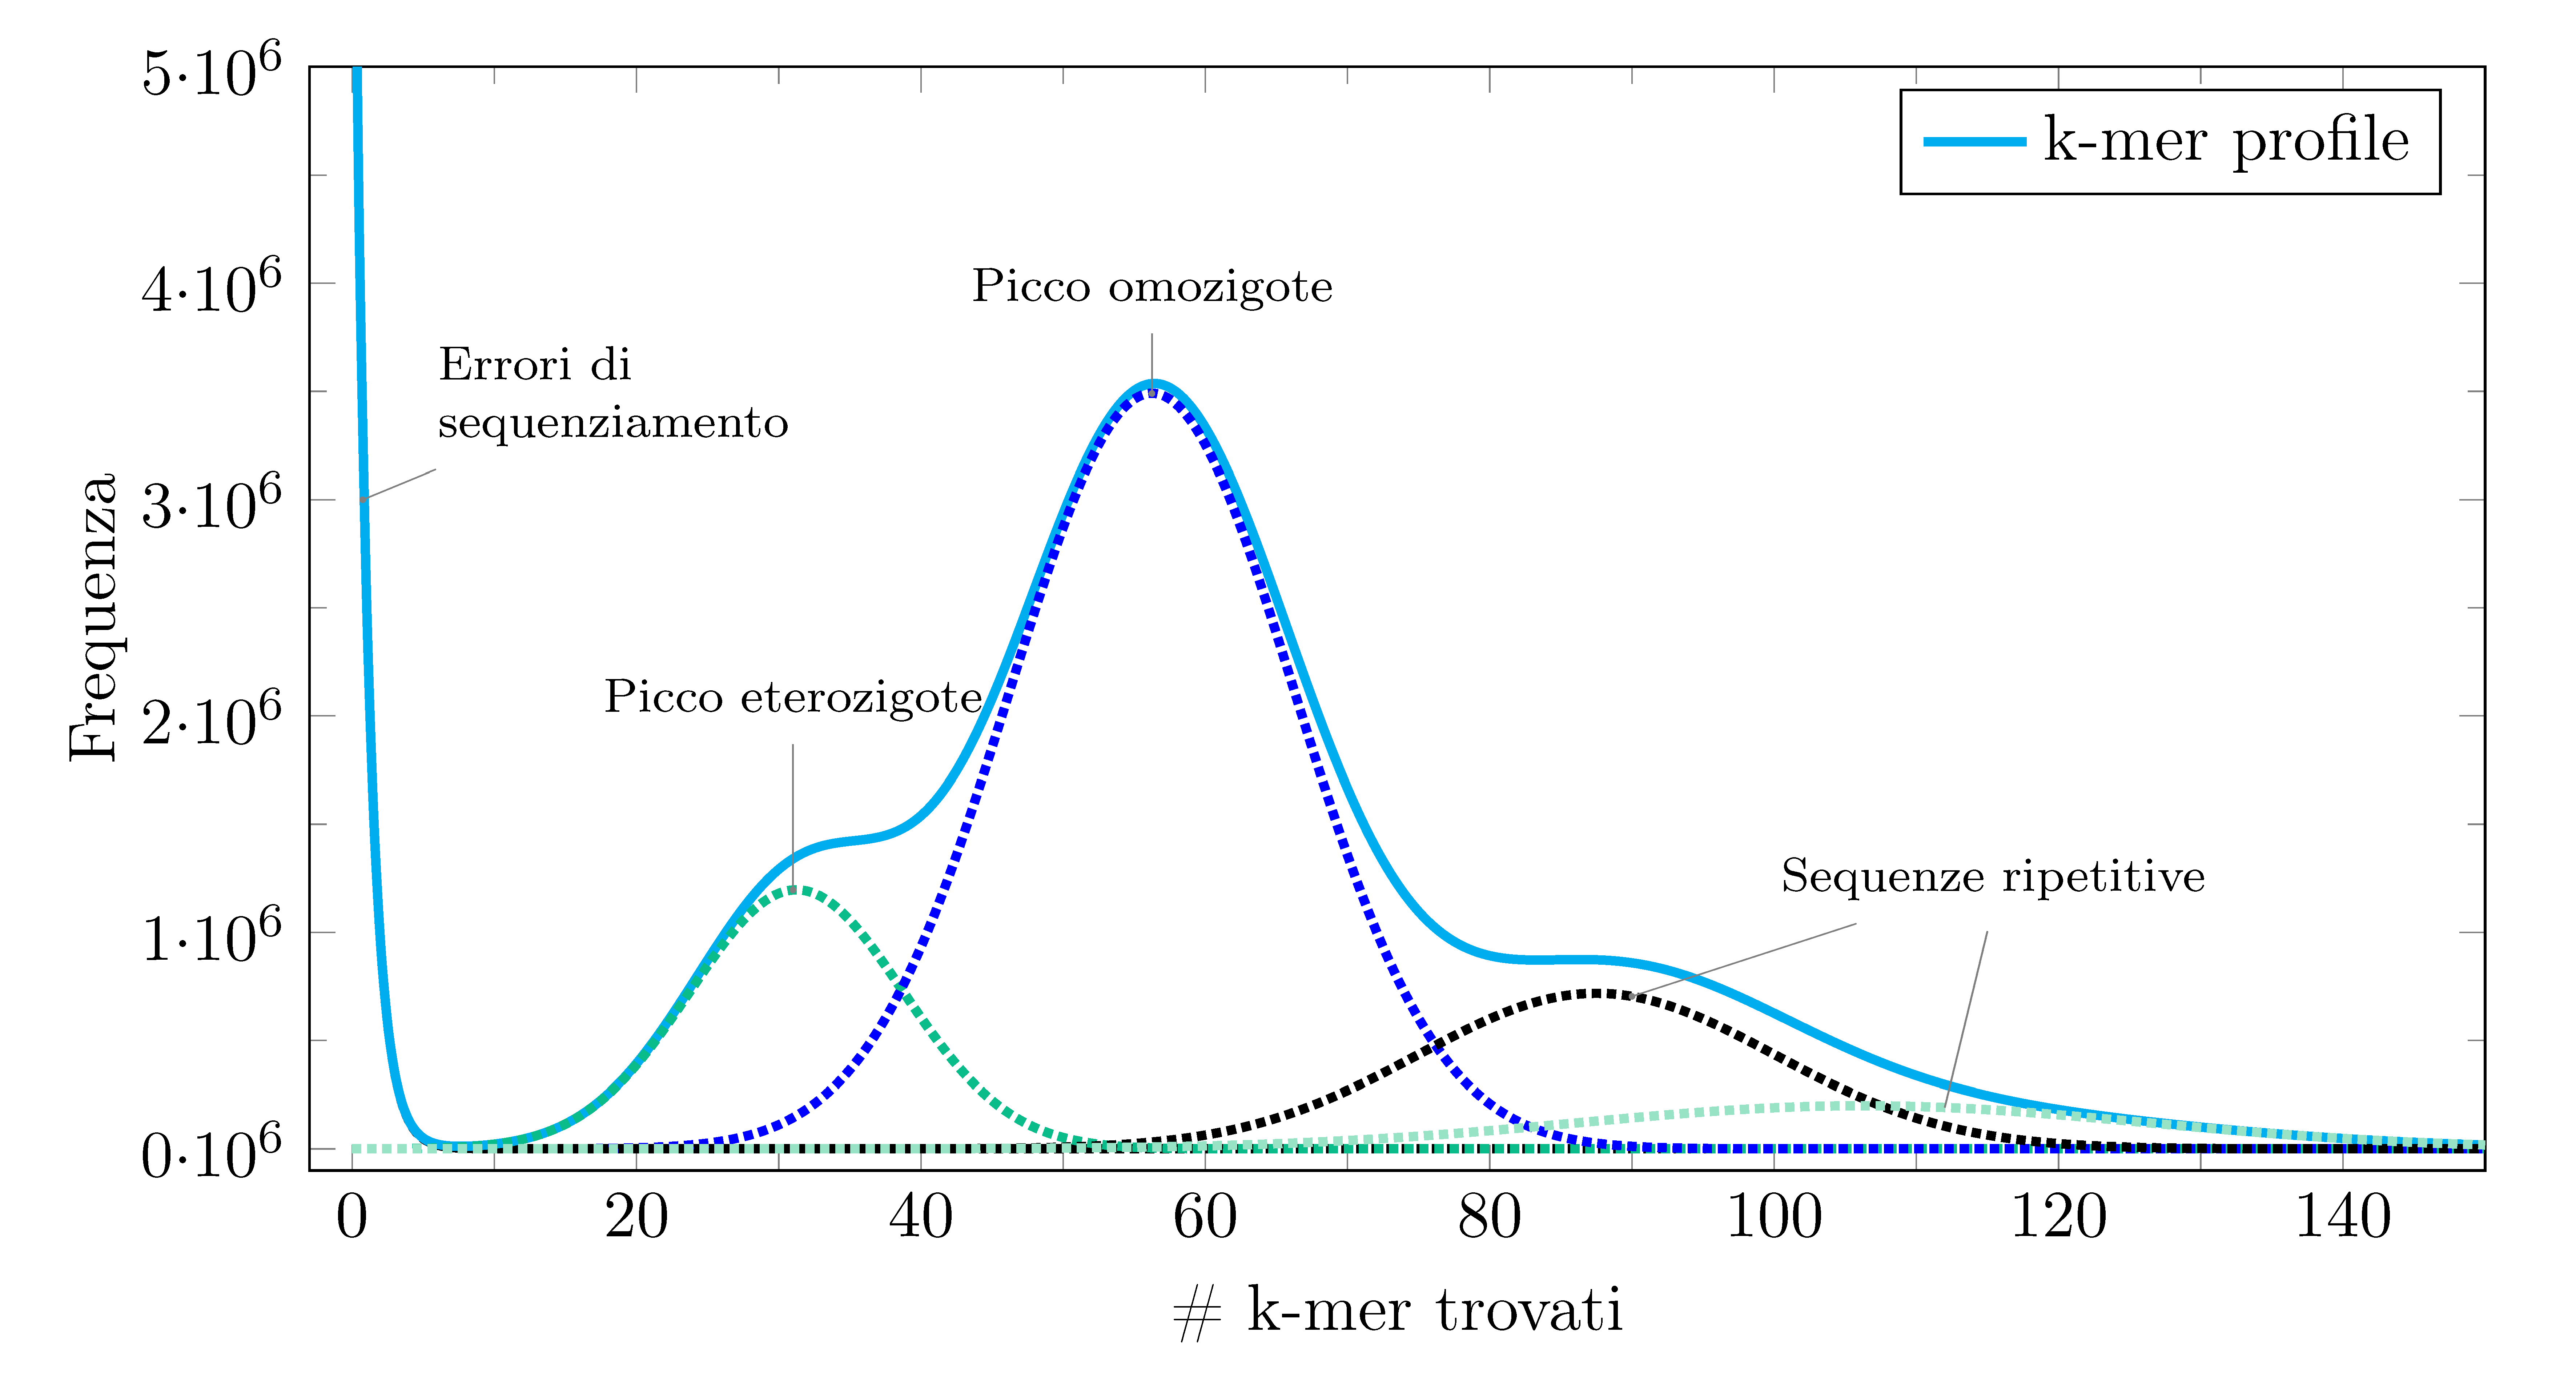
\includegraphics[width=0.8\textwidth]{capitoli/introduzione/profilecomp.png}
		\caption{TODO.}
		\label{fig:profilecomp}
	\end{figure}
	
	Ipotizzando che il genoma sia ideale, omozigote e senza ripetizioni, e che le letture siano state fatte senza errori con una certa copertura, il grafico del k-mer profile sarà una \gls{dp} centrata sulla copertura media disponibile.
	
	In casi reali invece, il genoma sarà eterozigote con una certa percentuale di eterozigosi e saranno presenti errori di sequenziamento; il k-mer profile presenterà tre picchi principali~\cite{sun2017findGSE}.
	Il primo picco del grafico corrisponde ai k-mer derivati da errori di sequenziamento, che accadono spesso ma che hanno bassa frequenza perché presentano poche occorrenze nelle letture di input; il secondo invece, rappresenta i k-mer eterozigoti e il terzo quelli omozigoti, presenti quindi su uno o entrambi gli alleli del set di cromosomi. I k-mer eterozigoti devono essere trattati più attentamente, perché possono risultare simili a quelli del primo picco, derivanti da errori di sequenziamento~\cite{sohn2016present}.	
	
	La lunga coda della distribuzione rappresenta invece le sequenze ripetitive, che occorrono con alta frequenza e sono presenti in un elevato numero di \gls{locus}. Eventuali ripetizioni aggiungono al grafico ulteriori picchi, mentre errori nelle letture aumentano la varianza e producono distorsioni nel grafico.
	
	La figura~\vref{fig:kmerprofile} mostra come all'aumentare del \gls{rate_eterozigosity} la quantità di k-mer eterozigoti del secondo picco diventi dominante rispetto ai k-mer omozigoti del terzo picco, che invece diminuiscono.
	
	Il k-mer profile può essere calcolato tramite programmi specifici date delle letture del genoma di input, quali \textit{Jellyfish}~\cite{marcais2011fast} o \textit{KMC2}~\cite{deorowicz2015KMC}.
	
	
	
	
	\begin{figure}
		\centering
		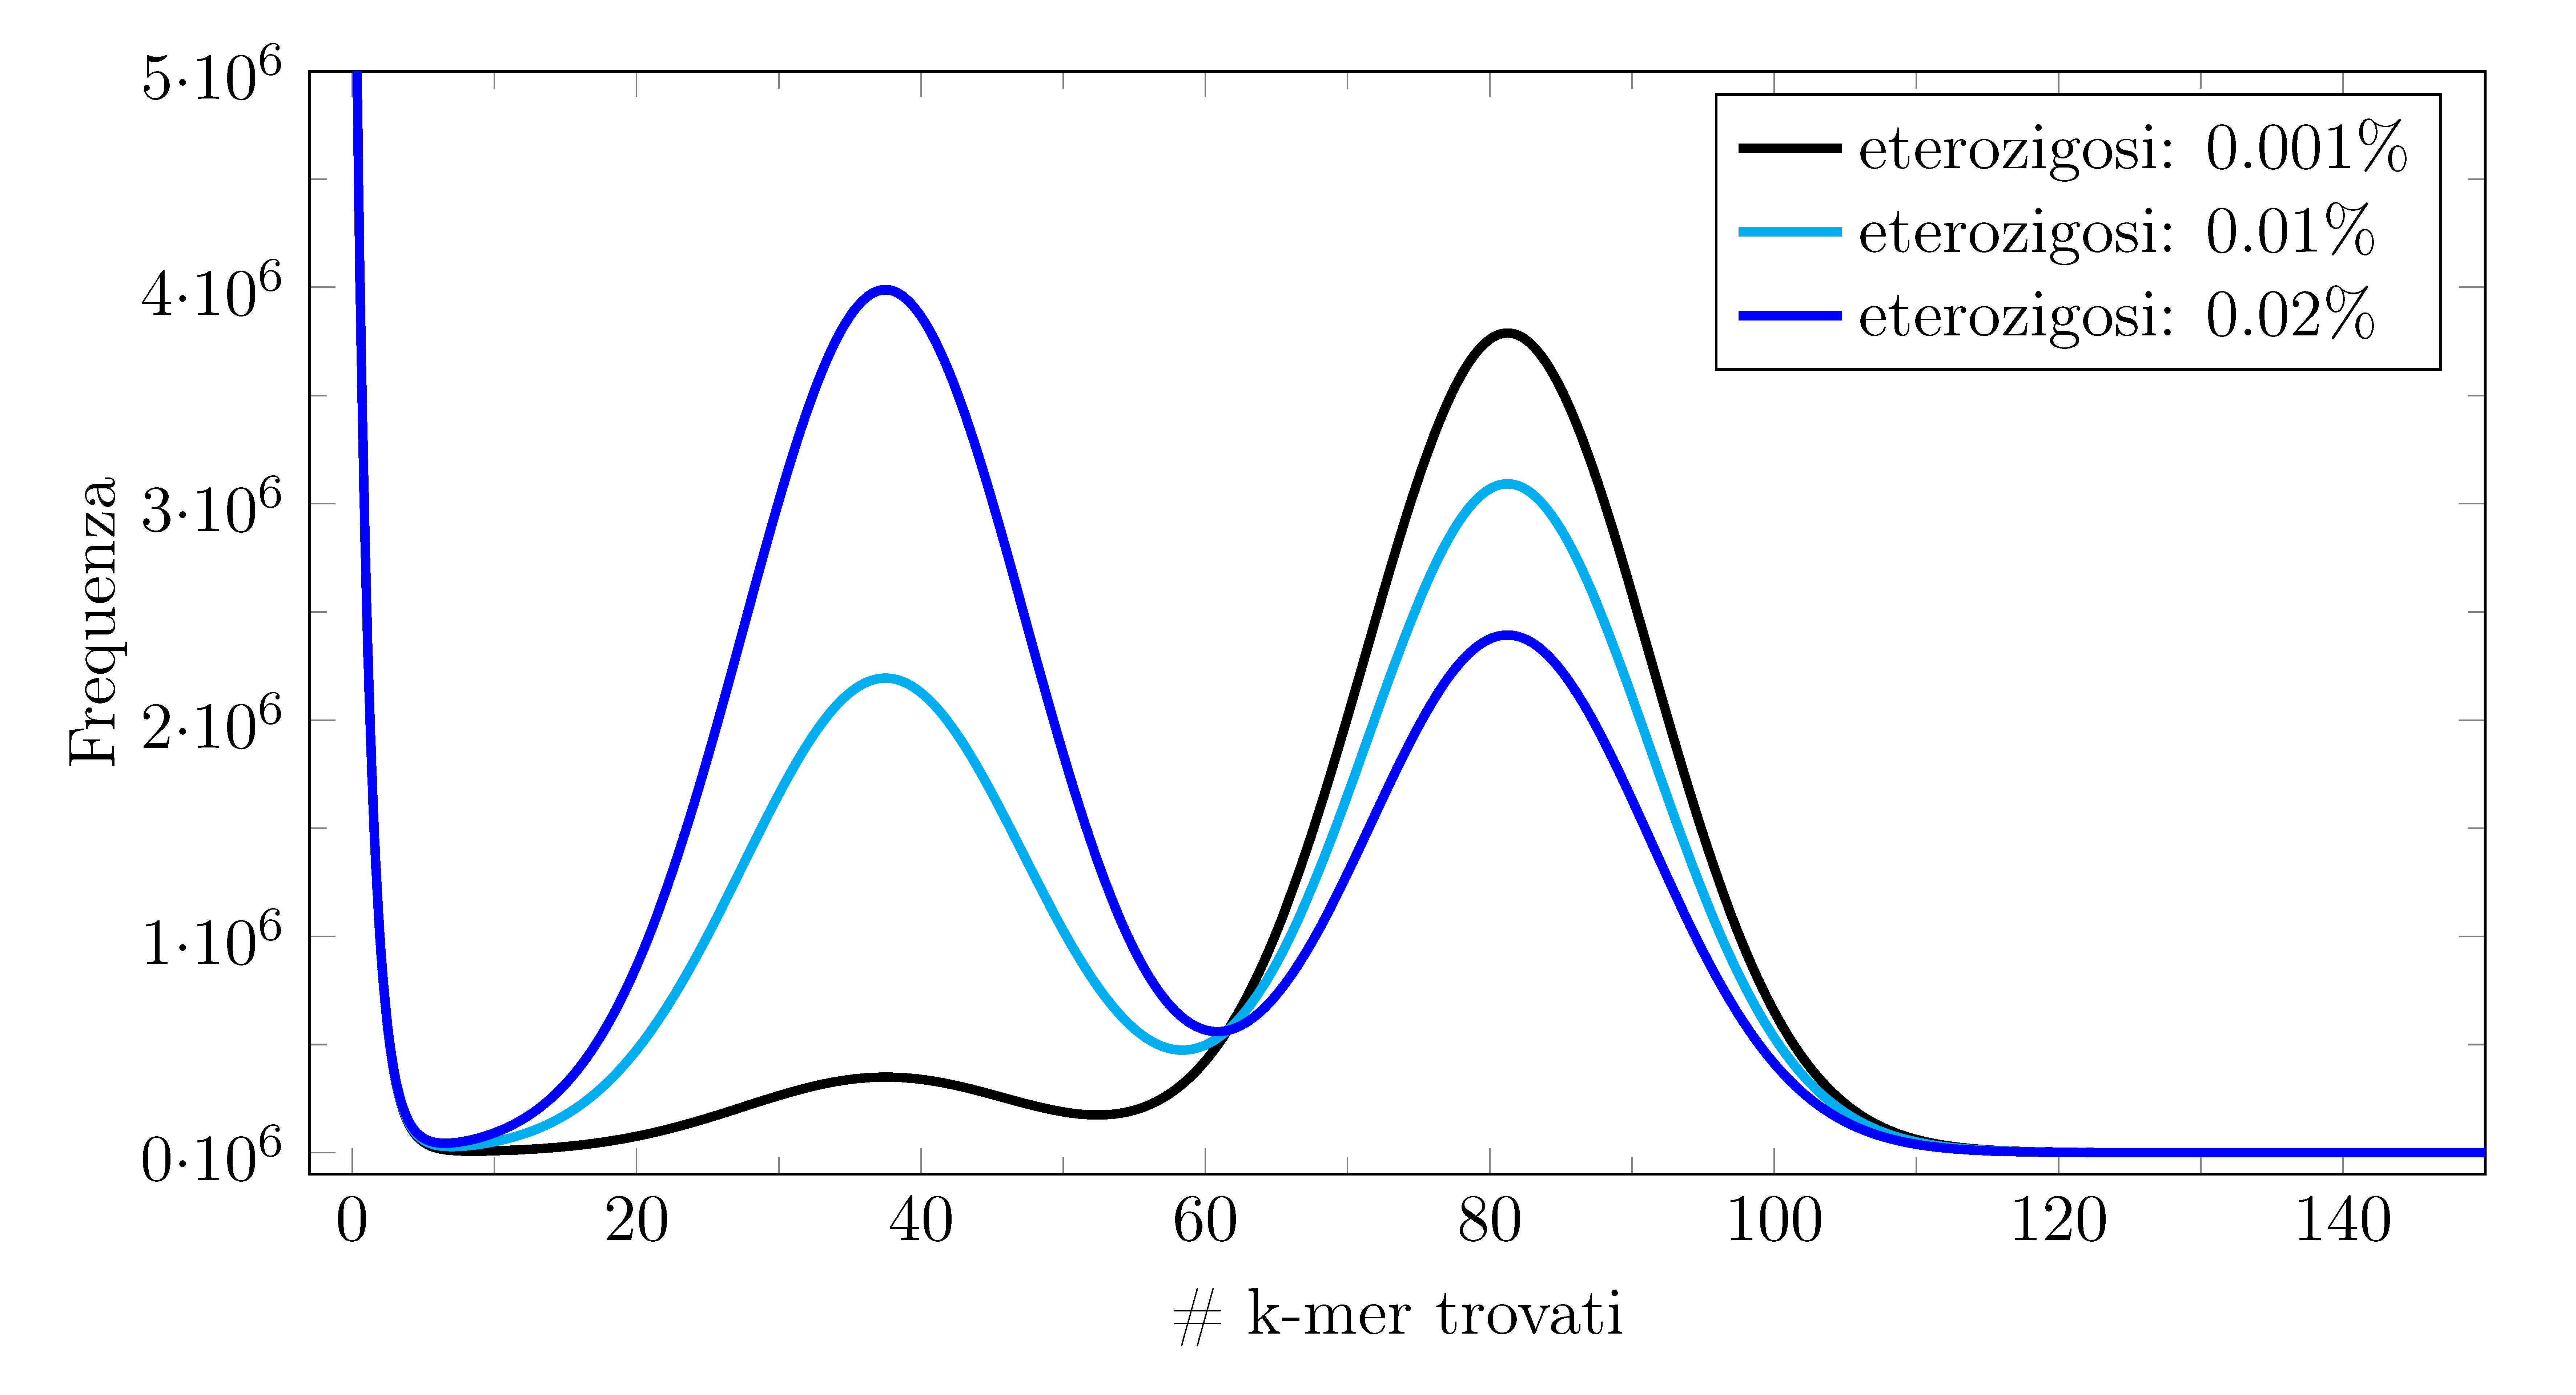
\includegraphics[width=0.8\textwidth]{capitoli/introduzione/kmerprofile.png}
		\caption{TODO.}
		\label{fig:kmerprofile}
	\end{figure}

	%\lipsum[1]
	%\section{Lorem ipsum}
	%\lipsum[2]
	%\subsection{Dolor sit amet} 
	%\lipsum[3]
	%\subsubsection{Lorem ipsum}
	%\lipsum[3]
	
	
	
	
\end{document}
	
	% Capitolo 2
	\documentclass[crop=false, class=book]{standalone}

\begin{document}
	\chapter{Metodi analizzati}
	In questo capitolo vengono presentati, in ordine cronologico di pubblicazione, i metodi presi in esame. Ciascun programma viene descritto svolgendo un'analisi dell'algoritmo che lo caratterizza, ed elencando le funzionalità previste per la gestione di eventi particolari, come ad esempio la presenza di errori di sequenziamento. 
	
\end{document}
	\documentclass[crop=false, class=book]{standalone}

\begin{document}
	
	
	\section{ALLPATHS-LG}
	\label{sec:allpaths}
	\textit{ALLPATHS-LG} è un programma che permette di eseguire il sequenziamento di un genoma tramite de novo assembly di letture shotgun, e che calcola implicitamente la dimensione totale del genoma. Esso si basa sul programma \textit{ALLPATHS}~\cite{butler2008allpaths,maccallum2009allpaths2} sviluppato precedentemente e, rispetto al suo predecessore, permette l'assembly di genomi di dimensioni maggiori e con copertura minore, di gestire sequenze ripetitive, di correggere errori di lettura e di utilizzare in modo più efficiente le risorse disponibili durante il sequenziamento~\cite{gnerre2011high}. 
	
	
	\subsection{Algoritmo}
	L'algoritmo del programma si basa sul precedente software ALLPATHS~\cite{butler2008allpaths}. Dato un numero minimo $k$ di basi che si sovrappongono nelle letture shotgun, si definisce \textit{branch} una sequenza di $k$ basi (k-mer) che compare in due o più letture diverse, e la cui base successiva o precedente è diversa in ogni lettura. Spezzando il genoma in corrispondenza di ciascun branch, esso viene scomposto in un insieme di sequenze, dette \textit{unipath}. Tali sequenze vengono create a partire dalle letture shotgun di input non allineate. 
	
	\paragraph{Formazione dei k-mer path}
	Inizialmente negli shotgun viene corretto il maggior numero di errori di lettura, e vengono poi riconosciuti tutti i k-mer di lunghezza $k$. In ogni sequenza, ciascun k-mer viene numerato con un numero intero unico; a k-mer già trovati viene assegnato lo stesso valore. In questo modo ciascuna lettura potrà essere espressa come una sequenza di numeri interi, ognuno dei quali rappresenta un k-mer. 
	
	I numeri della sequenza vengono poi raggruppati in intervalli, in modo da formare i \textit{k-mer path}; essi associano ciascun intervallo al k-mer path a cui esso appartiene, permettendo una facile ricerca di tutte le sequenze che condividono un certo k-mer e semplificando quindi l'assembly delle letture shotgun. Si veda la figura~\vref{fig:allpathsnumbering} per un esempio di come avviene la numerazione dei k-mer e la creazione dei k-mer path.
	Le letture così tradotte costituiscono il database in cui è possibile effettuare ricerche per la costruzione degli unipath.
	
	\begin{figure}
		\centering
		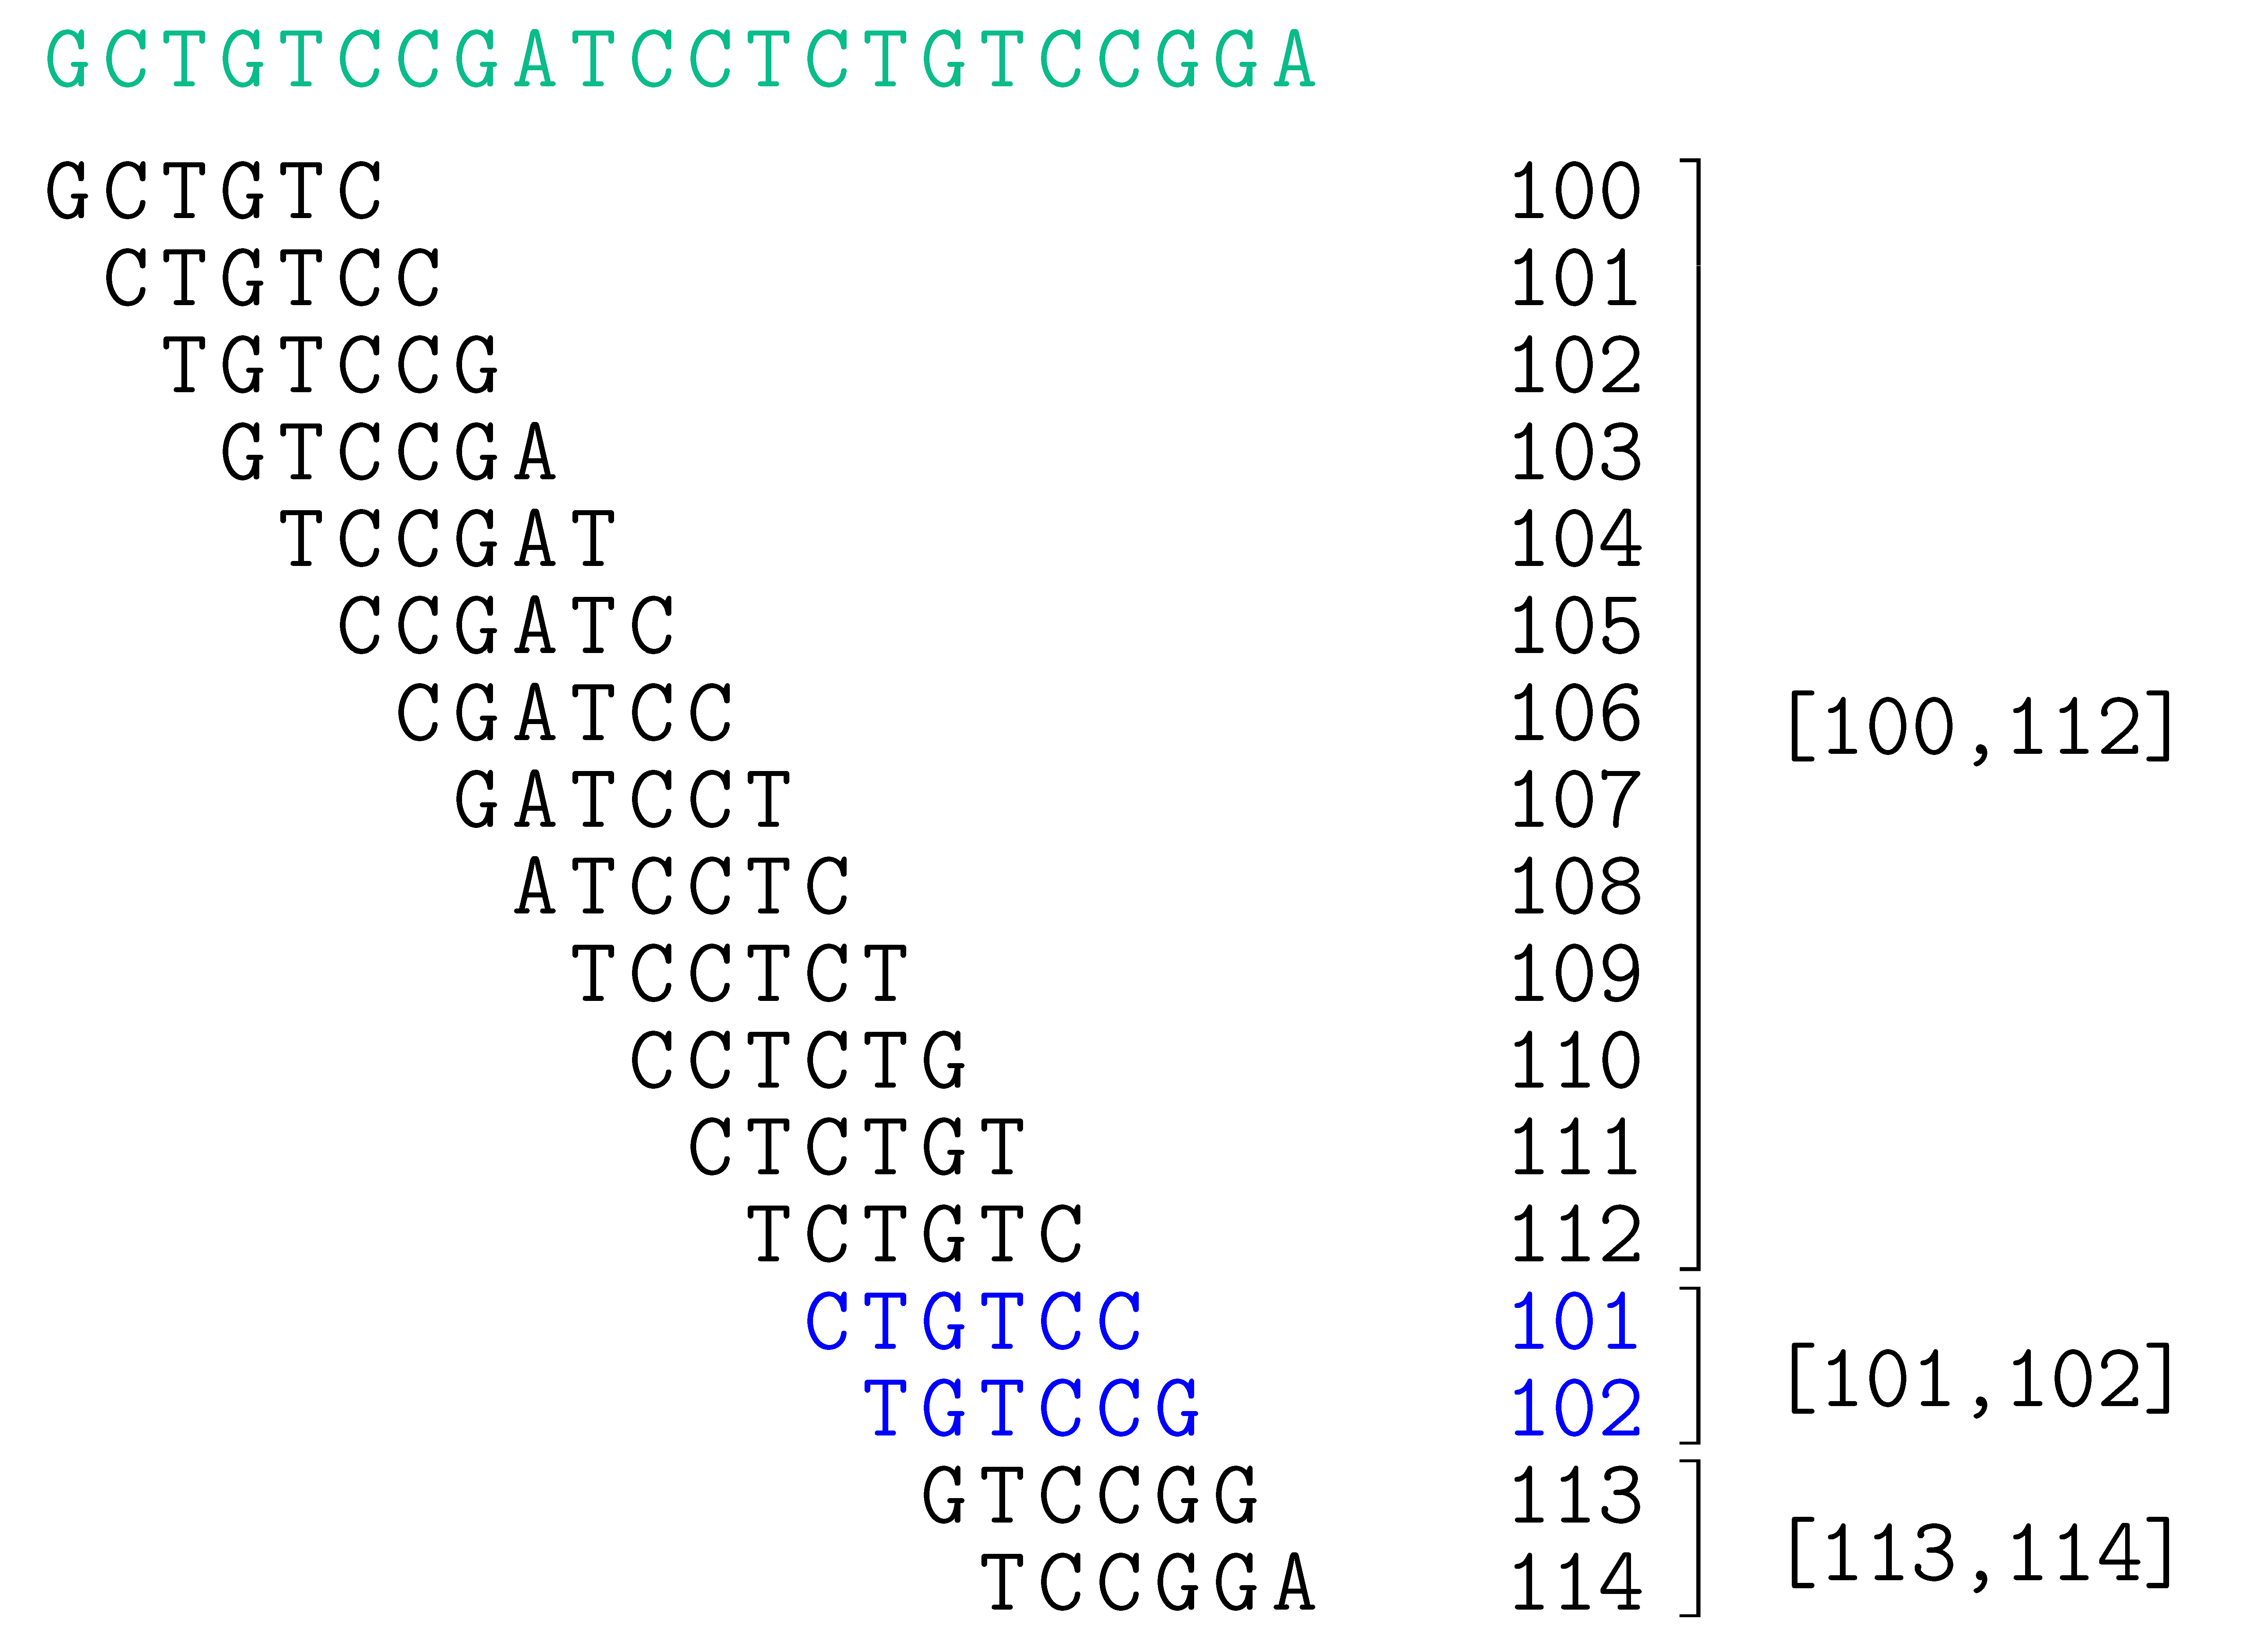
\includegraphics[width=0.6\textwidth]{capitoli/metodi analizzati/allpaths/numbering.png}
		\caption{Esempio di numerazione dei k-mer e traduzione della sequenza in intervalli. Posto $k=6$, vengono individuati tutti i k-mer presenti, ognuno dei quali viene numerato con un numero unico, riutilizzandolo nel caso di k-mer ripetuti. Usando gli intervalli, la sequenza iniziale viene quindi tradotta in $([100,112], [101, 102], [113, 114])$.}
		\label{fig:allpathsnumbering}
	\end{figure}
	
	\paragraph{Formazione degli unipath}
	Tutti i numeri degli intervalli trovati nei k-mer path vengono scanditi. L'obiettivo per ogni numero è trovare il più lungo intervallo senza interruzioni che lo contenga. Si cercano nel database tutti gli intervalli che contengono quel numero, e si sceglie l'intervallo continuo più lungo, che diventa un \textit{unipath interval}. Il processo è ripetuto per tutti i k-mer che non sono stati ancora inclusi in un unipath interval. 
	
	Per ogni unipath interval viene preso il primo numero di k-mer; esso viene cercato nel database e, a partire da quest'ultimo, si determina, se presente, un suo possibile predecessore. Se ne esiste esattamente uno, l'unipath interval del primo numero viene collegato all'intervallo alla sua sinistra. Procedendo iterativamente, viene formato un unipath, che consiste quindi in un gruppo di k-mer contigui. 
	
	\paragraph{Isolamento dei seed unipath}
	Tra gli unipath creati, è possibile isolare dei \textit{seed unipath} attorno ai quali poi eseguire l'assembly. Preso l'insieme di tutti gli unipath, iterativamente si rimuovono alcuni di essi; quindi, preso un certo unipath $u$, si isolano quelli adiacenti a destra e a sinistra rispetto a $u$. Tra i due vicini di $u$ viene dedotta la distanza; se essa è minore di una certa soglia, $u$ può essere rimosso dall'insieme. Si procede in questo modo per tutti gli unipath presenti finché continua a essere possibile la rimozione. Gli unipath rimasti costituiranno un seed unipath.
	
	\paragraph{Assembly locale e globale}
	Attorno ai seed unipath viene quindi assemblato il vicinato (\textit{neighborhood}), cioè le regioni di 10 kb che precedono e seguono il seme. Per farlo, vengono creati due gruppi di sequenze, il primo (\textit{primary read cloud}) contenente letture la cui posizione reale è vicina al seme, mentre il secondo (\textit{secondary read cloud}) contiene brevi frammenti la cui sequenza può essere assemblata con le letture del primo gruppo. Il vicinato dei semi viene quindi assemblato utilizzando i due gruppi di letture, formando un \textit{sequence graph} dell'assembly locale, cioè attorno al seed unipath corrispondente.
	
	I vari assembly locali vengono fatti in parallelo e sono poi uniti per formare un sequence graph unico, relativo cioè all'assembly globale.
	
	
	\subsection{Gestione di genomi di grandi dimensioni}
	I predecessori di ALLPATHS-LG ottengono risultati promettenti solo per genomi di piccole dimensioni. Per gestire genomi di dimensioni più grandi, come quelli dei mammiferi, sono state fatte delle modifiche notevoli~\cite{gnerre2011high}.

	Il programma cerca di comprimere le ripetizioni in modo da favorirne l'allineamento. Se una sequenza ripetitiva è presente in due letture separate, il programma utilizza un'altra coppia di shotgun per poter allineare le prime due (\textit{gap filling}). Le letture vengono unite se un'altra coppia fornisce una sovrapposizione, e viceversa. Il metodo può essere utilizzato anche se sono presenti \glspl{snp}, che forniscono più soluzioni di assemblamento. La figura~\vref{fig:allpathsfilling} tratta da~\cite{gnerre2011high}, mostra come avviene la gestione delle sequenze ripetitive nei due diversi casi.

	\begin{figure}
		\centering
		\subfloat[][\emph{L'allineamento della coppia di letture in nero è possibile usando un'altra coppia di letture, raffigurate in rosso.}]
		{
\includegraphics[width=0.6\textwidth]{capitoli/metodi analizzati/allpaths/filling1.png}} \\
		\subfloat[][\emph{Le due coppie di letture in rosso potrebbero allineare la coppia di letture in nero, ma presentano una mutazione \gls{snp}. Vengono quindi mantenute entrambe, fornendo due diverse soluzioni possibili.}]
		{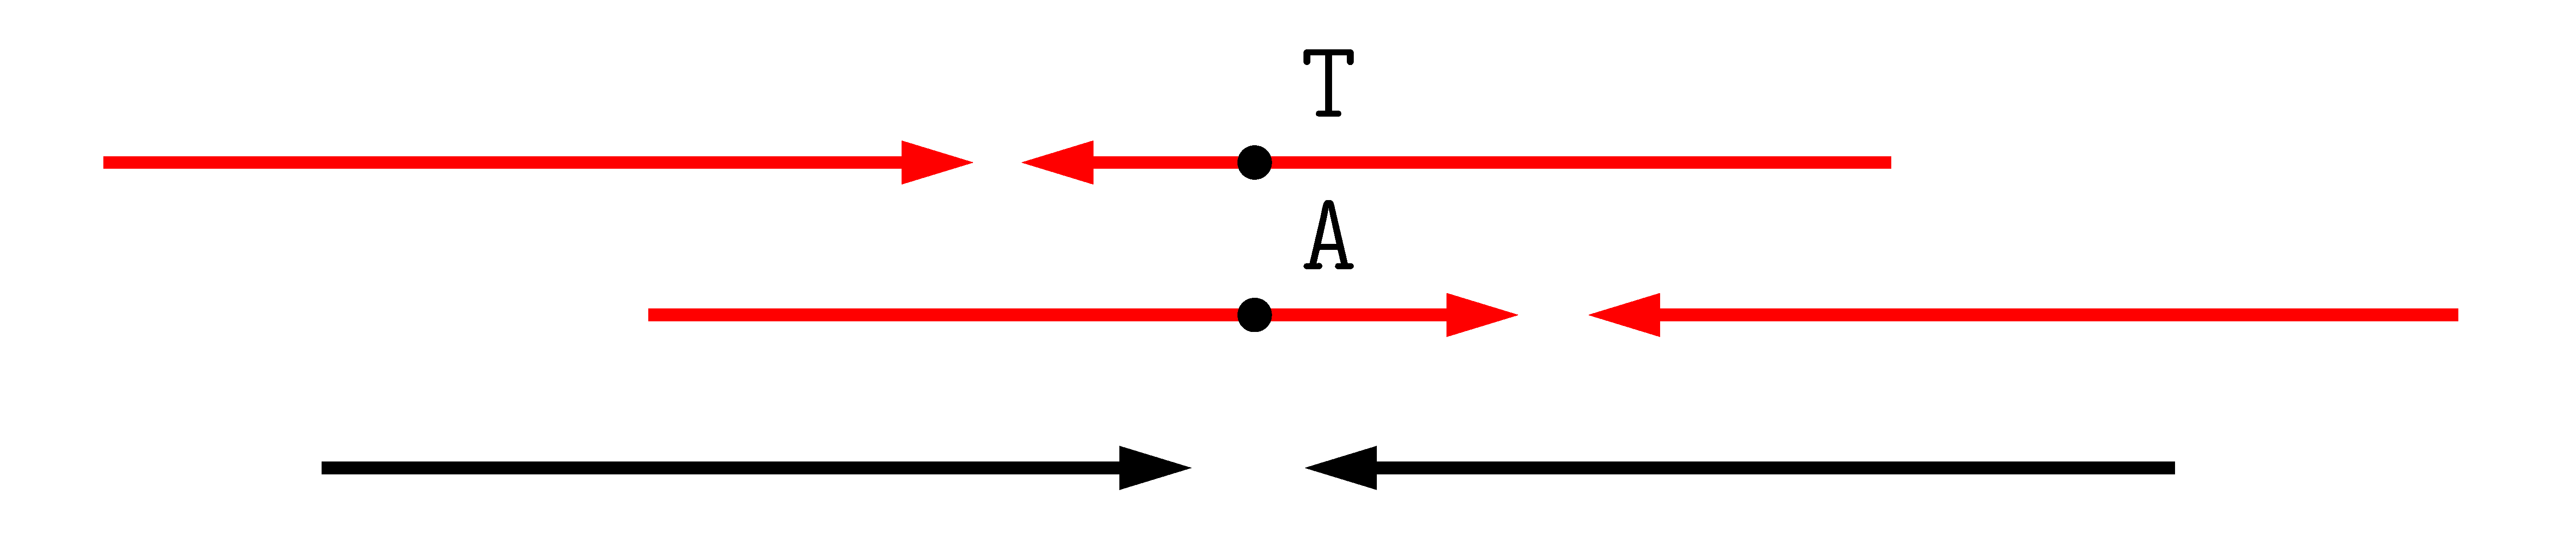
\includegraphics[width=0.6\textwidth]{capitoli/metodi analizzati/allpaths/filling2.png}} 
		\caption{Esempi grafici del processo di gap filling.}
		\label{fig:allpathsfilling}
	\end{figure}
	
	La nuova versione del programma, inoltre, migliora la correzione degli errori di lettura: dato un k-mer, vengono analizzate tutte le letture che lo contengono; nel caso in cui una singola lettura differisca dalla maggior parte delle altre, essa viene corretta se non ci sono voti in conflitto, altrimenti non viene modificata.
	
	Ulteriori miglioramenti sono stati applicati anche per la gestione di sequenze a bassa copertura: dato che in questi casi la sovrapposizione tra letture può essere breve, in tali zone è preferibile utilizzare k-mer di dimensioni minori cioè scegliere un valore di $k$ più basso. Il programma permette di utilizzare un valore di $k>15$, ma solo nelle regioni che verrebbero assegnate a uno spazio vuoto tra altre due sequenze. 
	
	\subsection{Stima della dimensione del genoma}
	Il programma, pur avendo come scopo primario la costruzione dell'assembly a partire dalle letture del genoma, produce in output un valore stimato della sua dimensione. Per farlo, dato il grafico del k-mer profile, esso identifica l'ascissa del punto di flesso $f_v$ che si trova tra il primo e il secondo picco, cioè tra quello dei k-mer derivanti da errori di sequenziamento e quello dei k-mer omozigoti, e l'ascissa $f_p$ corrispondente al picco eterozigote \cite{sun2017findGSE}.
	
	La dimensione del genoma $G$ viene quindi stimata considerando gli $N$ k-mer con copertura $C$ compresi tra $f_v$ e $3f_p/2$, scartando quindi dalle letture i k-mer a frequenze basse o molto alte, tramite la formula $G = N/C$.

\end{document}
	\documentclass[crop=false, class=book]{standalone}

\begin{document}
	\section{GCE}
	\label{sec:GCE}
	Il programma \textit{GCE} permette di modellare la distribuzione dei k-mer presenti nei dati sequenziati e di stimare la dimensione del genoma, le sequenze ripetitive e il rapporto di eterozigosi~\cite{liu2013GCE}. Il programma è open-source, scritto in C/C++ e si basa sulla statistica bayesiana.
	
	\subsection{Algoritmo}
	\paragraph{Conteggio dei k-mer}
	Il programma fa uso del k-mer profile delle letture disponibili per stimare le caratteristiche del genoma. Inizialmente deve essere determinato il valore ottimale di $k$, che deve risultare grande abbastanza da far apparire ogni k-mer quasi unico all'interno del genoma, ma allo stesso tempo il più piccolo possibile per evitare un uso eccessivo di memoria durante l'estrazione dei k-mer. Per questo di solito si preferisce un valore $k$ tale che $4^k>5 \times G$, con $G$ dimensione del genoma. In base al valore $k$ scelto, può essere calcolato il k-mer profile.
	Il programma utilizza, oltre alle letture del genoma da sequenziare, un genoma di riferimento (\textit{reference genome}).
	
	\paragraph{Modello ideale}
	Inizialmente, ipotizzando che entrambi i genomi siano ideali, cioè che il reference genome sia una sequenza casuale, senza eterozigosi o ripetizioni, e che le letture del genoma da sequenziare siano di uguale lunghezza e senza errori di sequenziamento, la distribuzione delle frequenze dei k-mer seguirà una distribuzione di Poisson~\cite{li2003estimating}. Considerando i valori $n_{base}$ e $n_{k-mer}$ il numero totale di basi e k-mer presenti nelle letture, e rispettivamente $c_{base} = n_{base}/G$ e $c_{k-mer} = n_{k-mer}/G$ le coperture per le basi e i k-mer nelle letture da sequenziare, una lettura di $L$ basi genera $L-k+1$ k-mer, quindi $n_{k-mer} / n_{base} = (L-k+1)/L$. Si ricavano di conseguenza l'equazione~\vref{eqn:GCE1} per il calcolo della copertura delle basi, e l'equazione~\vref{eqn:GCE2} per la lunghezza del genoma.
	
	\begin{equation}
		\label{eqn:GCE1}
		c_{base} = c_{k-mer} \times L / (L-k+1);
	\end{equation}

	\begin{equation}
		\label{eqn:GCE2}
		G = n_{k-mer} / c_{k-mer} = n_{base} / c_{base}.
	\end{equation}
	
	Utilizzando i simboli $n = n_{k-mer}$ e $c = c_{k-mer}$, l'algoritmo deve determinare entrambi i parametri, per poi calcolare la lunghezza del genoma tramite l'equazione~\vref{eqn:GCE2}.
	
	Il valore $n$ può essere dedotto facilmente dal k-mer profile, ricavato il precedenza, come numero totale dei k-mer trovati. Per il valore della copertura $c$ invece, vengono utilizzate le formule delle distribuzioni di Poisson~\vref{eqn:GCE3}~e~\vref{eqn:GCE4}, che descrivono rispettivamente il k-mer profile, il quale rappresenta il numero di specie di k-mer ($P_{Kspecies}$), e il prodotto tra i valori del numero di specie di k-mer e la copertura, che rappresenta il numero di individui di k-mer ($P_{Kindividuals}$); $x$ si riferisce alla copertura del k-mer profile.
	\begin{equation}
		\label{eqn:GCE3}
		P_{Kspecies}(x) = \frac{c^x}{x!} e^{-c};
	\end{equation}

	\begin{equation}
		\label{eqn:GCE4}
		P_{Kindividuals}(x) = x P_{Kspecies}(x) / c = P_{Kspecies}(x-1).
	\end{equation}
	
	Dalle curve delle distribuzioni, è possibile stimare il valore di $c$ tramite una delle due equazioni~\vref{eqn:GCE5}~o~\vref{eqn:GCE6}.
	\begin{equation}
		\label{eqn:GCE5}
		c = \frac{P_{Kspecies}(x+1)}{P_{Kspecies}(x)} (x+1);
	\end{equation}
	
	\begin{equation}
		\label{eqn:GCE6}
		c = \frac{P_{Kindividuals}(x+1)}{P_{Kindividuals}(x)} x.
	\end{equation}

	\paragraph{Gestione di sequenze ripetitive}
	Nella maggior parte dei casi un genoma reale contiene sequenze ripetitive, le quali aumentano la difficoltà del sequenziamento. Viene quindi utilizzato come riferimento un genoma già sequenziato, nel quale i k-mer vengono classificati in base alla frequenza genomica $i$ (\textit{genomic frequency}), che rappresenta la frequenza dei k-mer nel genoma di riferimento. Per ciascuna classe $i$ vengono calcolati il rapporto delle specie di k-mer ($a_i = n_{i, genomic, Kspecies} / n_{genomic, Kspecies}$) e il rapporto di k-mer individuali ($b_i = n_{i, genomic, Kindividuals} / n_{genomic, Kindividuals}$). 
	Le ripetizioni causano più picchi nel k-mer profile, che possono essere rappresentati come composizione di distribuzioni di Poisson. Le formule delle curve diventano quindi somma di distribuzioni di Poisson, descritte dalle formule~\vref{eqn:GCE7}~e~\vref{eqn:GCE8}.
	\begin{equation}
		\label{eqn:GCE7}
		P_{Kspecies}(x) = \sum_{i=1}^{m} a_i \times P_{Kspecies, i}(x);
	\end{equation}
	
	\begin{equation}
		\label{eqn:GCE8}
		P_{Kindividuals}(x) = \sum_{i=1}^{m} b_i \times P_{Kindividuals, i}(x).
	\end{equation}
	
	La stima del parametro $a_i$ viene fatta iterativamente basandosi su un modello bayesiano, utilizzando la formula~\vref{eqn:GCE9} in cui il termine $v_j$ rappresenta la probabilità della specie di k-mer con copertura $j$, mentre l'espressione $P(j|i)$ rappresenta la probabilità che una specie di k-mer con frequenza $i$ sia trovata $j$ volte nelle letture da sequenziare. Per il parametro $c$ invece è stata ricavata la formula~\vref{eqn:GCE10}, che permette di stimare la dimensione del genoma tramite la formula $G = n_{k-mer}/c$, in cui il termine $ n_{k-mer}$ rappresenta il numero totale di k-mer.
	
	\begin{equation}
		\label{eqn:GCE9}
		a_{i,t+1} = \sum_{j=0}^{w} \frac{a_{i,t} P(j|i)}{\sum_{i=1}^{m} a_{i,t} P(j|i)} \times v_j;
	\end{equation}

	\begin{equation}
		\label{eqn:GCE10}
		c_{t+1} = \frac{P_{Kspecies, 1, t+1}(x+1)}{P_{Kspecies, 1, t+1}(x)} \times (x+1).
	\end{equation}
	
	\paragraph{Sequenziamento di genomi eterozigoti}
	Sequenziando genomi diploidi reali, risulta utile stimare il rapporto di eterozigosi, dovuto a mutazioni \gls{snp}. Posto che i k-mer eterozigoti si distribuiscano in modo sparso nel genoma, saranno presenti $2\times k$ k-mer eterozigoti attorno a ciascun sito SNP, che daranno origine a un nuovo picco nella curva di distribuzione dei k-mer. 
	
	\subsection{Errori di sequenziamento e coverage bias}
	La gestione degli errori di sequenziamento viene fatta considerando i valori stimati di $c$ e $a_i$. Il grafico della distribuzione dei k-mer in questi casi, infatti, presenta un grande picco iniziale, che riduce la dimensione degli altri picchi e li sposta verso sinistra, come mostrato dalla figura~\vref{fig:GCEerrors} tratta da~\cite{liu2013GCE}. Tramite i suddetti valori che rappresentano rispettivamente la copertura e il rapporto delle specie di k-mer, è possibile ricostruire la curva della distribuzione e confrontarla con la curva reale, in modo da determinare il numero di k-mer corretti e rimuovere gli errori di sequenziamento.
	
	\begin{figure}[]
		\centering
		\subfloat[][\emph{Grafici delle specie di k-mer, al variare della percentuale di errore.}]
		{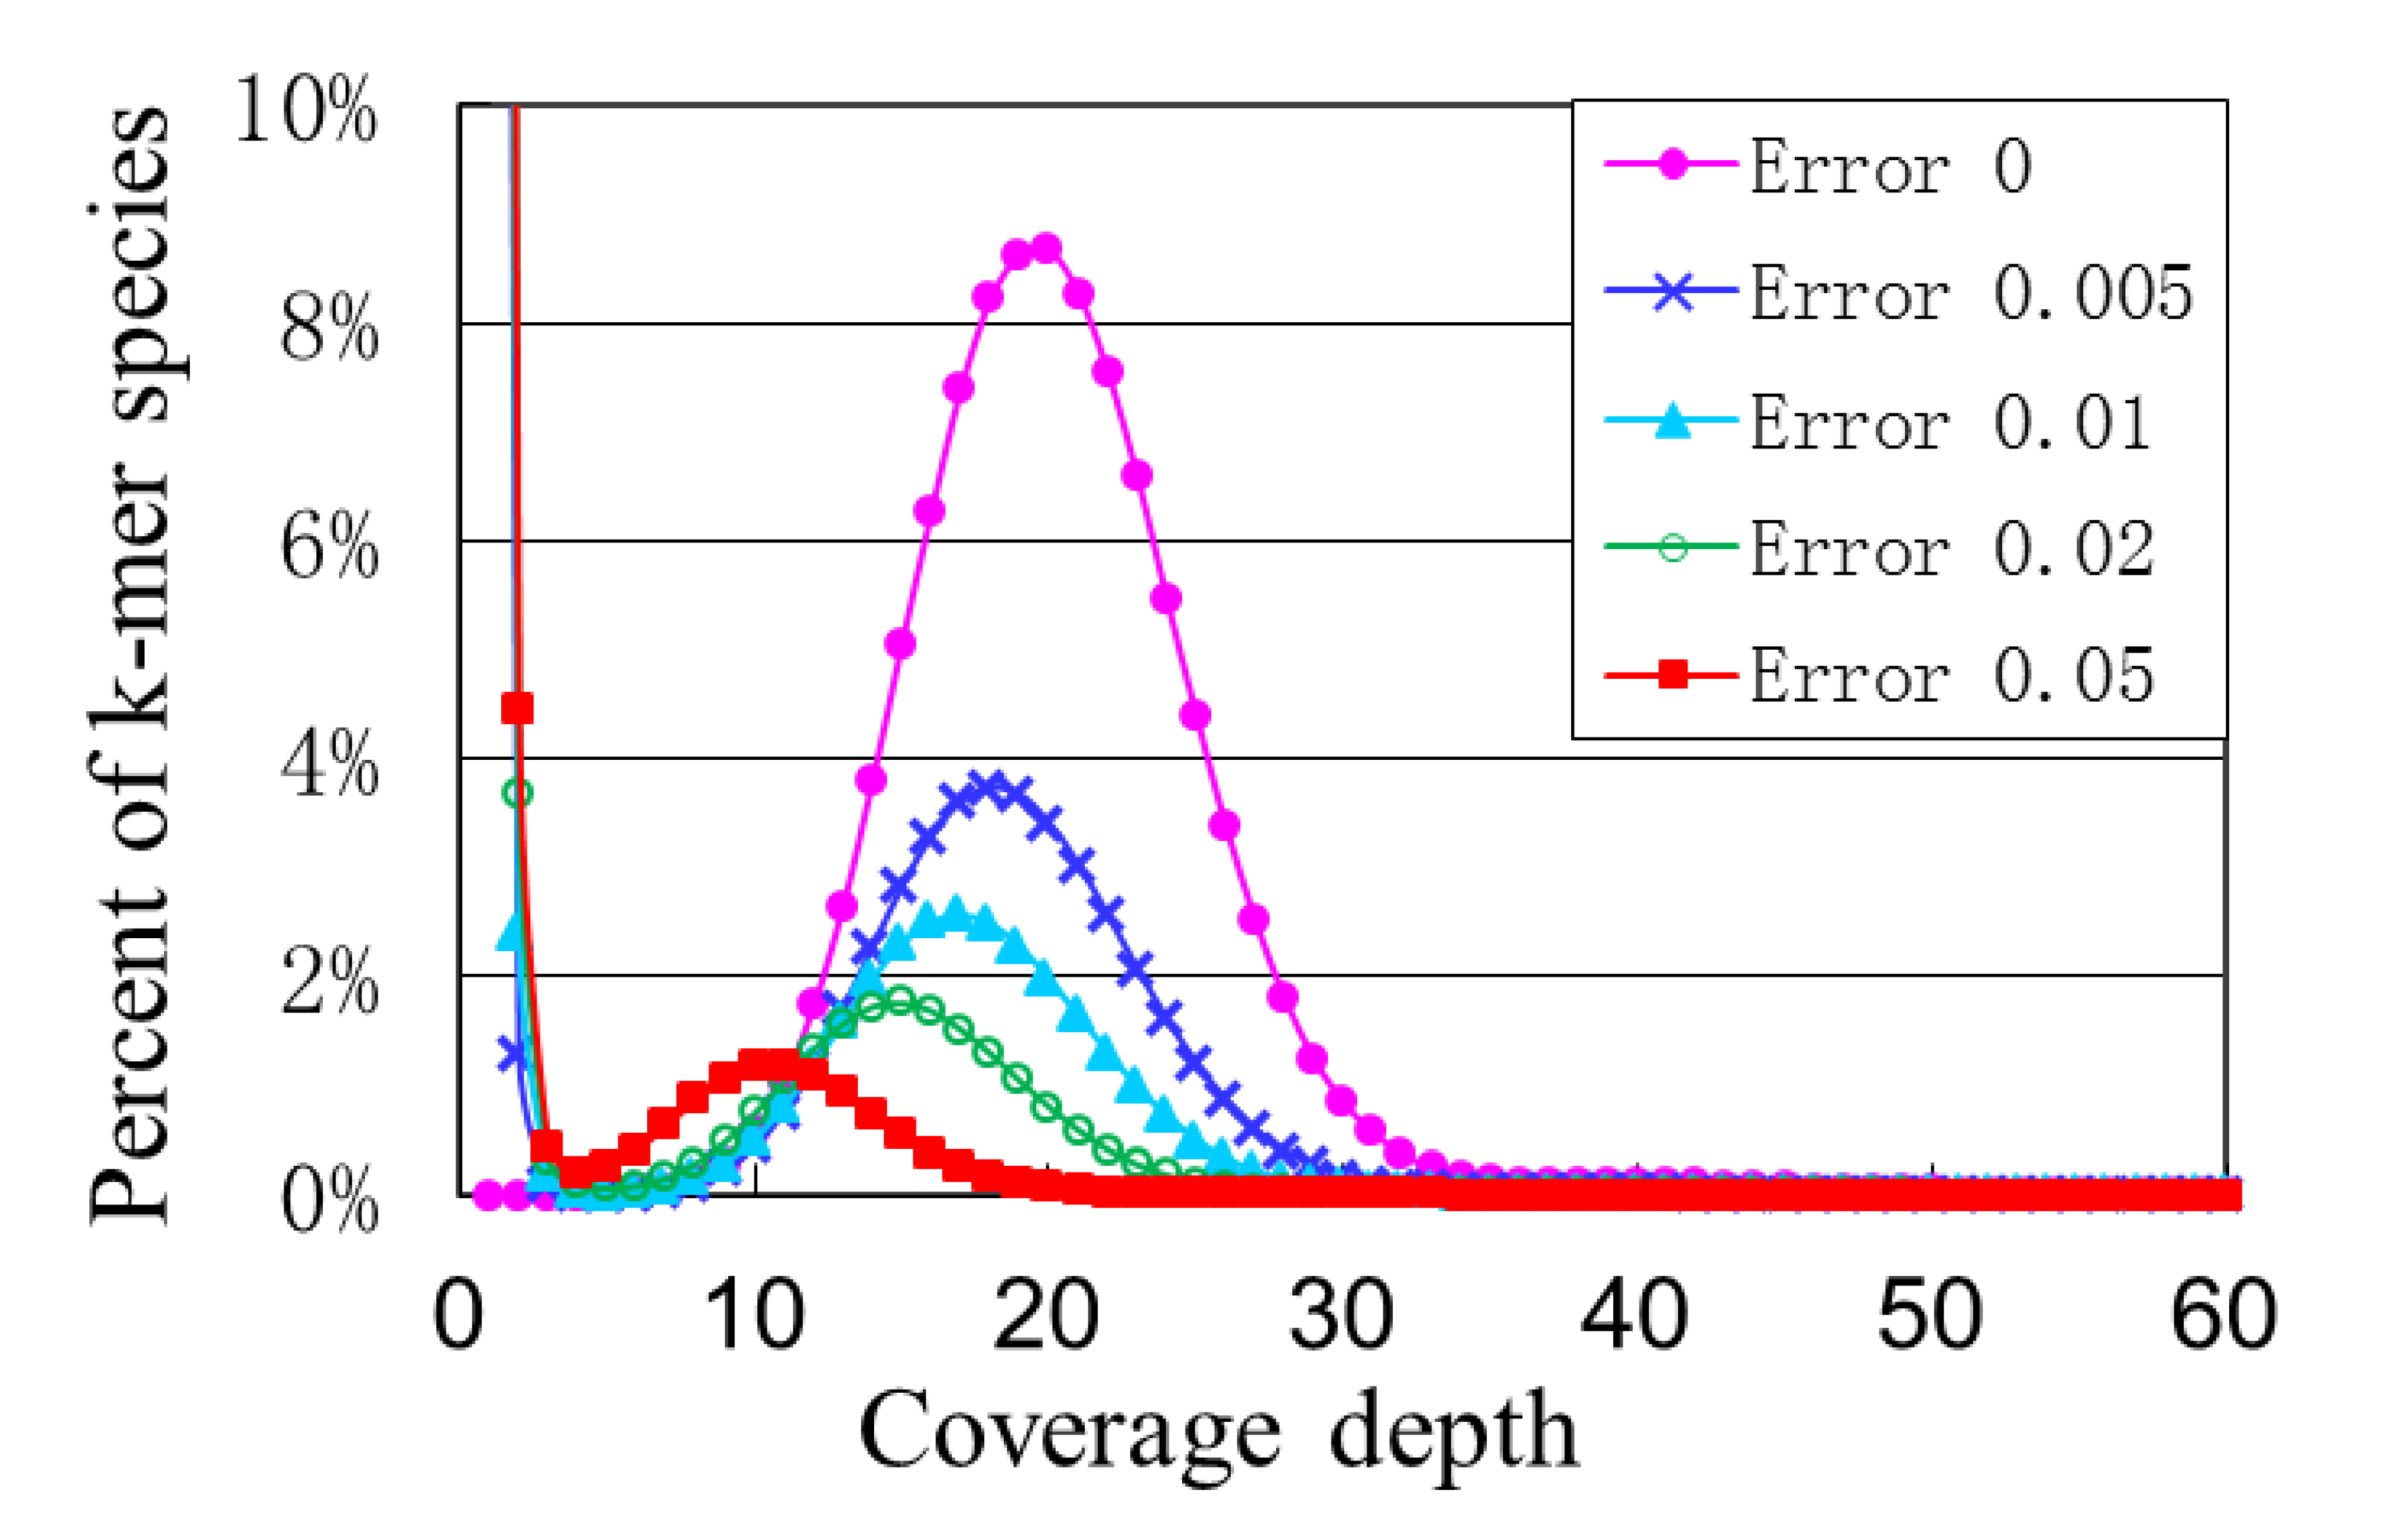
\includegraphics[width=0.48\textwidth]{capitoli/metodi analizzati/GCE/b.png}} \quad
		\subfloat[][\emph{Grafici degli individui di k-mer, al variare della percentuale di errore.}]
		{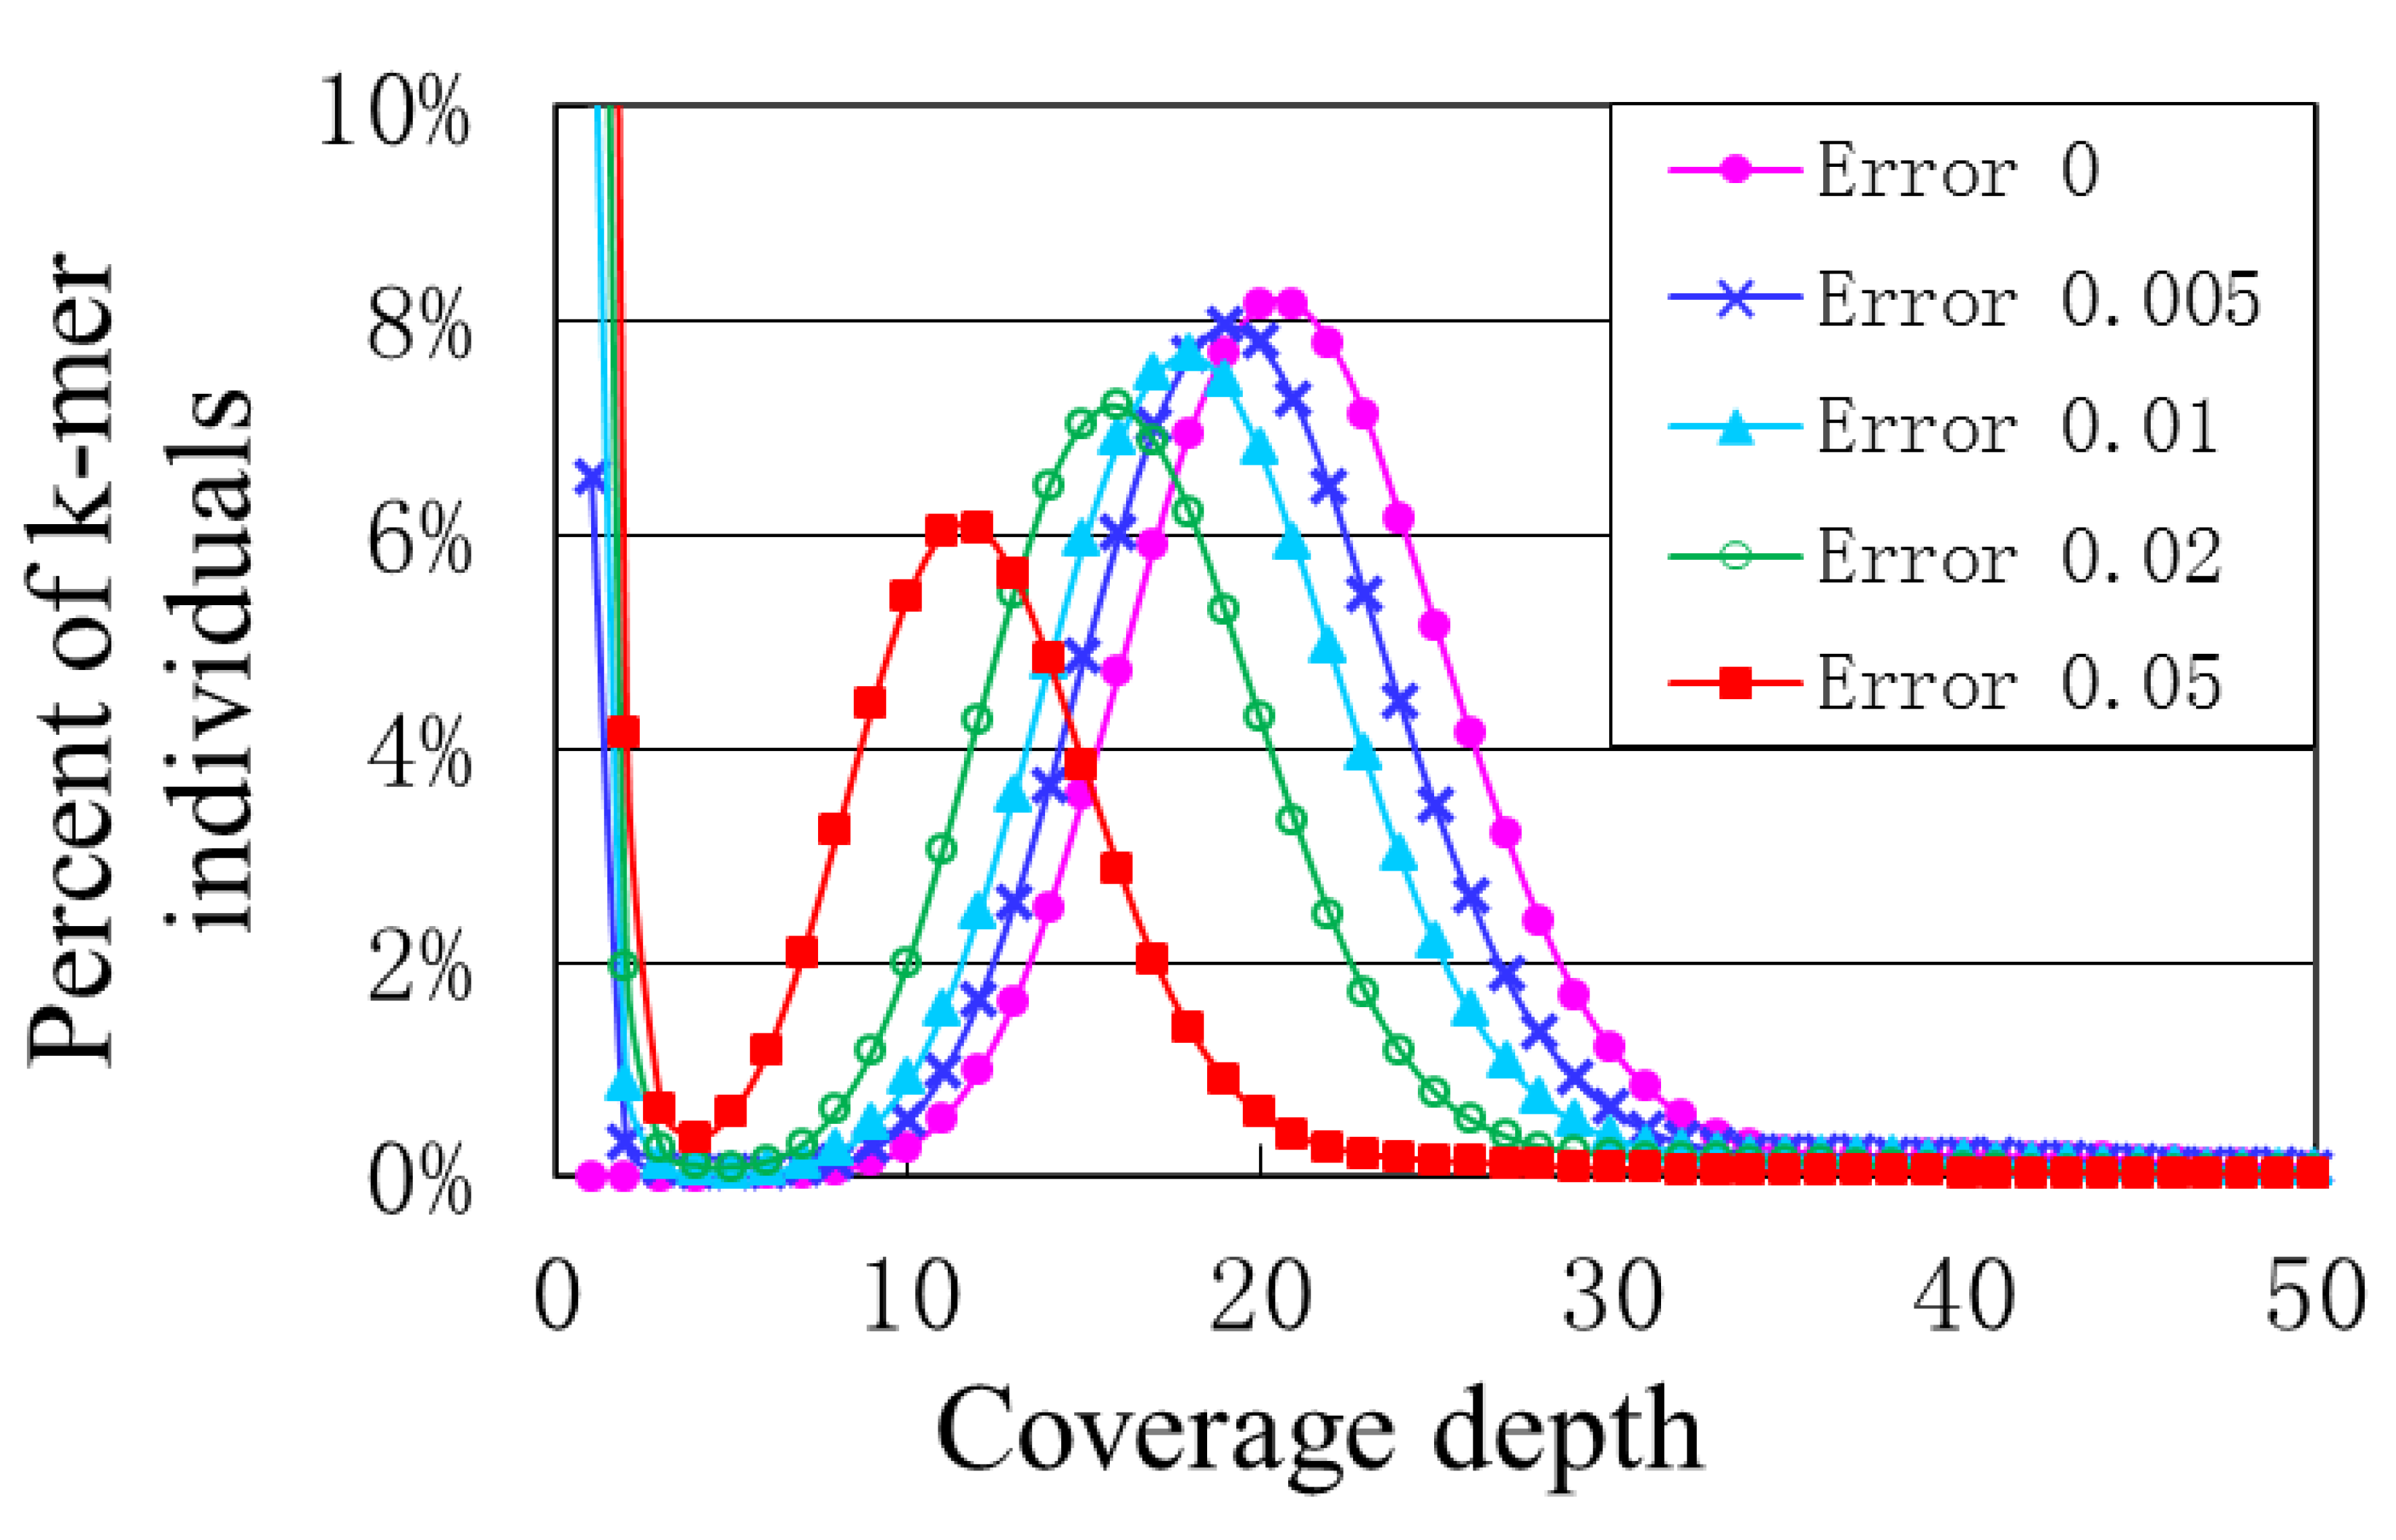
\includegraphics[width=0.48\textwidth]{capitoli/metodi analizzati/GCE/c.png}} 
		\caption{Effetto degli errori di sequenziamento sui grafici delle specie e degli individui di k-mer. Il picco dei k-mer omozigoti viene appiattito e spostato a sinistra all'aumentare della percentuale di errore.}
		\label{fig:GCEerrors}
	\end{figure}
	
	I \textit{coverage bias}, che corrispondono a deviazioni rispetto alla distribuzione uniforme delle letture~\cite{ross2013characterizing}, sono invece più difficili da gestire, poiché appiattiscono le curve rendendo più difficile l'individuazione dei picchi e la stima di $c$. Anche se in presenza di tali errori i k-mer non vengono campionati in maniera equiprobabile, lo spettro di campionamento risulta continuo. Il nuovo modo di rappresentare le distribuzioni di specie e di individui di k-mer diventa quindi un modello continuo, che viene approssimato con un modello discreto a livelli non uniformi $a_k$, nel quale la copertura $c$ scelta corrisponde al maggior valore $a_k$, mentre il parametro $a_i$ viene stimato come somma dei parametri $a_k$ corrispondenti a ciascun picco. Una volta trovati i valori $c$ e $a_i$, viene stimata la dimensione del genoma tramite la formula~\vref{eqn:GCE2}. 
	
\end{document}
	\documentclass[crop=false, class=book]{standalone}

\begin{document}
	\section{GenomeScope}
	\label{sec:GenomeScope}
	Il progetto open source \textit{GenomeScope} cerca sia di stimare le caratteristiche del genoma completo, come ad esempio la sua lunghezza o il rapporto di eterozigosi, sia di determinare le proprietà delle letture di DNA che prende in input, come la copertura (\textit{read coverage}) o l'error rate~\cite{vurture2017genomescope}. Il programma per determinare tali caratteristiche utilizza il k-mer profile del genoma preso in esame, descritto nella sezione~\vref{subsec:kmerprofile}.
		
	\subsection{Algoritmo}
	Il programma effettua una regressione non lineare dei dati iniziali, generando un profilo che cerca di approssimare il k-mer profile reale. Prendendo in input le letture del genoma che si vuole studiare, esso crea un modello che approssima il più possibile il k-mer profile. La funzione $f(X)$ scelta per l'interpolazione delle frequenze dei k-mer trovati è la somma di quattro \glspl{dbn} $Y \sim \mathcal{NB}(X;p,n)$, per rappresentare rispettivamente i k-mer eterozigoti trovati nel genoma diploide una volta (unici) o tre volte (duplicati), e i k-mer omozigoti di cui si trovano due occorrenze (unici) o trovati quattro volte (duplicati). La funzione $f(X)$ è descritta dall'equazione~\vref{eqn:gnmscp_regression}, in cui $G$ rappresenta un coefficiente di scala legato alla dimensione del genoma, $\lambda$ e $\rho$ sono rispettivamente la media e la varianza della distribuzione.
	\begin{multline}
		f(X) = G \times (\alpha \mathcal{NB}(X;\lambda, \lambda/\rho) + \beta \mathcal{NB}(X;2\lambda, 2\lambda/\rho) + \\
		\gamma \mathcal{NB}(X;3\lambda, 3\lambda/\rho) + \delta \mathcal{NB}(X;4\lambda, 4\lambda/\rho)  ).	
		\label{eqn:gnmscp_regression}
	\end{multline}

	I coefficienti $\alpha, \beta, \gamma$ e $\delta$ dipendono dai parametri $r$ e $d$, che rappresentano rispettivamente il rapporto di eterozigosi, cioè la percentuale di basi che sono specifiche a uno o due cromosomi omologhi, e la percentuale del genoma che è presente in due copie.
	
	Lo scopo del programma è quindi determinare i coefficienti $r, d, \lambda$ e $\rho$, oltre alla dimensione totale del genoma $G$. La funzione scelta $f(X)$, tramite cui poi può essere calcolata la dimensione del genoma, è quella che restituisce la minore somma dei quadrati degli errori residui (\textit{Residual Sum of Square Error} - \textit{RSSE}), che cioè minimizzi la somma tra i quadrati degli errori tra i valori osservati e quelli stimati, come descritto dall'equazione~\vref{eqn:gnmscp_RSSE}. Per dedurre i valori dei coefficienti, viene utilizzata la funzione \verb|nls| del linguaggio di programmazione \textit{R}, che compie il \gls{fitting} dei dati alla funzione obiettivo.
	\begin{equation}
		RSSE = \sum_{x=E}^{+\infty} \left(kmer_{obs}[x] - kmer_{pred}[x]\right)^2.
	\label{eqn:gnmscp_RSSE}
	\end{equation}
	Al termine, il programma mostra all'utente i dati relativi al genoma trovati, come il rapporto di eterozigosi, la media e la varianza della distribuzione, l'indice RSSE, che rappresenta la percentuale di k-mer non considerati dal modello, e la dimensione stimata del genoma.
	
	La figura~\vref{fig:gnmscp_genomescopeprofile} mostra un confronto tra il k-mer profile reale e il modello costruito dal programma.
	
	\begin{figure}
		\centering
		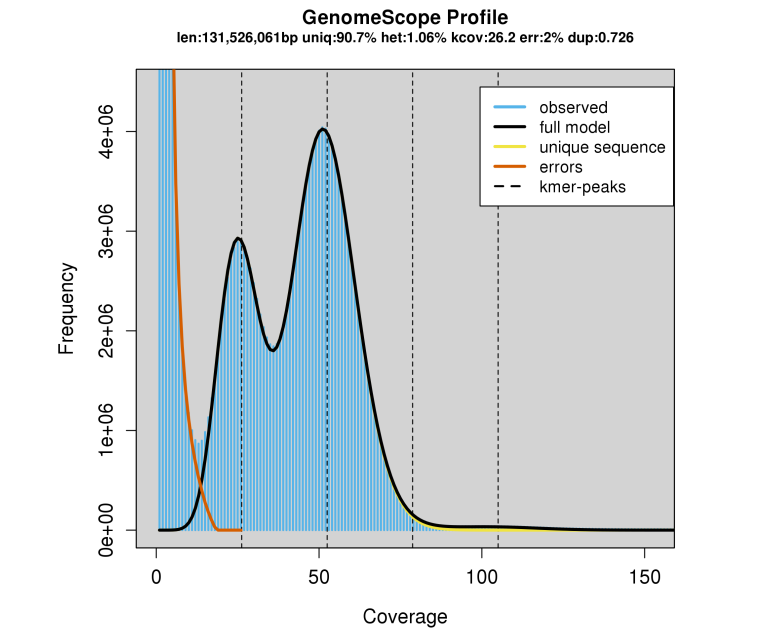
\includegraphics[width=0.6\textwidth]{capitoli/metodi analizzati/genomescope/gnmscp_genomescopeprofile.png}
		\caption{Modello del k-mer profile generato dal programma. L'istogramma in azzurro rappresenta i dati del k-mer profile reale, la curva nera il modello stimato e quella color arancione gli errori di sequenziamento stimati.}
		\label{fig:gnmscp_genomescopeprofile}
	\end{figure}

	\subsection{Gestione degli errori di sequenziamento}
	Eventuali errori di sequenziamento, ad esempio dovuti a duplicazioni con PCR o a sequenze contaminate, sono determinati solo empiricamente: dopo varie iterazioni del software in cui viene abbassata la soglia di copertura richiesta, i k-mer che non riescono ad essere rappresentati dal modello vengono identificati come errori di sequenziamento. 
	
	La stima dei k-mer sequenziati in modo errato è importante perché viene utilizzata per determinare la percentuale di basi errate nelle letture: una singola base inesatta infatti può dar luogo fino a $k$ k-mer errati, aumentando notevolmente il numero di errori. GenomeScope permette una percentuale $e$ di basi errate in ciascun k-mer. Tale valore è calcolato con un fitting dei k-mer errati a una distribuzione binomiale tramite la funzione \verb|uniroot| del linguaggio di programmazione \textit{R}. Questo metodo permette al programma di non dover assumere che la distribuzione degli errori di sequenziamento abbia una particolare forma, né di utilizzare un valore di soglia.
	
\end{document}
	\documentclass[crop=false, class=book]{standalone}

\begin{document}
	\section{findGSE}
	\label{sec:findGSE}
	Il programma \textit{findGSE}~\cite{sun2017findGSE} ha come obiettivo principale la stima della lunghezza del genoma. Utilizzando le frequenze dei k-mer trovati nelle letture a disposizione, il programma compie una regressione non lineare dei dati utilizzando come funzione una \gls{snd} (\textit{skew normal distribution}~\cite{azzalini1985class,azzalini2005skew}).
	
	\subsection{Algoritmo}
	Nel programma viene assunto che le frequenze dei k-mer possano essere approssimate da una \gls{snd} $Y \sim \mathcal{SN}(\xi, \omega^2, \alpha)$. Presa in input la distribuzione delle frequenze dei k-mer (k-mer profile), l'algoritmo effettua la regressione determinando i quattro parametri che descrivono una \gls{snd}, la media $\xi$, la deviazione standard $\omega$, l'asimmetria $\alpha$ e un fattore di scala $s$. Ad ogni iterazione, il programma cerca di minimizzare l'errore tra i dati di input e la funzione stimata, in modo da approssimare il più possibile il k-mer profile reale. La figura~\vref{fig:findGSEfitting} mostra come viene effettuato iterativamente il \gls{fitting} del k-mer profile utilizzando come funzione la suddetta distribuzione.
	
	\begin{figure}[h]
		\centering
		\subfloat[][\emph{Primo \gls{fitting} dei dati dalle letture di input.}]
		{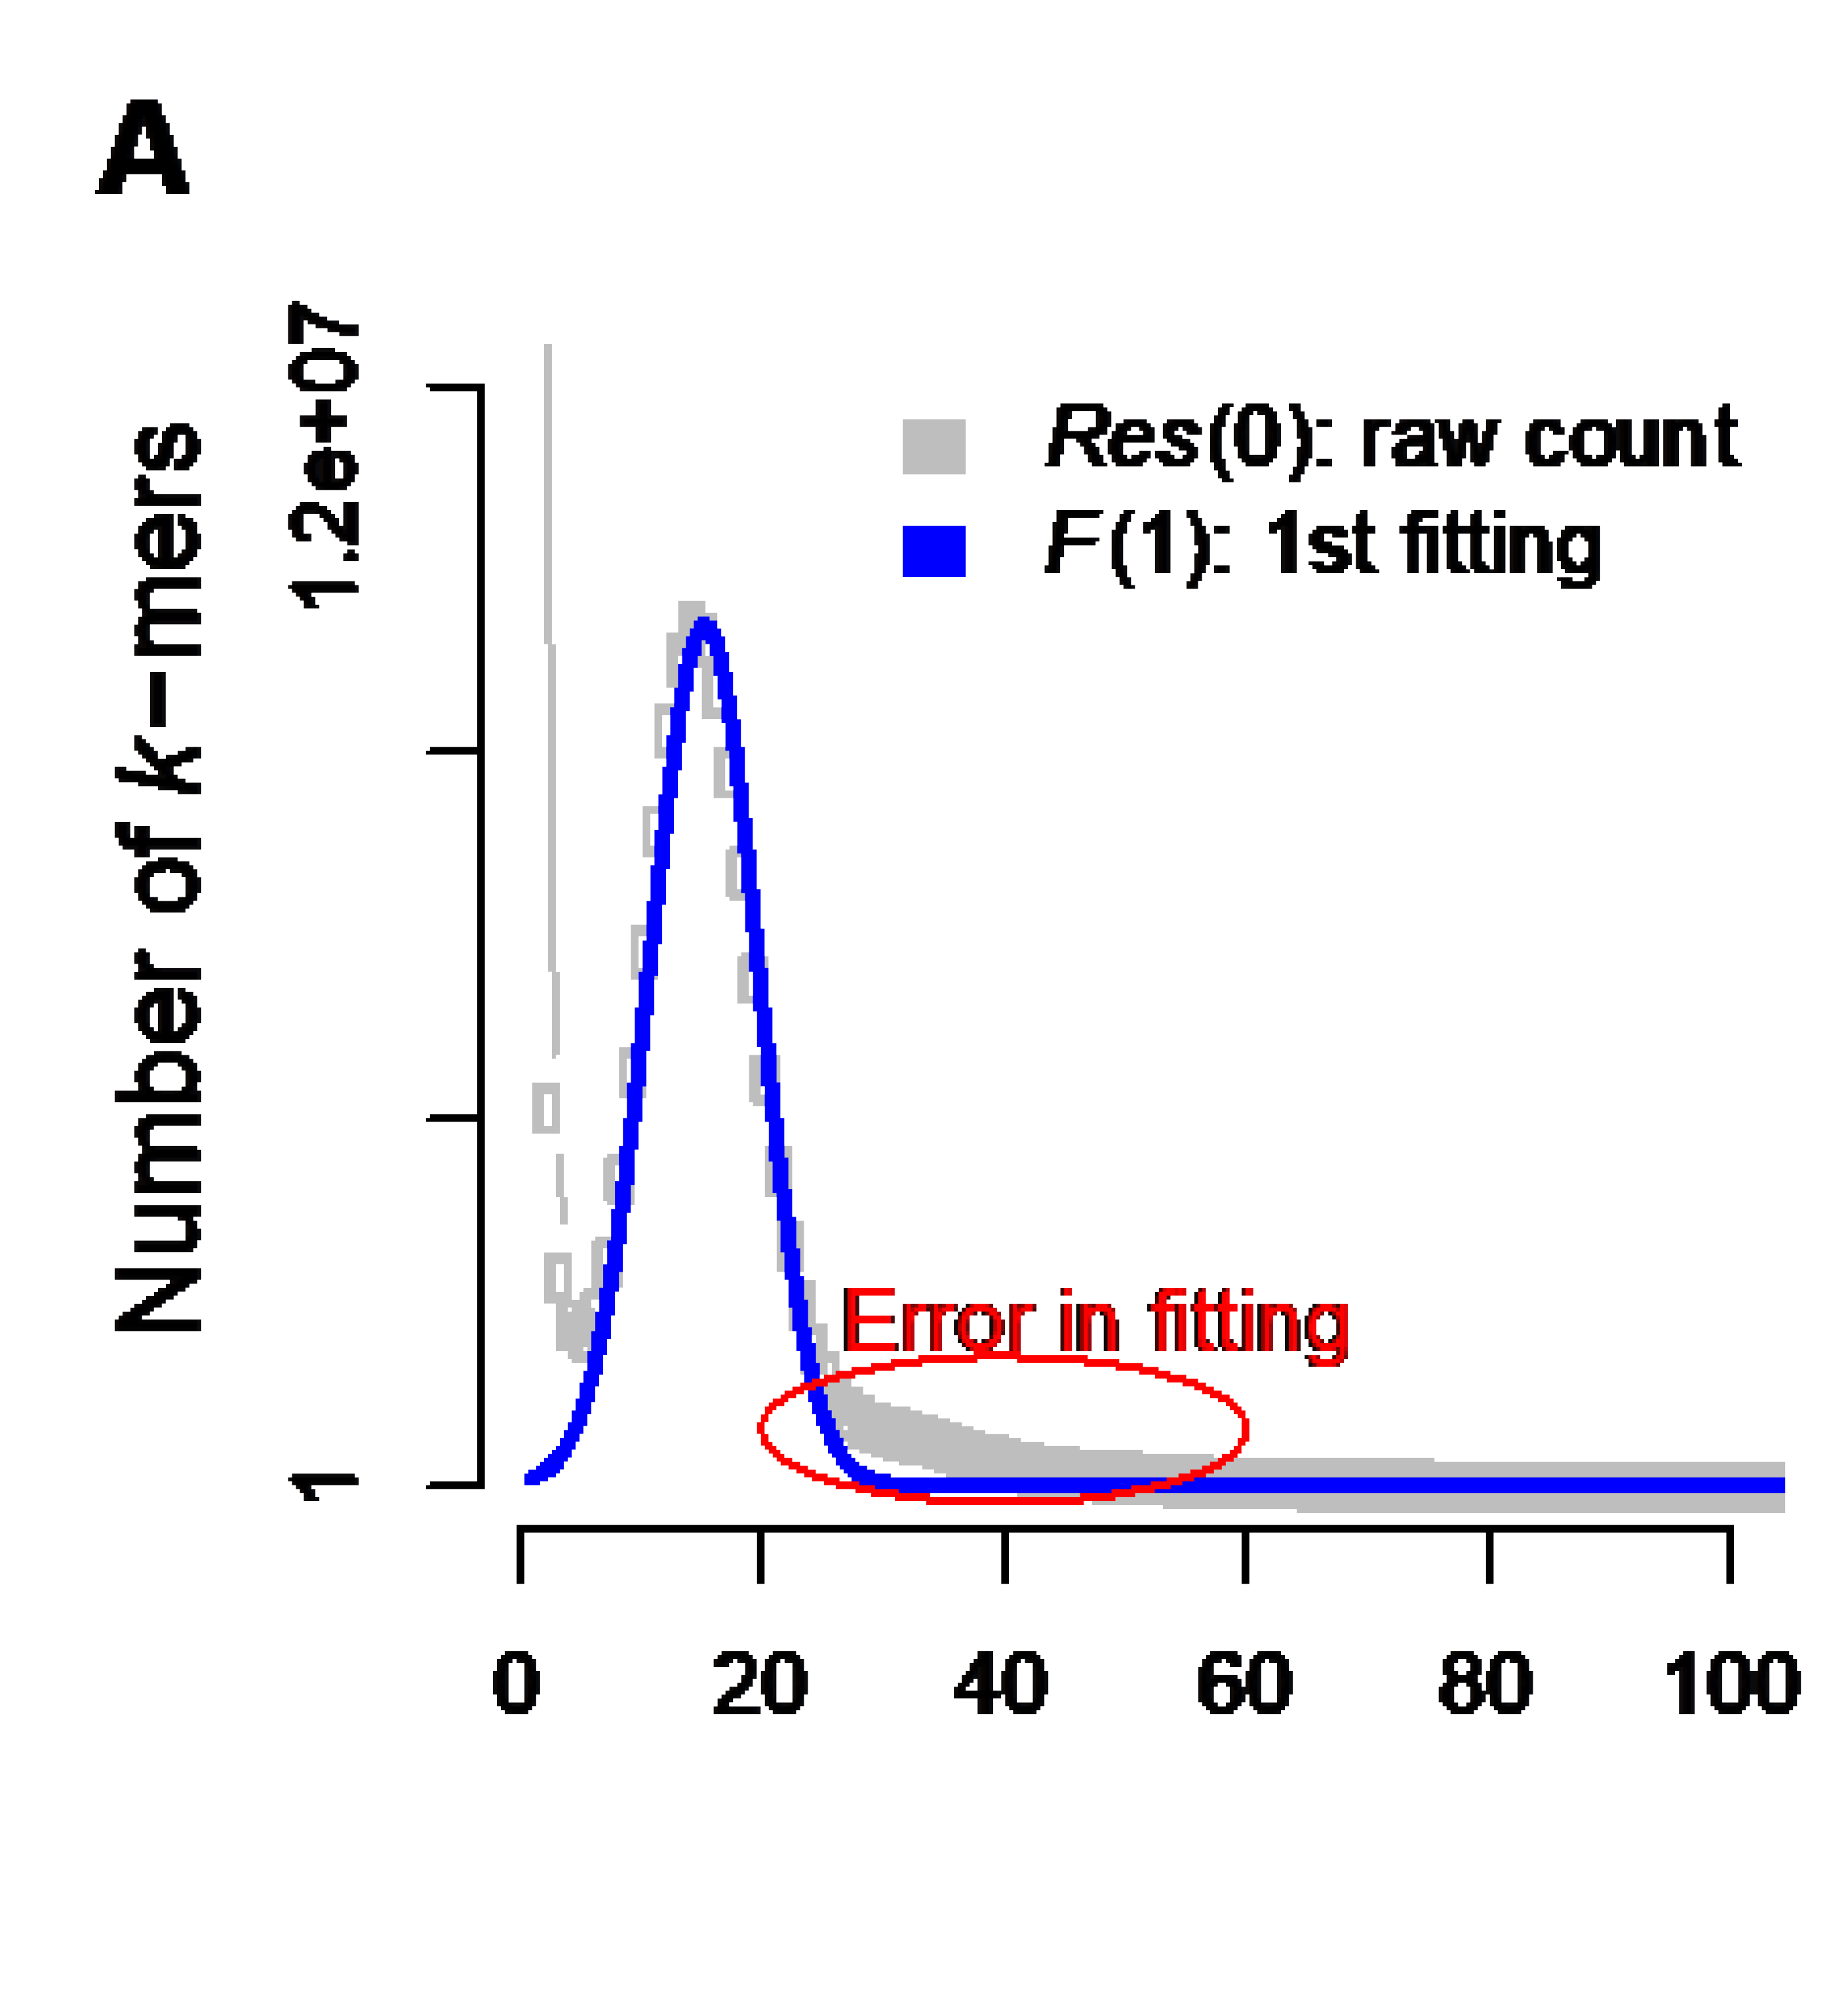
\includegraphics[width=0.31\textwidth]{capitoli/metodi analizzati/findGSE/fittingA.png}} \quad
		\subfloat[][\emph{Secondo \gls{fitting}, utilizzando anche i k-mer residui dalla precedente operazione.}]
		{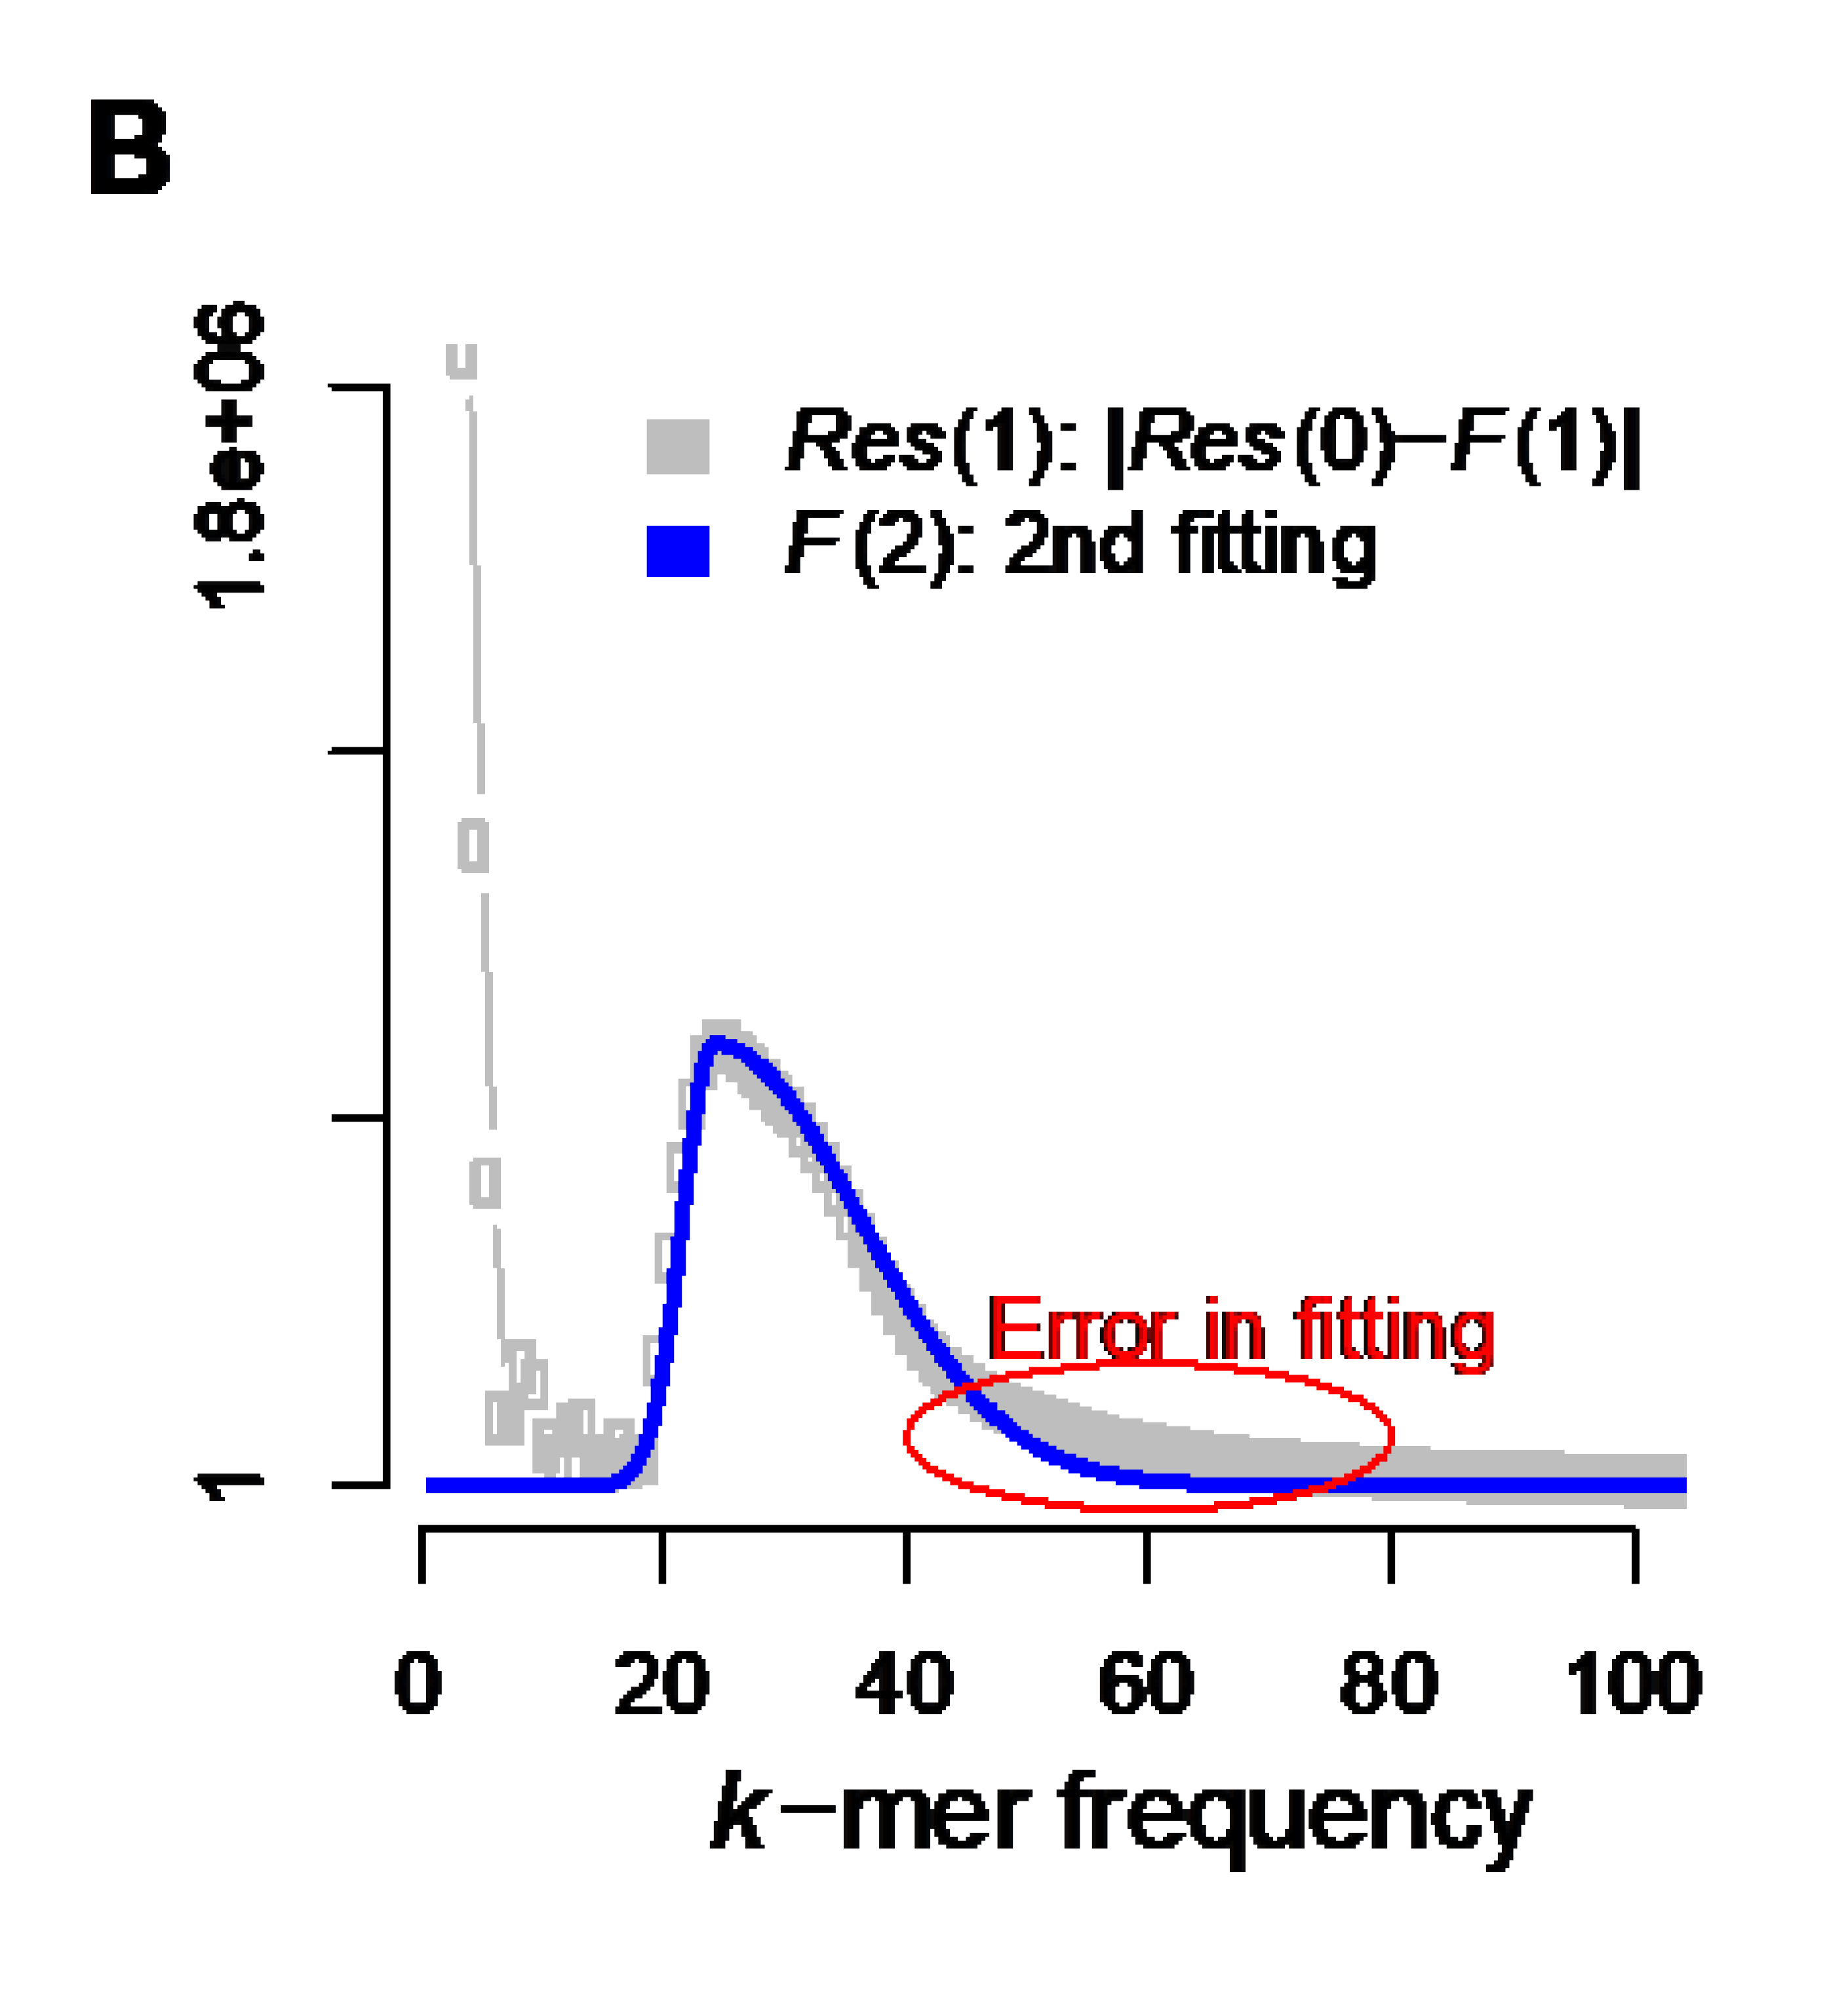
\includegraphics[width=0.31\textwidth]{capitoli/metodi analizzati/findGSE/fittingB.png}} \quad
		\subfloat[][\emph{\gls{fitting} finale.}]
		{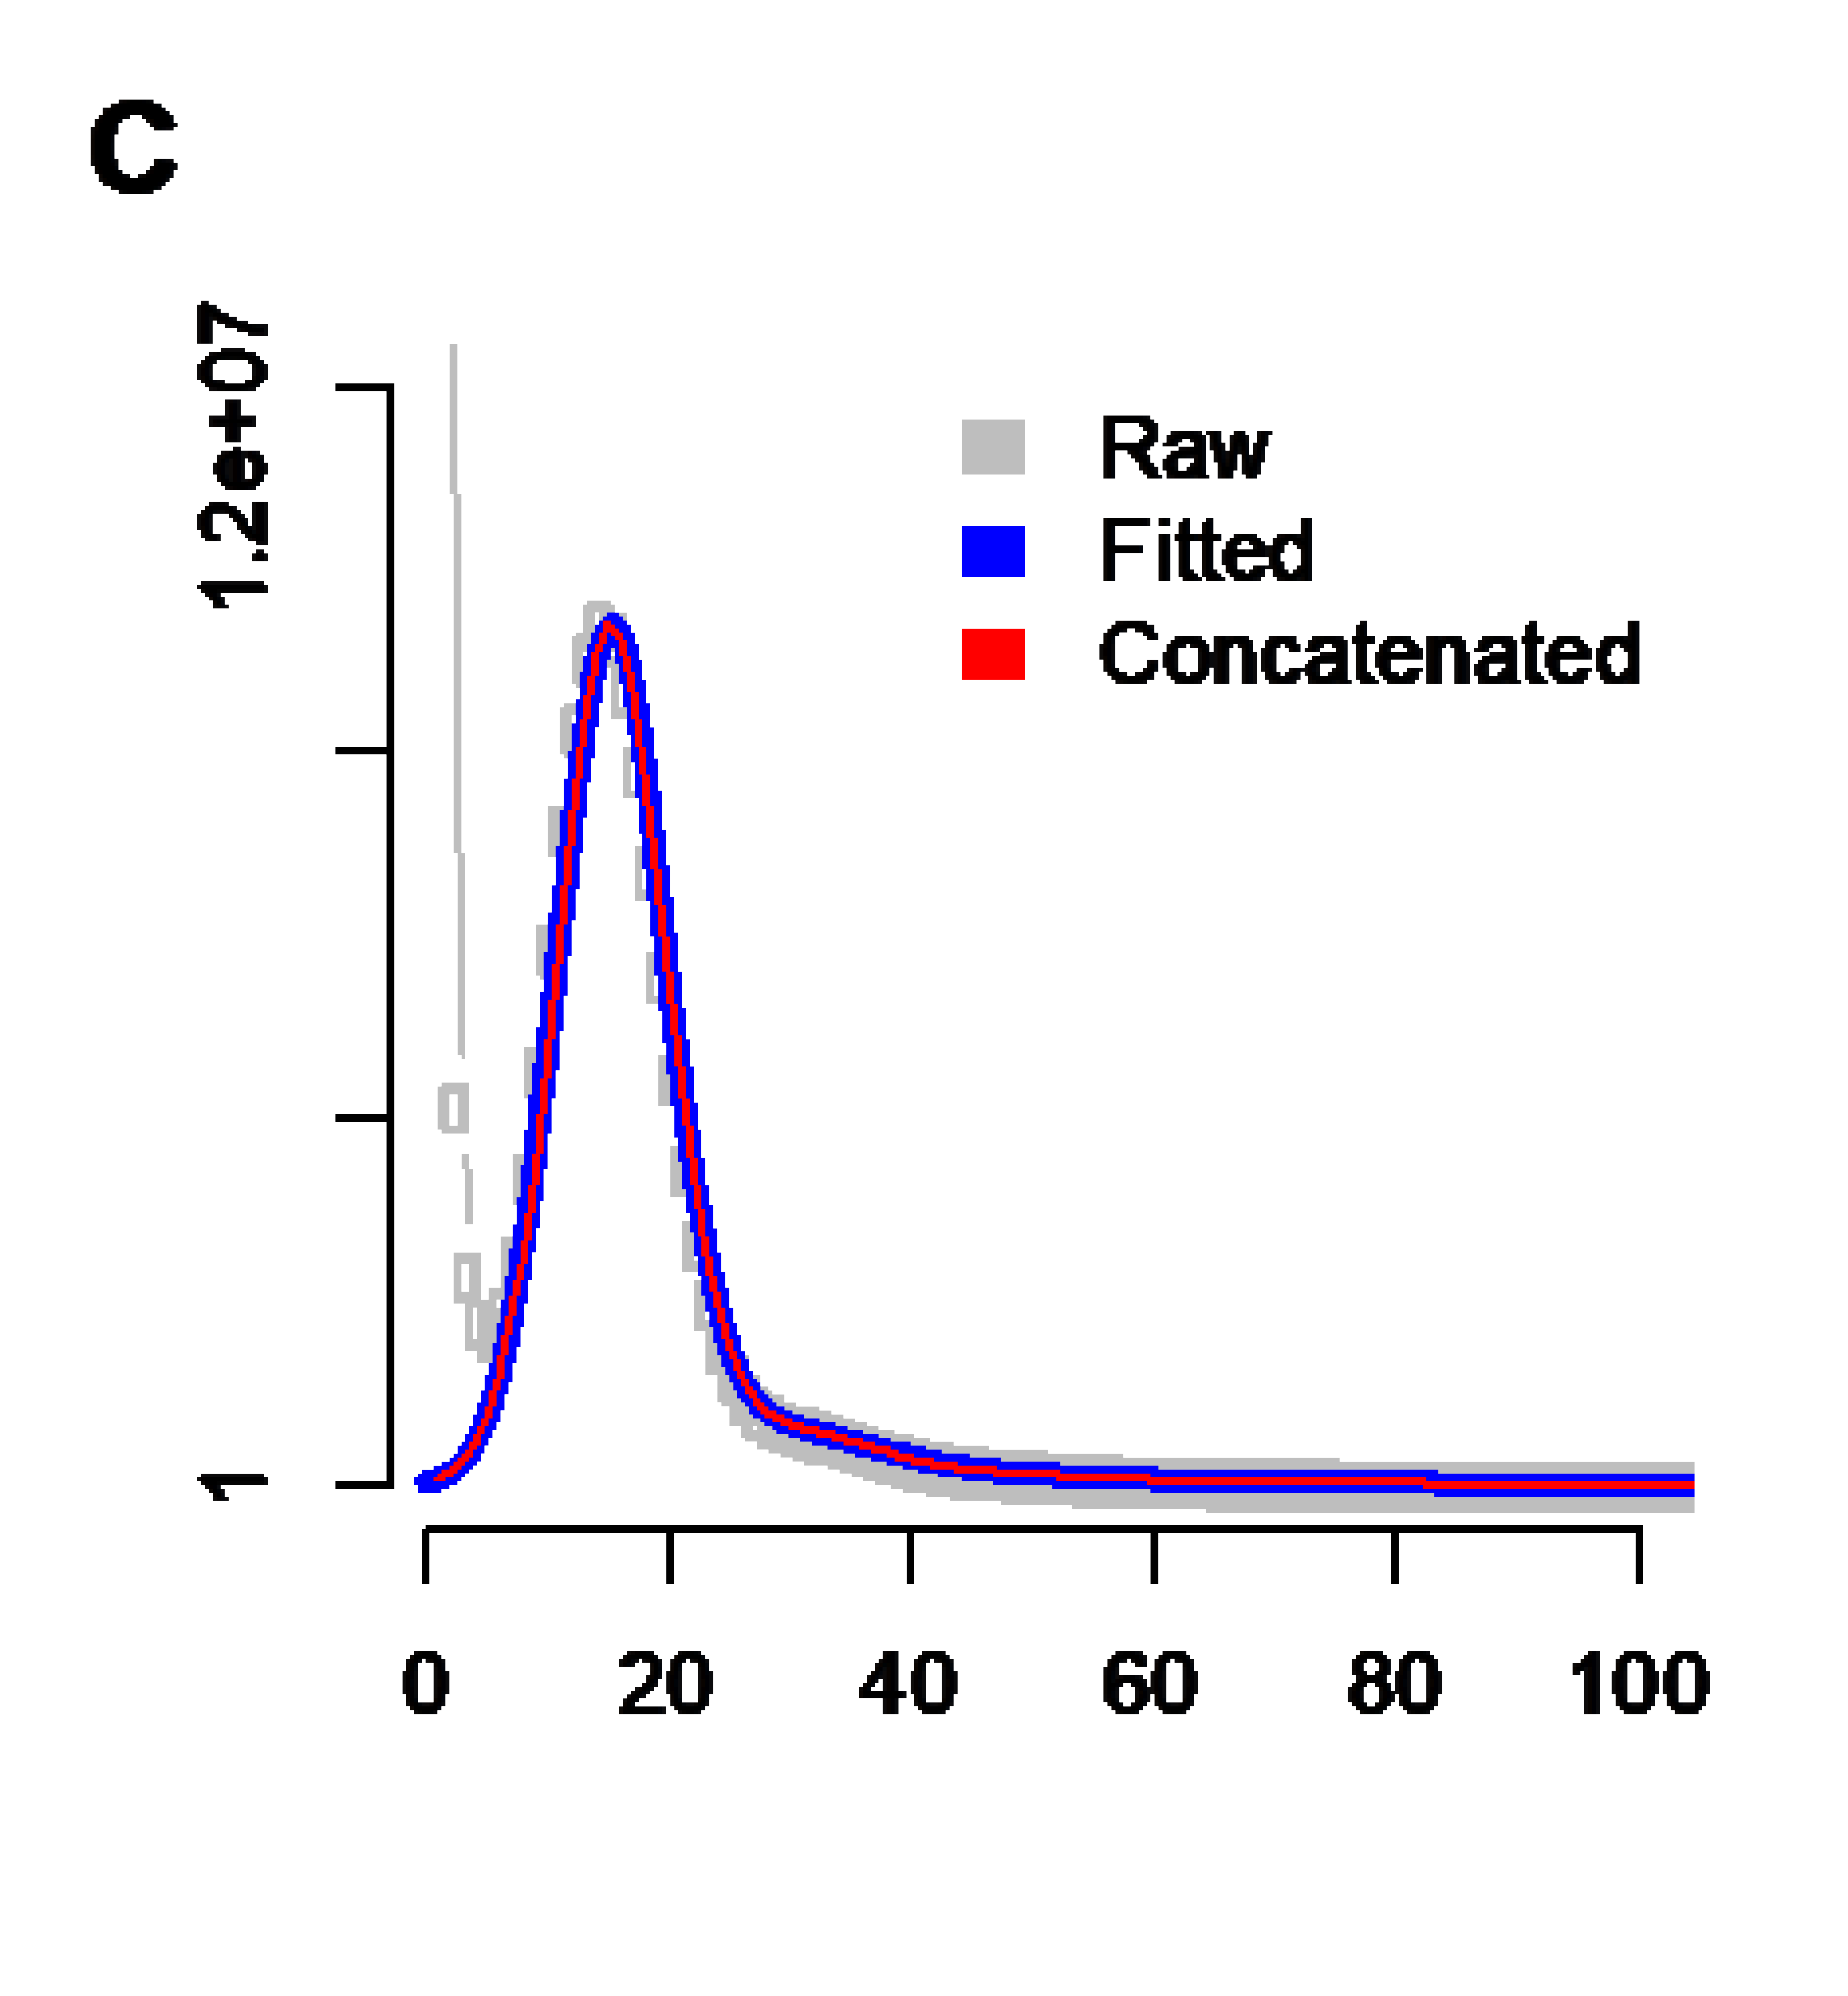
\includegraphics[width=0.31\textwidth]{capitoli/metodi analizzati/findGSE/fittingC.png}} 
		\caption{Esempio di \gls{fitting} iterativo del k-mer profile.}
		\label{fig:findGSEfitting}
	\end{figure}

	Dato un genoma aploide con $G$ basi, il numero di k-mer possibili sarà $G-k+1$. Ponendo $C$ la copertura media dei k-mer, in modo che in media ogni k-mer sia trovato in $C$ letture diverse, e $N$ il numero di k-mer trovati nelle letture, la quantità di k-mer presenti nel genoma è descritta dall'equazione~\vref{eqn:findGSE1}. 	
	
	\begin{equation}
		\label{eqn:findGSE1}
		N=C \times (G-K+1).
	\end{equation}
		
	Posta la dimensione del genoma molto maggiore del numero di basi utilizzate $G\gg k$, l'equazione~\vref{eqn:findGSE2} approssima la dimensione totale del genoma in analisi.
	
	\begin{equation}
		\label{eqn:findGSE2}
		G\approx N/C.
	\end{equation}

	A partire sia dal profilo reale che dal modello stimato, il programma calcola quindi il numero totale di k-mer trovati $N$ e la copertura media dei k-mer $C$, per poi calcolare la dimensione del genoma attraverso l'equazione~\vref{eqn:findGSE2}.
	
	\subsection{Analisi di genomi reali}
	Utilizzando letture reali, i dati devono essere precedentemente processati per minimizzare gli errori di stima del genoma. Per questo è consigliabile ridurre prima le letture con il programma \textit{Skewer}~\cite{jiang2014skewer}, ed eliminare quelle con lunghezza minore di 33 bp. Per ottenere risultati migliori, inoltre, è consigliabile rimuovere le letture doppie dovute alla duplicazione PCR tramite il programma \textit{FastUniq}~\cite{xu2012fastuniq}, e le sequenze di simili a DNA dei mitocondri o dei cloroplasti con i programmi \textit{BWA}~\cite{li2009fast} e \textit{SAMtools}~\cite{li2009sequence}.
	
\end{document}
	\documentclass[crop=false, class=book]{standalone}

\begin{document}
	\section{MGSE}
	\label{sec:MGSE}
	Il programma \textit{Mapping-based Genome Size Estimation} (\textit{MGSE}) stima la dimensione del genoma attraverso il calcolo della copertura media a partire dall'assembly ad alta contiguità delle letture~\cite{pucker2019MGSE}. Lo script è open-source e scritto in Python, e processa le informazioni sulla copertura delle letture di input restituendo la dimensione stimata del genoma.
	
	\subsection{Algoritmo}
	Posto che le letture di input siano distribuite equamente sull'intera sequenza del genoma, il programma ne stima la dimensione calcolandone la copertura media. Se infatti sono noti il numero $L$ di basi sequenziate e la copertura $C$ in una certa posizione, la lunghezza totale $N$ del genoma sarà pari a $N = L/C$.
	
	Dato che le letture non forniscono la stessa copertura in tutte le regioni, ad esempio a causa di sequenze ripetitive, per una stima reale della dimensione del genoma è importante un calcolo corretto della copertura media. Per questo, il programma permette all'utente di inserire una lista di regioni di riferimento usate per il calcolo della media e della mediana della copertura. A questo scopo può essere utile il programma \textit{Benchmarking Universal Single Copy Orthologs} (\textit{BUSCO})~\cite{simao2015busco}, che identifica un gruppo di sequenze \textit{bona fidae}, cioè che sono a singola copia e che hanno solo una sola corrispondenza all'interno del genoma~\cite{li2005trumatch}, le quali possono risultare adatte al calcolo della copertura media. 
	
	Il programma per poter effettuare la stima della dimensione del genoma riceve in input un file contenente la versione binaria compressa di sequenze allineate (file \textit{bam}~\cite{li2009sequence}), oppure un file contenente informazioni sulla copertura per ogni porzione della sequenza da sequenziare (file \textit{cov}~\cite{pucker2018genome}). Dopo aver calcolato la media e la mediana della copertura, il programma produce in output le dimensioni del genoma stimate per entrambi i valori.
	
\end{document}
	
	% Capitolo 3
	\documentclass[crop=false, class=book]{standalone}

\usepackage{lipsum}

\begin{document}
	
	\chapter{Valutazione dei metodi}
	In questo capitolo viene eseguita l'analisi di ciascun metodo, a partire dalla propria complessità e dalla precisione dimostrata. Vengono poi presentate due serie di confronti tra alcuni dei programmi analizzati, per cercare di determinare quale sia il migliore.
	
	
\end{document}
	\documentclass[crop=false, class=book]{standalone}

\begin{document}
	
	\section{Complessità e performance}
	In questo paragrafo vengono analizzate per ciscun metodo la complessità, i requisiti richiesti per l'esecuzione e l'accuratezza dimostrata nei test eseguiti da ciascun gruppo di ricerca. Si noti che la misurazione fatta del numero di righe per ciascun programma considera solo il codice sorgente, escludendo gli spazi bianchi e i commenti.
	
	
	\subsection{ALLPATHS-LG}
	Dato che il programma ha come obiettivo principale l'assembly delle letture di input, esso presenta una complessità elevata (984 file, 209677 righe di codice). Inoltre, per far sì che il programma possa gestire genomi di grandi dimensioni, si rende necessario l'utilizzo di dispositivi server commerciali, in modo da svolgere l'elaborazione mantenendo in memoria grandi quantità di dati. Per esempio, l'assembly del genoma di un mammifero può essere fatto in alcune settimane utilizzando un server \textit{Dell~R815} con 48 processori e 512 GB di memoria RAM disponibile \cite{gnerre2011high}. Altri metodi di sequenziamento tramite de novo assembly, come ad esempio il programma \mbox{\textit{SOAPdenovo}}~\cite{li2010denovo}, riescono a completare l'assembly in un tempo minore a parità di dati in input e di risorse computazionali disponibili. Nonostante ciò, utilizzando letture di dimensioni minori ma a maggiore copertura, ALLPATHS-LG produce assembly di qualità più elevata rispetto agli altri programmi.
	
	Il metodo, essendo molto più complesso e richiedendo maggiori capacità computazionali rispetto agli altri programmi analizzati, può risultare sovradimensionato per la sola stima della dimensione del genoma. Il valore stimato dal software, tuttavia, può risultare utile nel confronto con gli altri metodi.
	
	\subsection{GCE}
	Il programma presenta una complessità media (1150 righe di codice) e permette di stimare la dimensione del genoma tramite uno dei modelli descritti nel paragrafo~\vref{sec:GCE} in base al genoma che si deve analizzare, come ad esempio i modelli omozigote o eterozigote, continuo o discreto.
	
	Considerando come genomi di riferimento altri progetti di sequenziamento tramite de novo assembly, come quello dell'E.\  coli-O104:H4~\cite{li2011genomic}, della formica tagliafoglie~\cite{nygaard2011genome}, della patata~\cite{xu2011genome} o del panda~\cite{li2010sequence}, le dimensioni stimate dal programma utilizzando dati simulati dimostrano un'elevata accuratezza. 
	
	Nella stima di genomi reali invece, dovendo eseguire un filtraggio e una correzione degli errori sui dati originali per diminuire la complessità della computazione e, quindi, il consumo di memoria, si registra una diminuzione della precisione~\cite{liu2013GCE}. Il valore dedotto dal programma, comunque, può risultare utile per determinare la strategia di sequenziamento di un genoma, e per guidare lo sviluppo di algoritmi per l'assembly. 
	
	
	\subsection{GenomeScope}
	GenomeScope risulta un programma veloce, dal momento che processa i dati in meno di un minuto con consumi non eccessivi di memoria RAM, e mostrando una complessità media (501 righe di codice). Il programma, inoltre, restituisce in output un file testuale contenente le proprietà del genoma analizzato, oltre a immagini in alta qualità del modello costruito~\cite{vurture2017genomescope}.
	
	Nei test eseguiti dal gruppo di ricerca, il programma ha dimostrato un'alta affidabilità: sia nella valutazione di dati simulati di vari organismi variando il \gls{rate_eterozigosity}, il rapporto di duplicazione, la copertura e il numero di errori di sequenziamento, sia sulla stima di genomi reali combinati sinteticamente, il metodo riscontra una buona approssimazione delle caratteristiche delle sequenze. Nell'analisi di dati reali invece, si riscontra una precisione del 99,7\% rispetto alle stime fatte con altri metodi, come genomi di riferimento o \textit{flow cytometry}. 

	Per la maggior parte dei casi viene consigliato l'utilizzo di k-mer con valore $k = 21$, che può essere aumentato per genomi con dimensioni molto elevate (dimensione aploide~$\gg$~10~Gb) o che presentano un elevato numero di sequenze ripetitive. Una scarsa copertura (in genere, minore di $25\times$) o un elevato rapporto di errore di sequenziamento, inoltre, potrebbero impedire al modello di convergere con il k-mer profile reale. La flessibilità del programma nel numero di distribuzioni utilizzate per il \gls{fitting}, infine, potrebbe risultare adeguata anche per lo studio di genomi poliploidi, che al momento risultano difficilmente trattabili~\cite{sun2017findGSE}.

	
	\subsection{findGSE}
	Il programma findGSE, che esegue il \gls{fitting} di una \gls{snd} al k-mer profile, presenta una complessità media (969 righe di codice) e permette la stima della dimensione del genoma utilizzando risorse modeste. 
	
	Nell'analisi di genomi simulati la stima avviene quasi perfettamente, anche applicando variazioni al rapporto di errore di sequenziamento, alla copertura o al livello di eterozigosi. Il valore della stima della dimensione del genoma di \textit{Arabidopsis thaliana} generata dal programma si dimostra leggermente minore al valore trovato tramite il metodo \textit{flow cytometry}, con il quale comunque condivide una forte correlazione~\cite{sun2017findGSE}. 
	
	Il programma è stato utilizzato anche per la stima della dimensione di genoma umano. Prendendo come riferimento la versione GRCh38.p9 sviluppata da \textit{The Genome Reference Consortium}, il programma ha riscontrato una differenza di 41 Mb tra i genomi maschile e femminile, similmente alla differenza di 49 Mb tra i due sessi del genoma di riferimento.
	
	\subsection{MGSE}
	MGSE presenta una complessità minore rispetto agli altri programmi presentati (323 righe di codice), e raggiunge le prestazioni migliori con assembly ad alta contiguità~\cite{pucker2019MGSE}. Rispetto alla maggior parte degli altri metodi basati sui k-mer, esso richiede un genoma di riferimento per il calcolo della copertura media, come ad esempio le sequenze individuate dal software \textit{BUSCO}. 
	
	Il programma, se l'assembly include tutte le regioni a singola copia e almeno un'occorrenza di quelle ripetitive, si dimostra affidabile. Esso permette inoltre di gestire le regioni contenenti DNA affetto da contaminazioni batteriche o fungine, nel caso in cui esse non siano incluse nelle sequenze di riferimento, procedendo con l'esclusione delle letture corrispondenti. 
	
	Invece, nel caso in cui solo alcune sequenze di input siano state duplicate tramite PCR, risulta impossibile distinguere tali copie dalle sequenze presenti nel genoma reale in più di una regione. Il programma comunque prevede una certa tolleranza se la duplicazione è stata fatta equamente su tutte le letture di input.


	
\end{document}
	\documentclass[crop=false, class=book]{standalone}

\begin{document}
	
	\section{Confronti tra i metodi}
	In questo paragrafo vengono mostrate due serie di confronti tra alcuni dei metodi presentati. In entrambi i casi a ciascun metodo vengono forniti gli stessi dati di input che, indipendentemente l'uno dall'altro, vengono processati per stimare la dimensione del genoma sotto specifiche condizioni.
	
	\subsection{Metodi findGSE, ALLPATHS-LG, GCE e GenomeScope}
	I dati e le figure della seguente analisi sono state ricavate da \cite{sun2017findGSE}, che esegue un confronto tra i metodi findGSE, ALLPATHS-LG, GCE e GenomeScope.
	Si noti che nelle figure sono inclusi due metodi non trattati in questo documento (\textit{naive} ed \textit{egs}), i cui risultati non saranno pertanto analizzati.
	Il genoma di riferimento utilizzato per l'analisi di letture simulate di \textit{A. thaliana} è una sequenza di circa 119 Mb. 
	
	\paragraph{Variazione della copertura}
	Inizialmente vengono utilizzate letture simulate di un genoma omozigote con copertura minima 50$\times$ e con l'1\% di basi errate nel sequenziamento. Tutti i programmi si dimostrano precisi e stabili, stimando la dimensione del genoma tra 118 e 123 Mb a fronte di un valore reale di 119 Mb, come mostrato dalla figura~\vref{fig:confronto1}. Riducendo gradualmente la copertura da 50$\times$ a 10$\times$, tutti i metodi riportano una stima corretta fino a 30$\times$. Nel caso di una bassa copertura (10$\times$), i metodi ALLPATHS-LG e GenomeScope falliscono nel dare una stima della dimensione del genoma.
	
	\begin{figure}[h]
		\centering
		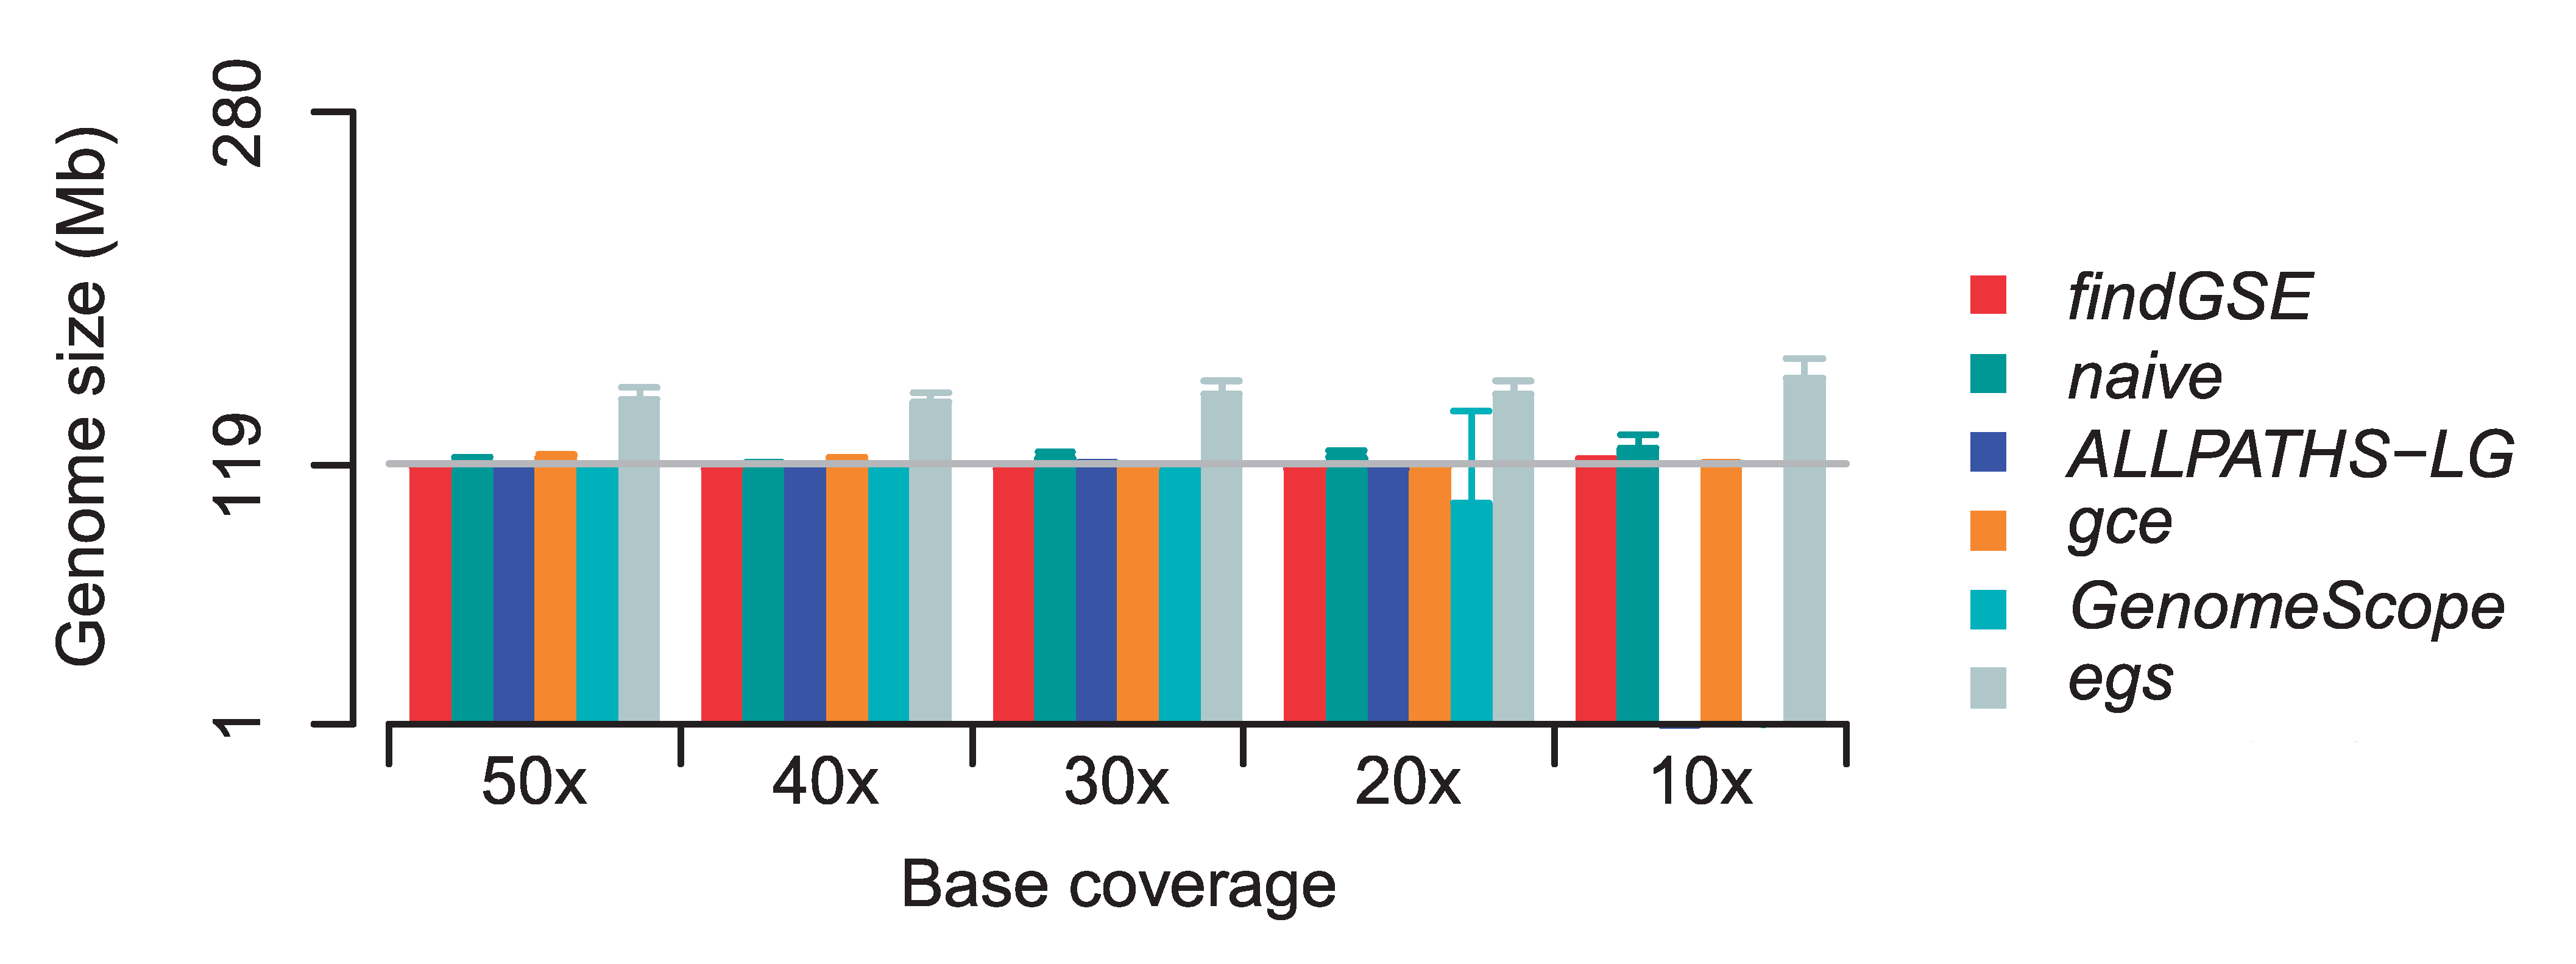
\includegraphics[height=0.21\textheight]{capitoli/analisi/confronto/confronto1/a.png}
		\caption{Stima della dimensione del genoma, con valore di copertura minima variabile.}
		\label{fig:confronto1}
	\end{figure}

	\paragraph{Errori di sequenziamento}
	Modificando invece il rapporto di errore di sequenziamento, i programmi generano risultati quasi sempre compatibili con la grandezza reale, come mostrato dalla figura~\vref{fig:confronto2}. Si noti che con un rapporto di errore elevato e non realistico (5\%), mentre gli altri metodi mantengono la stessa precisione ALLPATHS-LG restituisce un valore instabile.
	
	\begin{figure}
		\centering
		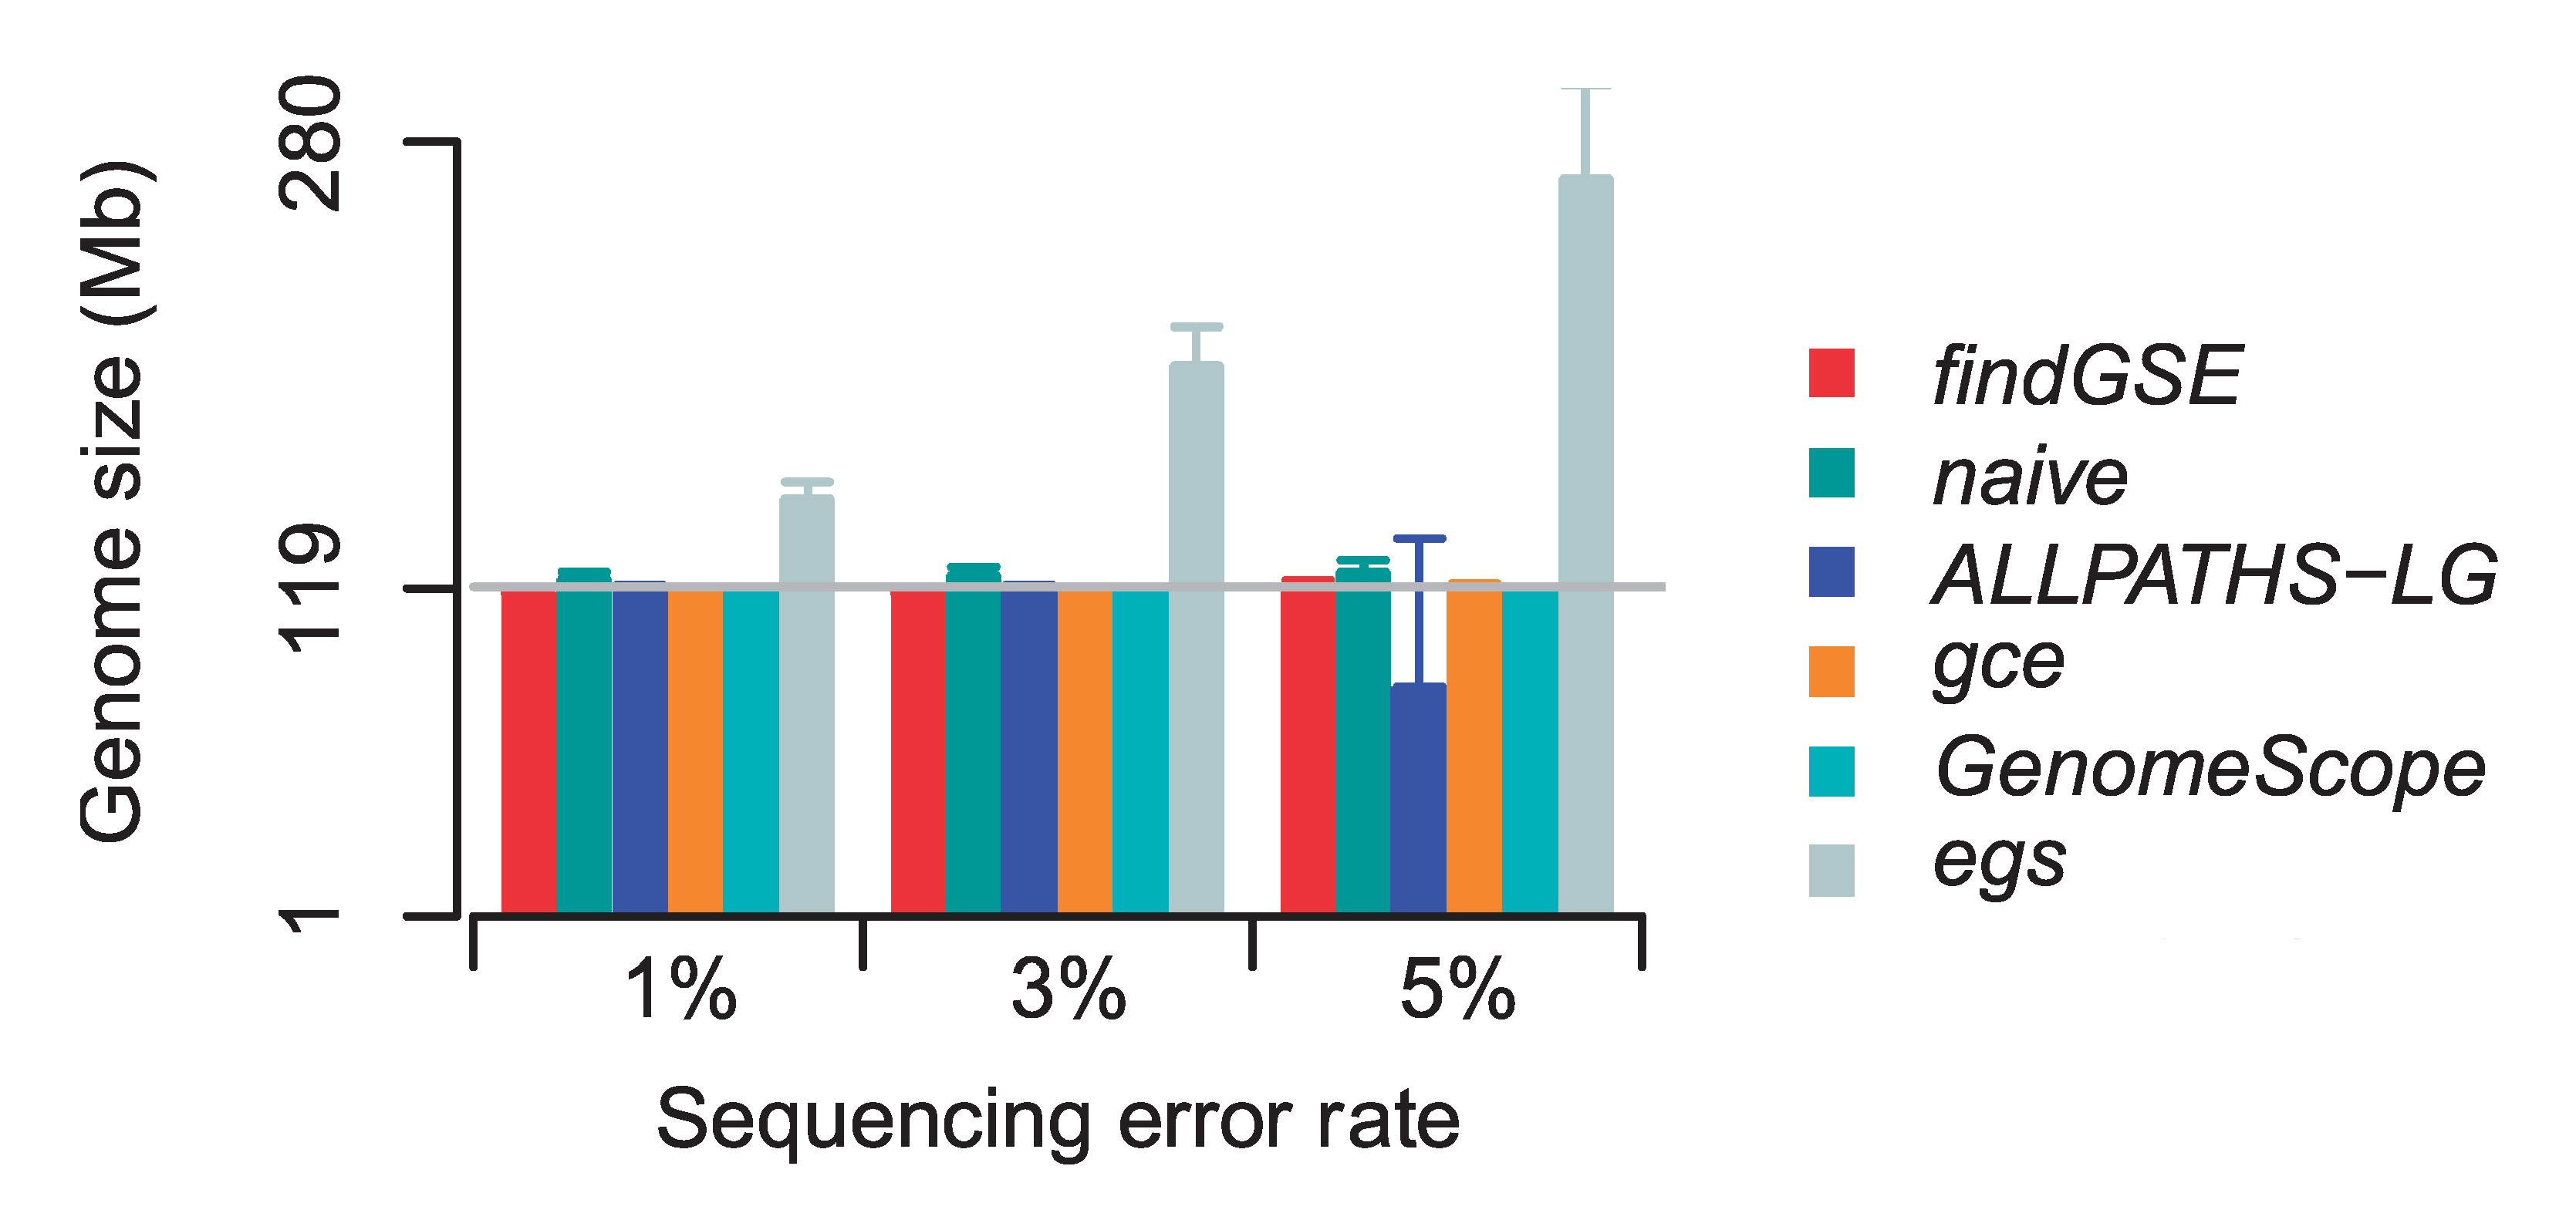
\includegraphics[height=0.21\textheight]{capitoli/analisi/confronto/confronto1/c.png}
		\caption{Stima della dimensione del genoma con tasso di errore di sequenziamento variabile.}
		\label{fig:confronto2}
	\end{figure}

	\paragraph{Influenza dell'eterozigosi}
	Per la valutazione dell'impatto dell'eterozigosi, è stata considerata una sequenza con copertura 30$\times$, un rapporto di errore di sequenziamento dell'1\% e un rapporto di mutazioni \gls{snp} da 0,1 a 5,0\%. Per livelli bassi di eterozigosi (da 0,1 a 1,0\%) tutti i metodi risultano precisi e concordi, come mostrato dalla figura~\ref{fig:confronto3}. 
	
	Aumentando il \gls{rate_eterozigosity} (da 2,0 a 5,0\%), la discrepanza tra i valori predetti e quello reale aumenta considerevolmente: su un totale di 280 stime per metodo infatti, i programmi ALLPATHS-LG e GenomeScope hanno generato valori doppi rispetto alla grandezza reale rispettivamente in 150 e 29 previsioni. Le stime erronee dei due programmi sono dovute all'erronea selezione del picco eterozigote come se fosse quello omozigote, che porta a un calcolo non corretto della copertura e quindi al raddoppio della dimensione totale stimata. Gli stessi metodi hanno riportato valori nulli o estremamente bassi rispettivamente in 110 e 173 casi, generando quindi in totale valori erronei con probabilità del 92,9\% per \mbox{ALLPATHS-LG} e del 72,1\% per \mbox{GenomeScope}. 
	Anche nel caso del metodo GCE, un alto tasso di eterozigosi fa generare al programma 120 valori errati su 280 totali, cioè nel 42,9\% delle predizioni. 
	Il metodo findGSE si dimostra poco influenzato dall'aumento del \gls{rate_eterozigosity}, che nel peggiore dei casi fa sovrastimare di poco la dimensione del genoma \mbox{(125 $\pm$ 7 Mb)}.
 
 	\begin{figure}
 		\centering
 		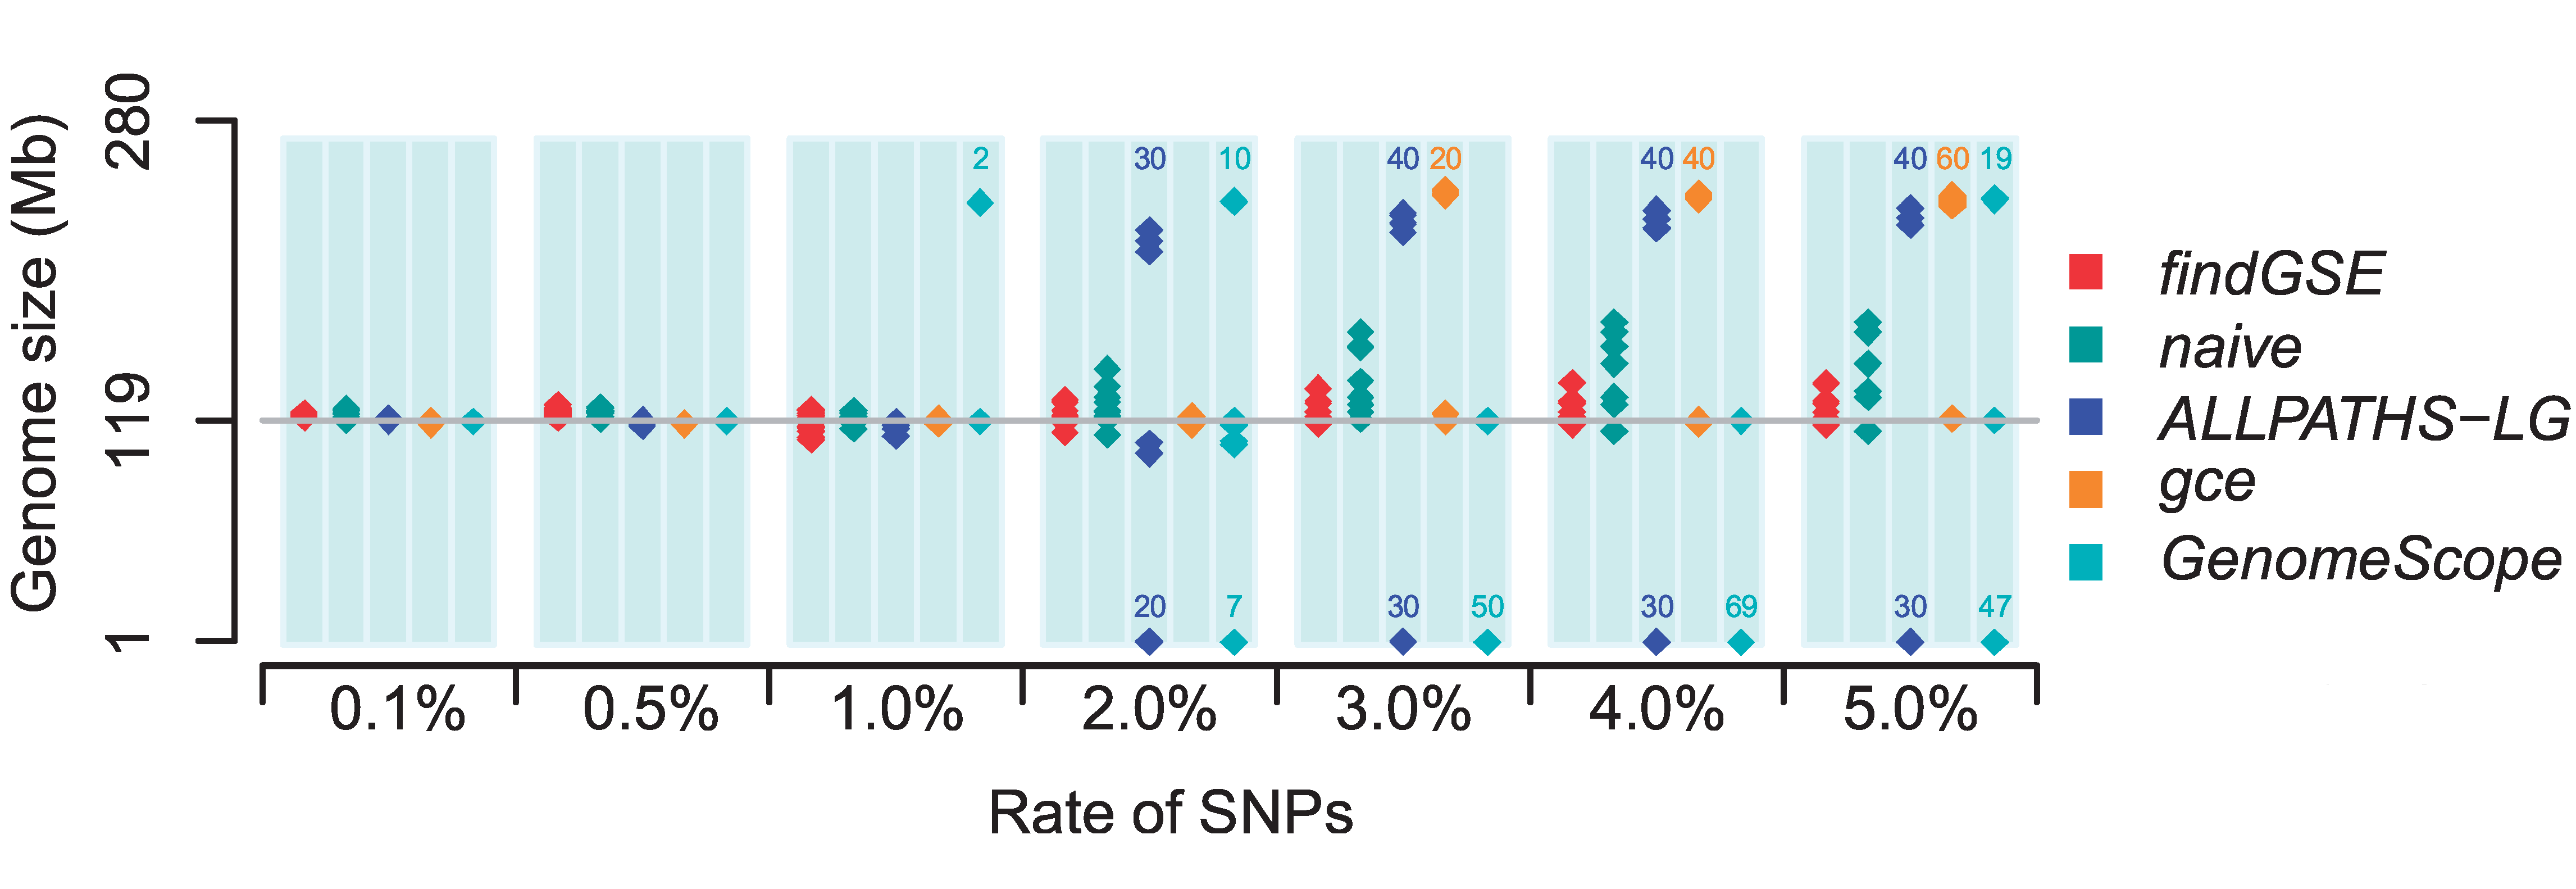
\includegraphics[height=0.21\textheight]{capitoli/analisi/confronto/confronto1/d.png}
 		\caption{Stima della dimensione del genoma con livello di eterozigosi variabile e copertura base 30$\times$. Si noti che i valori rappresentati indicano il numero di punti sovrapposti in una certa regione.}
 		\label{fig:confronto3}
 	\end{figure}
 
 	Mantenendo elevato il tasso di errore di sequenziamento, l'aumento della copertura minima a 100$\times$ (figura~\ref{fig:confronto4}) diminuisce il numero di stime non corrette per i metodi ALLPATHS-LG e GenomeScope, generando rispettivamente 60 (21,4\%) e 110 (39,3\%) valori errati. 
 	Il programma GCE invece, anche all'aumentare della copertura produce molti risultati errati, 210 su 280 totali (75\%).
 	Il metodo findGSE infine si dimostra molto accurato anche ad un alto \gls{rate_eterozigosity}, stimando una dimensione media di \mbox{121 $\pm$ 1 Mb}. 
 	Il programma GenomeScope, tralasciando il problema di duplicazione della dimensione, si dimostra quello con i risultati più stabili tra i  metodi analizzati.
 	
	 \begin{figure} 
	 	\centering
	 	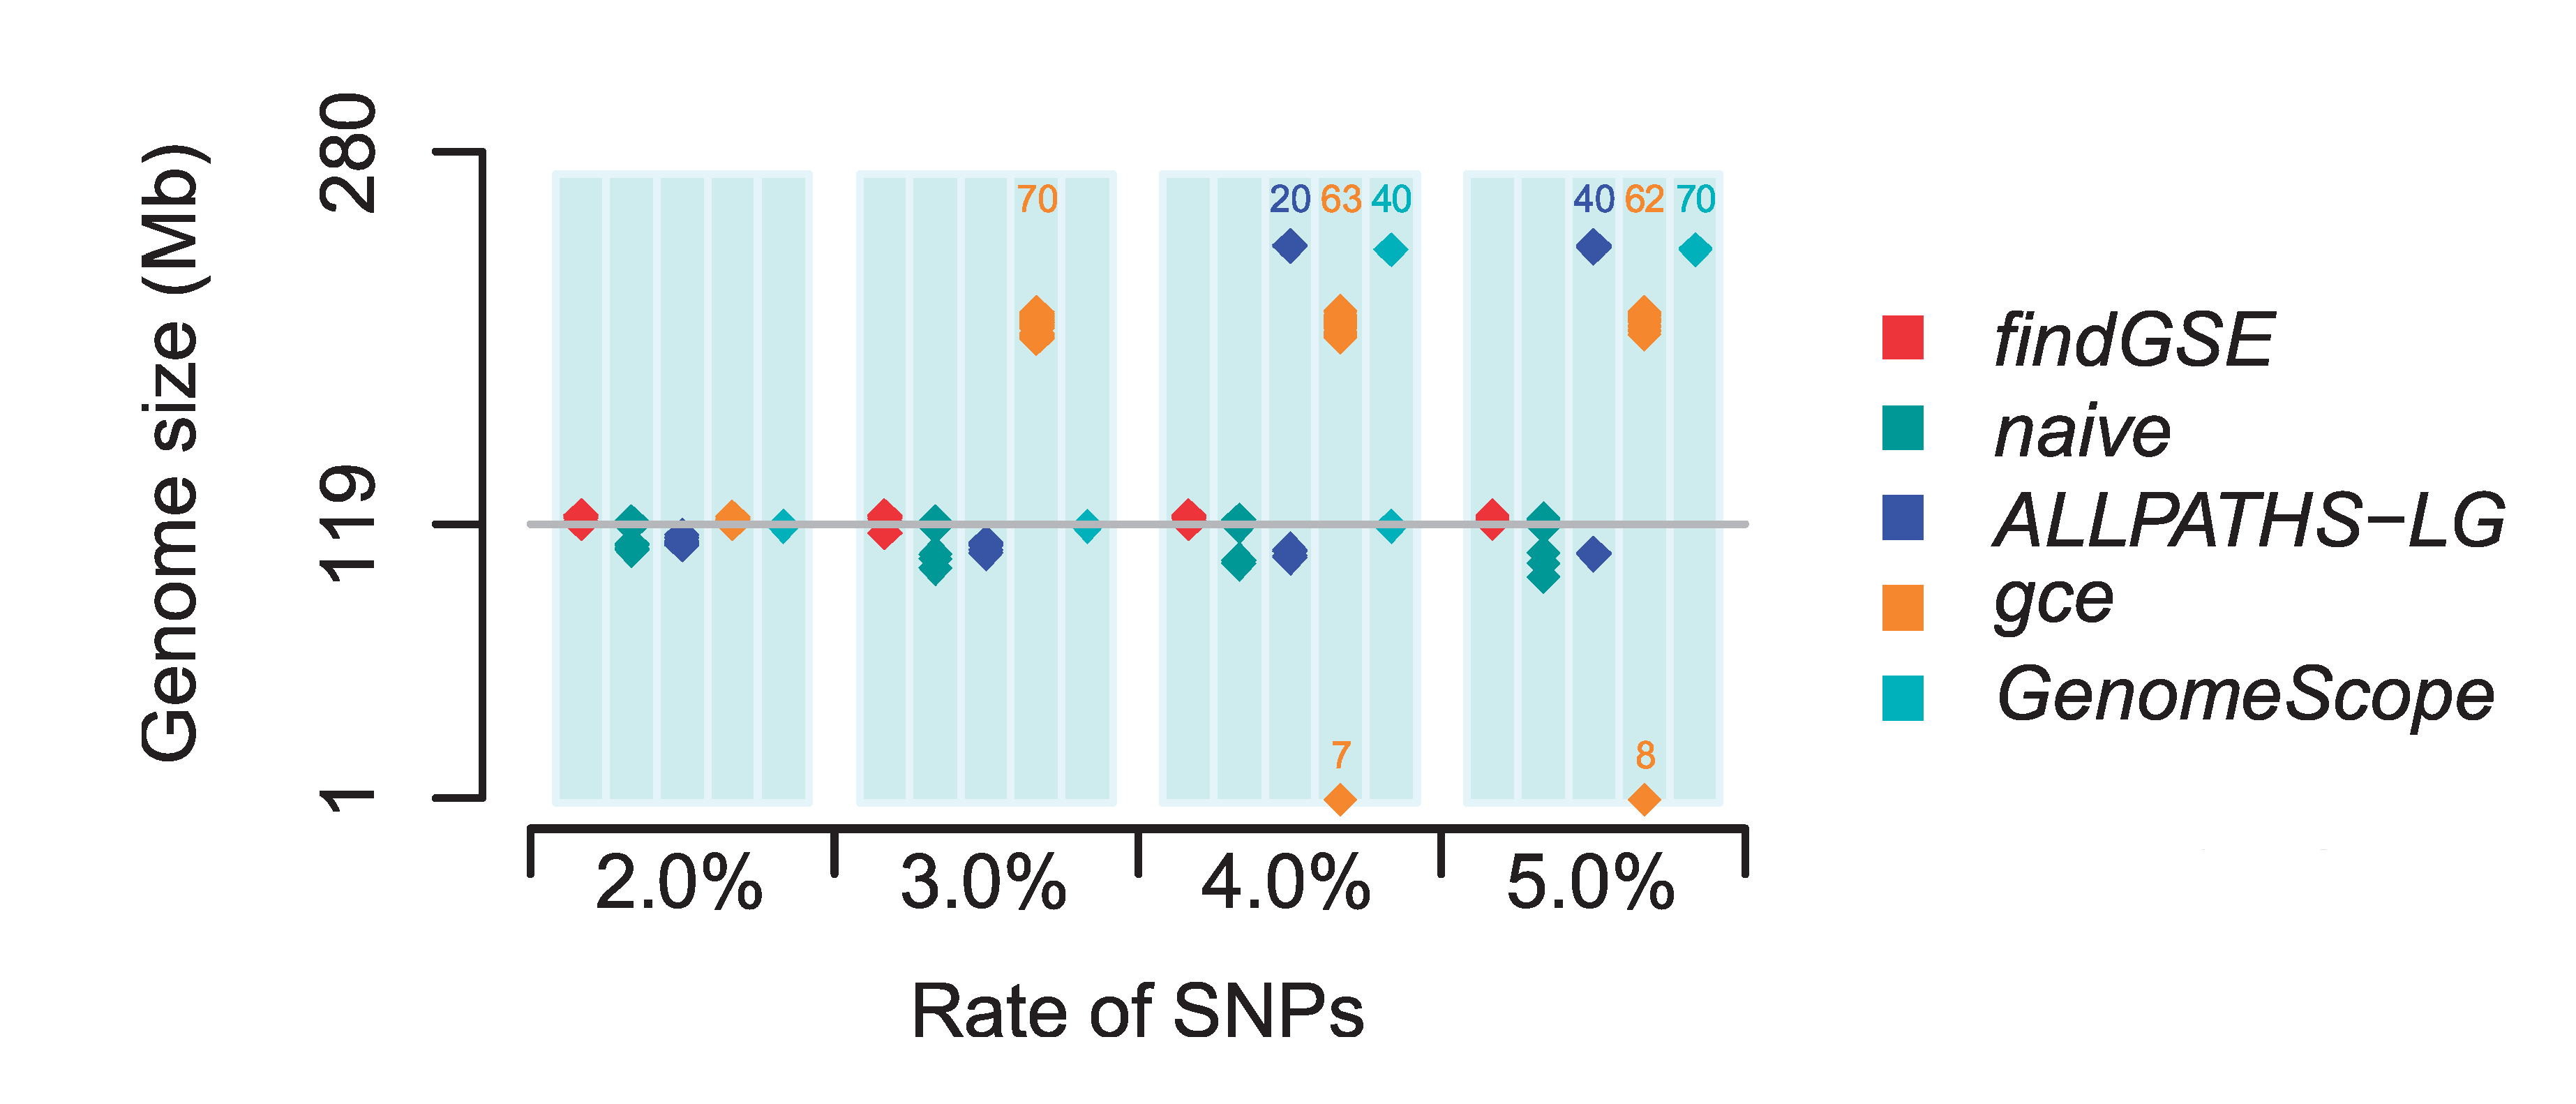
\includegraphics[height=0.21\textheight]{capitoli/analisi/confronto/confronto1/e.png}
	 	\caption{Stima della dimensione del genoma con livello di eterozigosi variabile e copertura base 100$\times$. Si noti che i valori rappresentati indicano il numero di punti sovrapposti in una certa regione.}
	 	\label{fig:confronto4}
	 \end{figure}
 
 	\paragraph{Stima di sequenze reali}
 	La riproducibilità dei metodi analizzati è stata verificata con la stima della dimensione di sette genomi reali. Le sequenze scelte per la verifica sono sequenziamenti di \textit{Arabidopsis thaliana}, le cui differenze si assume non vadano a modificare considerevolmente la dimensione del genoma. La deviazione standard delle stime per ciascun metodo si presenta bassa, variando tra 2 Mb (findGSE) e 5 Mb (GCE), come mostra la figura~\vref{fig:confronto5a}. Ciò può dimostrare la robustezza dei programmi rispetto ad eventuali variazioni nel sequenziamento del genoma, e l'alta riproducibilità che li caratterizza.

 	Per verificare l'indipendenza tra il valore stimato e la copertura di letture reali, i metodi sono stati utilizzati per stimare la dimensione del genoma di \textit{A. thaliana} a partire da 89 sequenze con copertura base minima maggiore di 19$\times$. Come mostra la figura~\vref{fig:confronto5b}, le stime di ciascun programma risultano indipendenti da tale valore.
 	
 	\begin{figure}[p]
 		\centering
 		\subfloat[][\emph{Valori stimati, media e deviazione standard di ciascun metodo.}\label{fig:confronto5a}]
 			{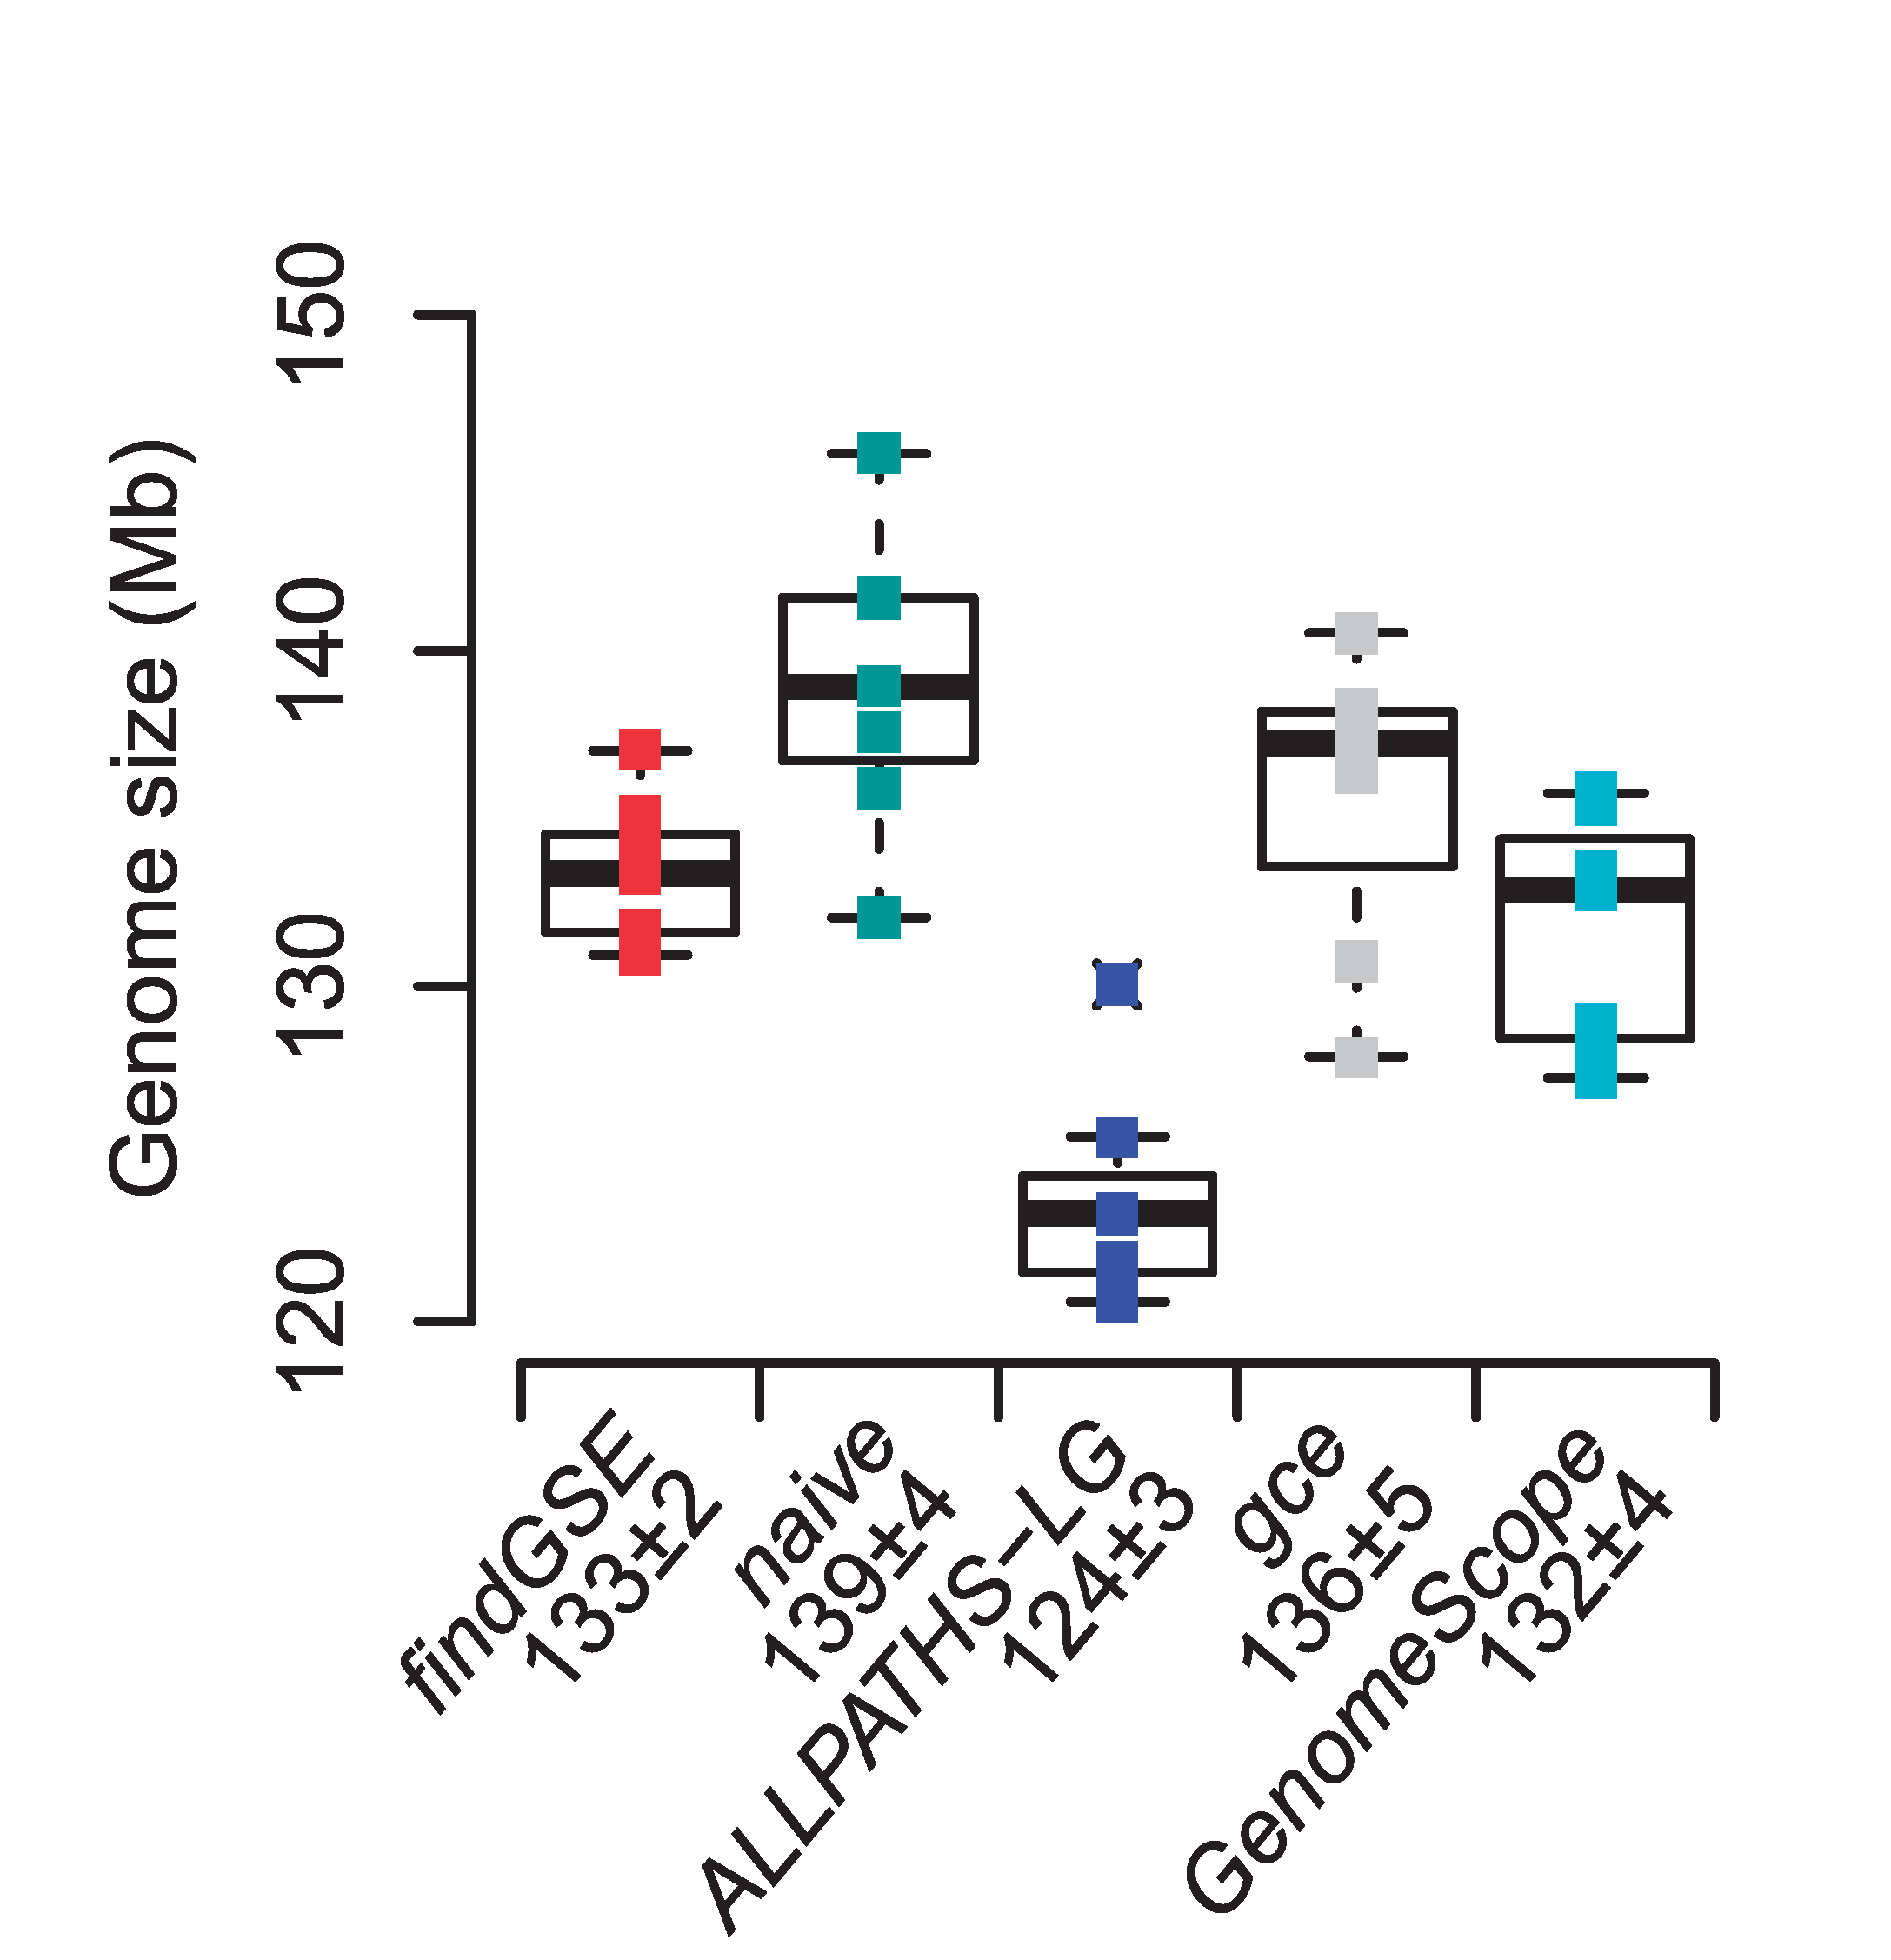
\includegraphics[width=0.37\textwidth]{capitoli/analisi/confronto/confronto1/f.png}} \qquad 
 		\subfloat[][\emph{Valori stimati da ciascun metodo in relazione alla copertura base.}\label{fig:confronto5b}]
 			{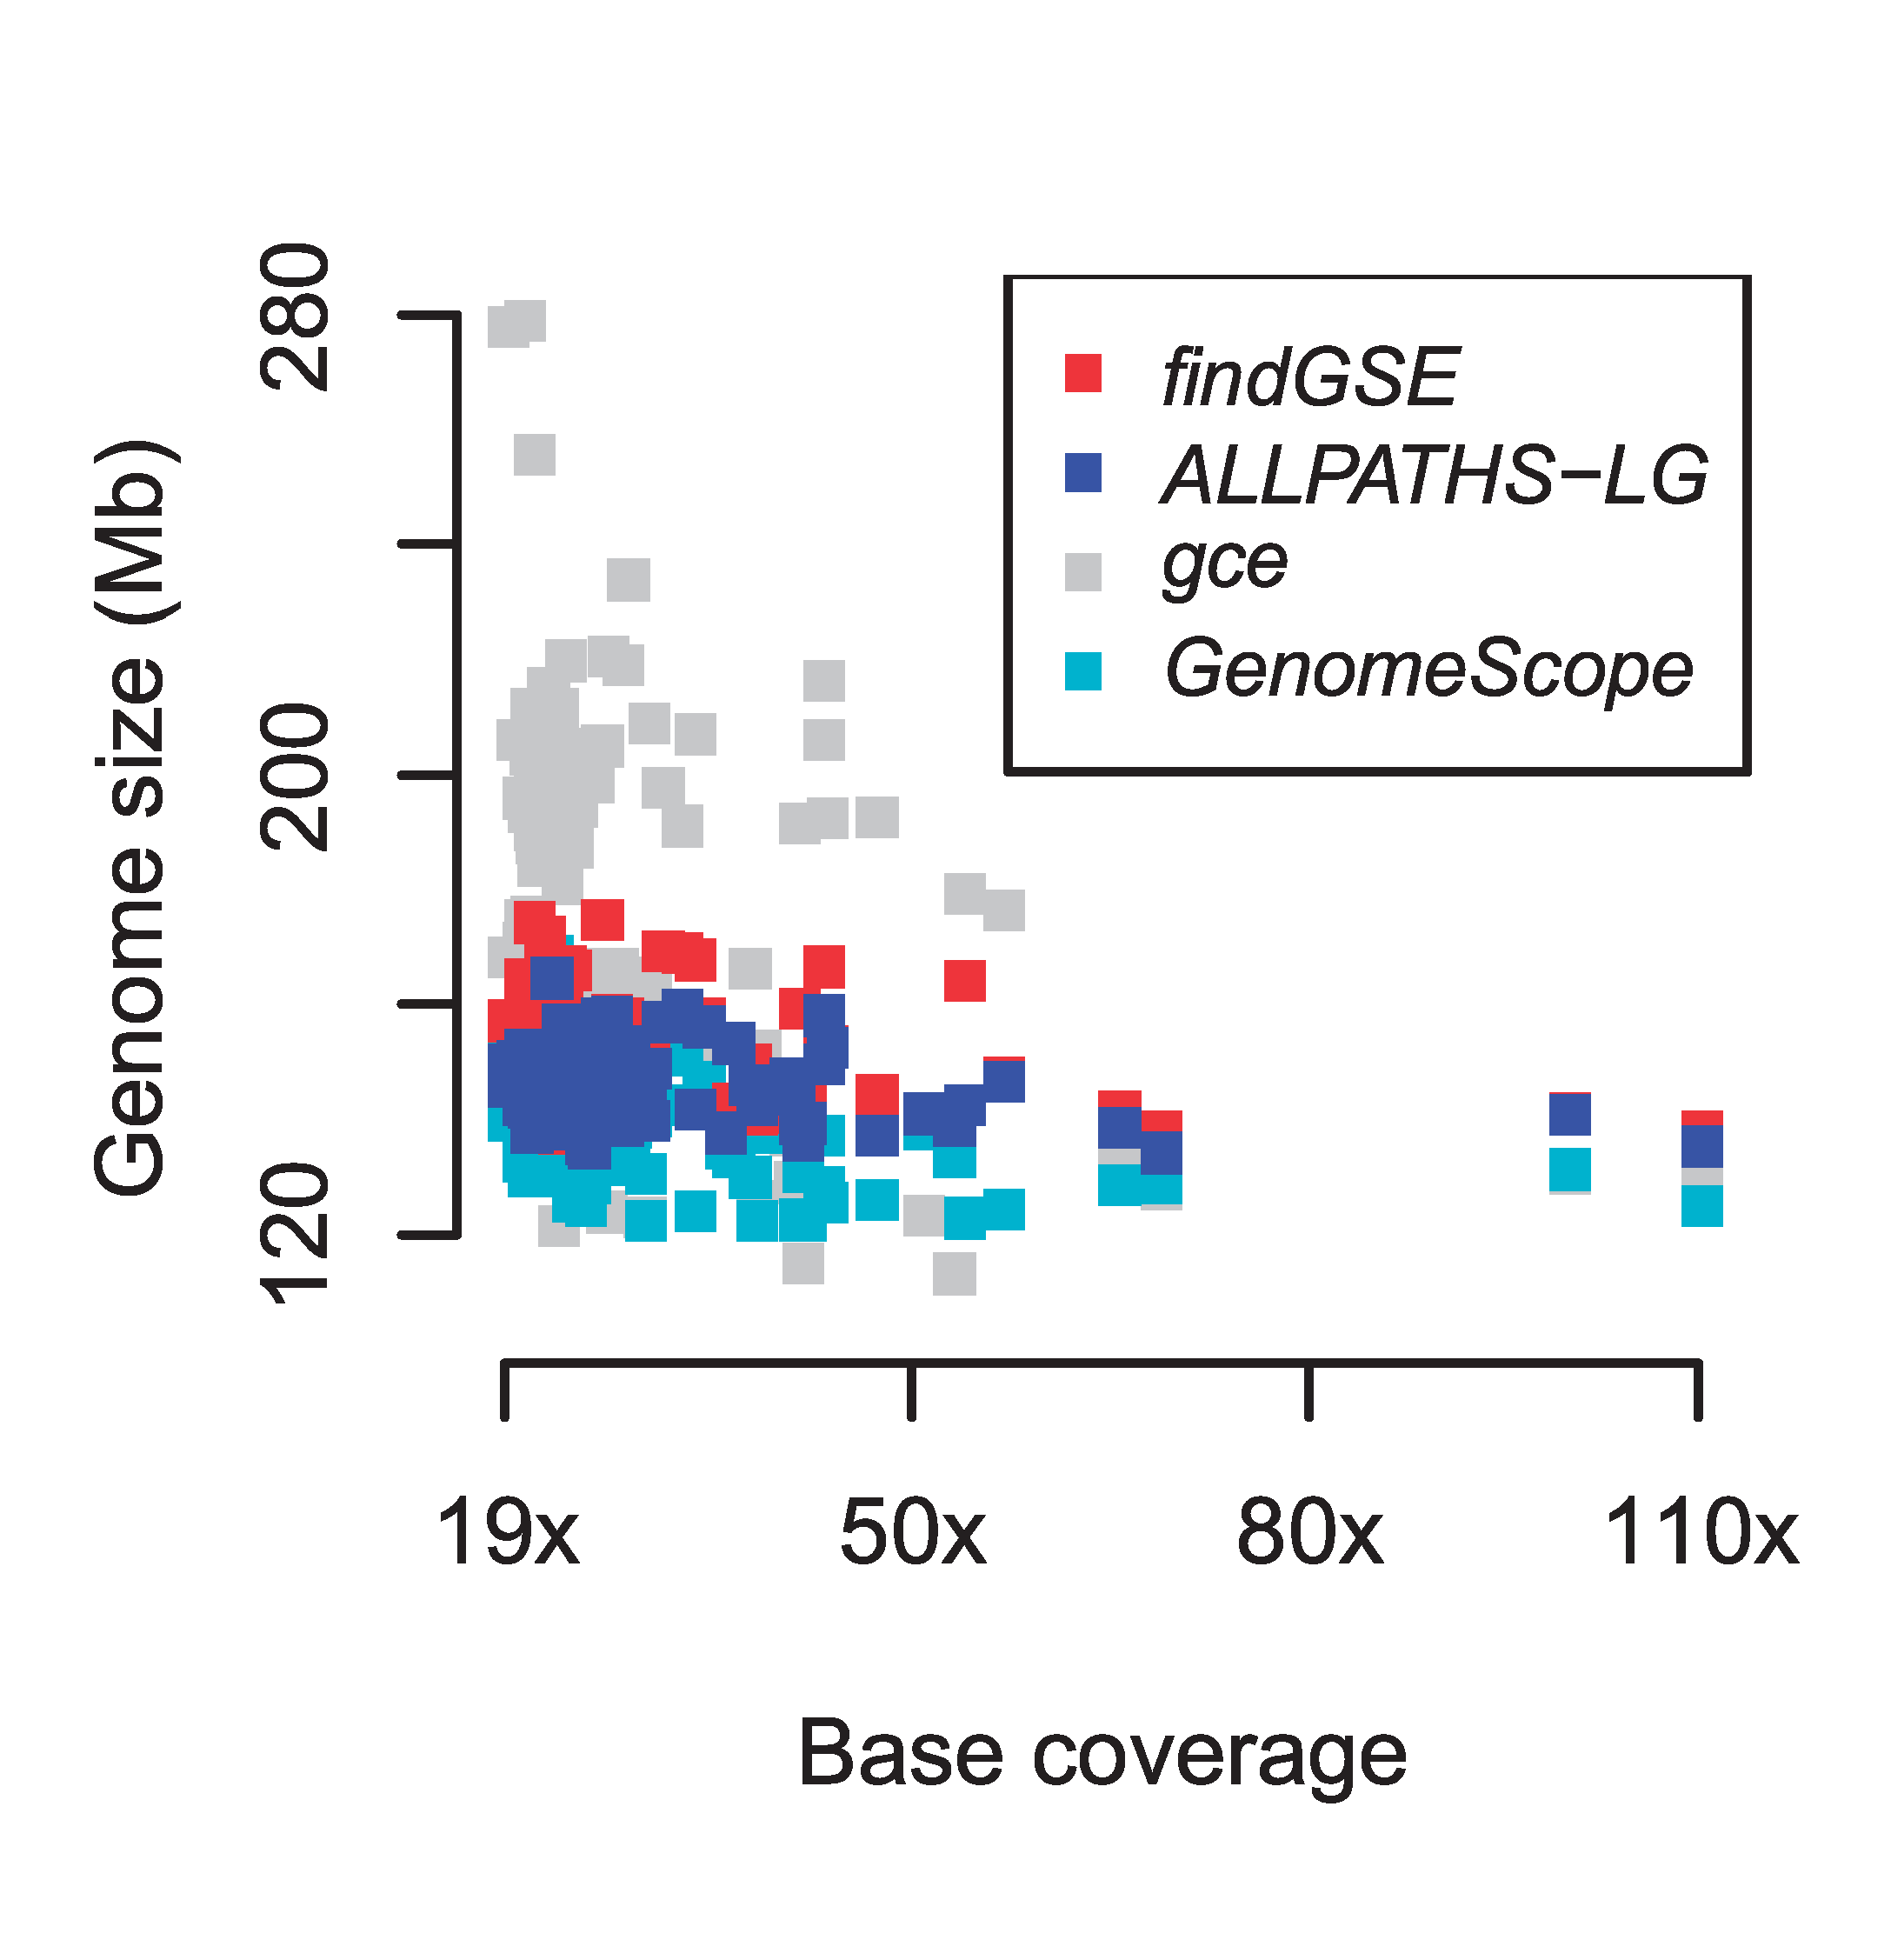
\includegraphics[width=0.37\textwidth]{capitoli/analisi/confronto/confronto1/g.png}} 
 		\caption{Confronto tra i metodi analizzati nella stima della dimensione di \textit{A. thaliana}.}
 		\label{fig:confronto5}
 	\end{figure}
 
	\paragraph{Confronto con flow cytometry}
	Sebbene il metodo flow cytometry non possa restituire una dimensione certa del genoma, è considerato un metodo sperimentale che la possa almeno approssimare. Analizzando la dimensione di 89 sequenze di \textit{A. thaliana}, la deviazione standard della stima fatta dai programmi varia tra 6 Mb e 9 Mb. Il metodo flow cytometry invece mostra una deviazione standard di 4 Mb, che suggerisce una maggior stabilità della predizione. Per ciascun programma è stato quindi misurato il \gls{pcc} con il metodo flow cytometry (figura~\vref{fig:confronto6}), assumendo che un coefficiente più alto indichi una maggior capacità di rilevare variazioni reali della dimensione del genoma. La correlazione tra findGSE e il suddetto metodo risulta la più alta ($r = $ 0,524). 
	
	I metodi findGSE, ALLPATHS-LG e GenomeScope stimano in media simili valori di dimensione (rispettivamente 152, 146 e 138 Mb), mentre GCE produce un risultato inspiegabilmente grande (177 Mb). Il valore medio stimato tramite flow cytometry invece è di 167 Mb, anche se tale metodo tende a sovrastimarne la dimensione.
	\begin{figure}[p]
		\centering
		\subfloat[][\emph{Correlazione tra i valori stimati da GCE e flow cytometry.}\label{fig:confronto6a}]
			{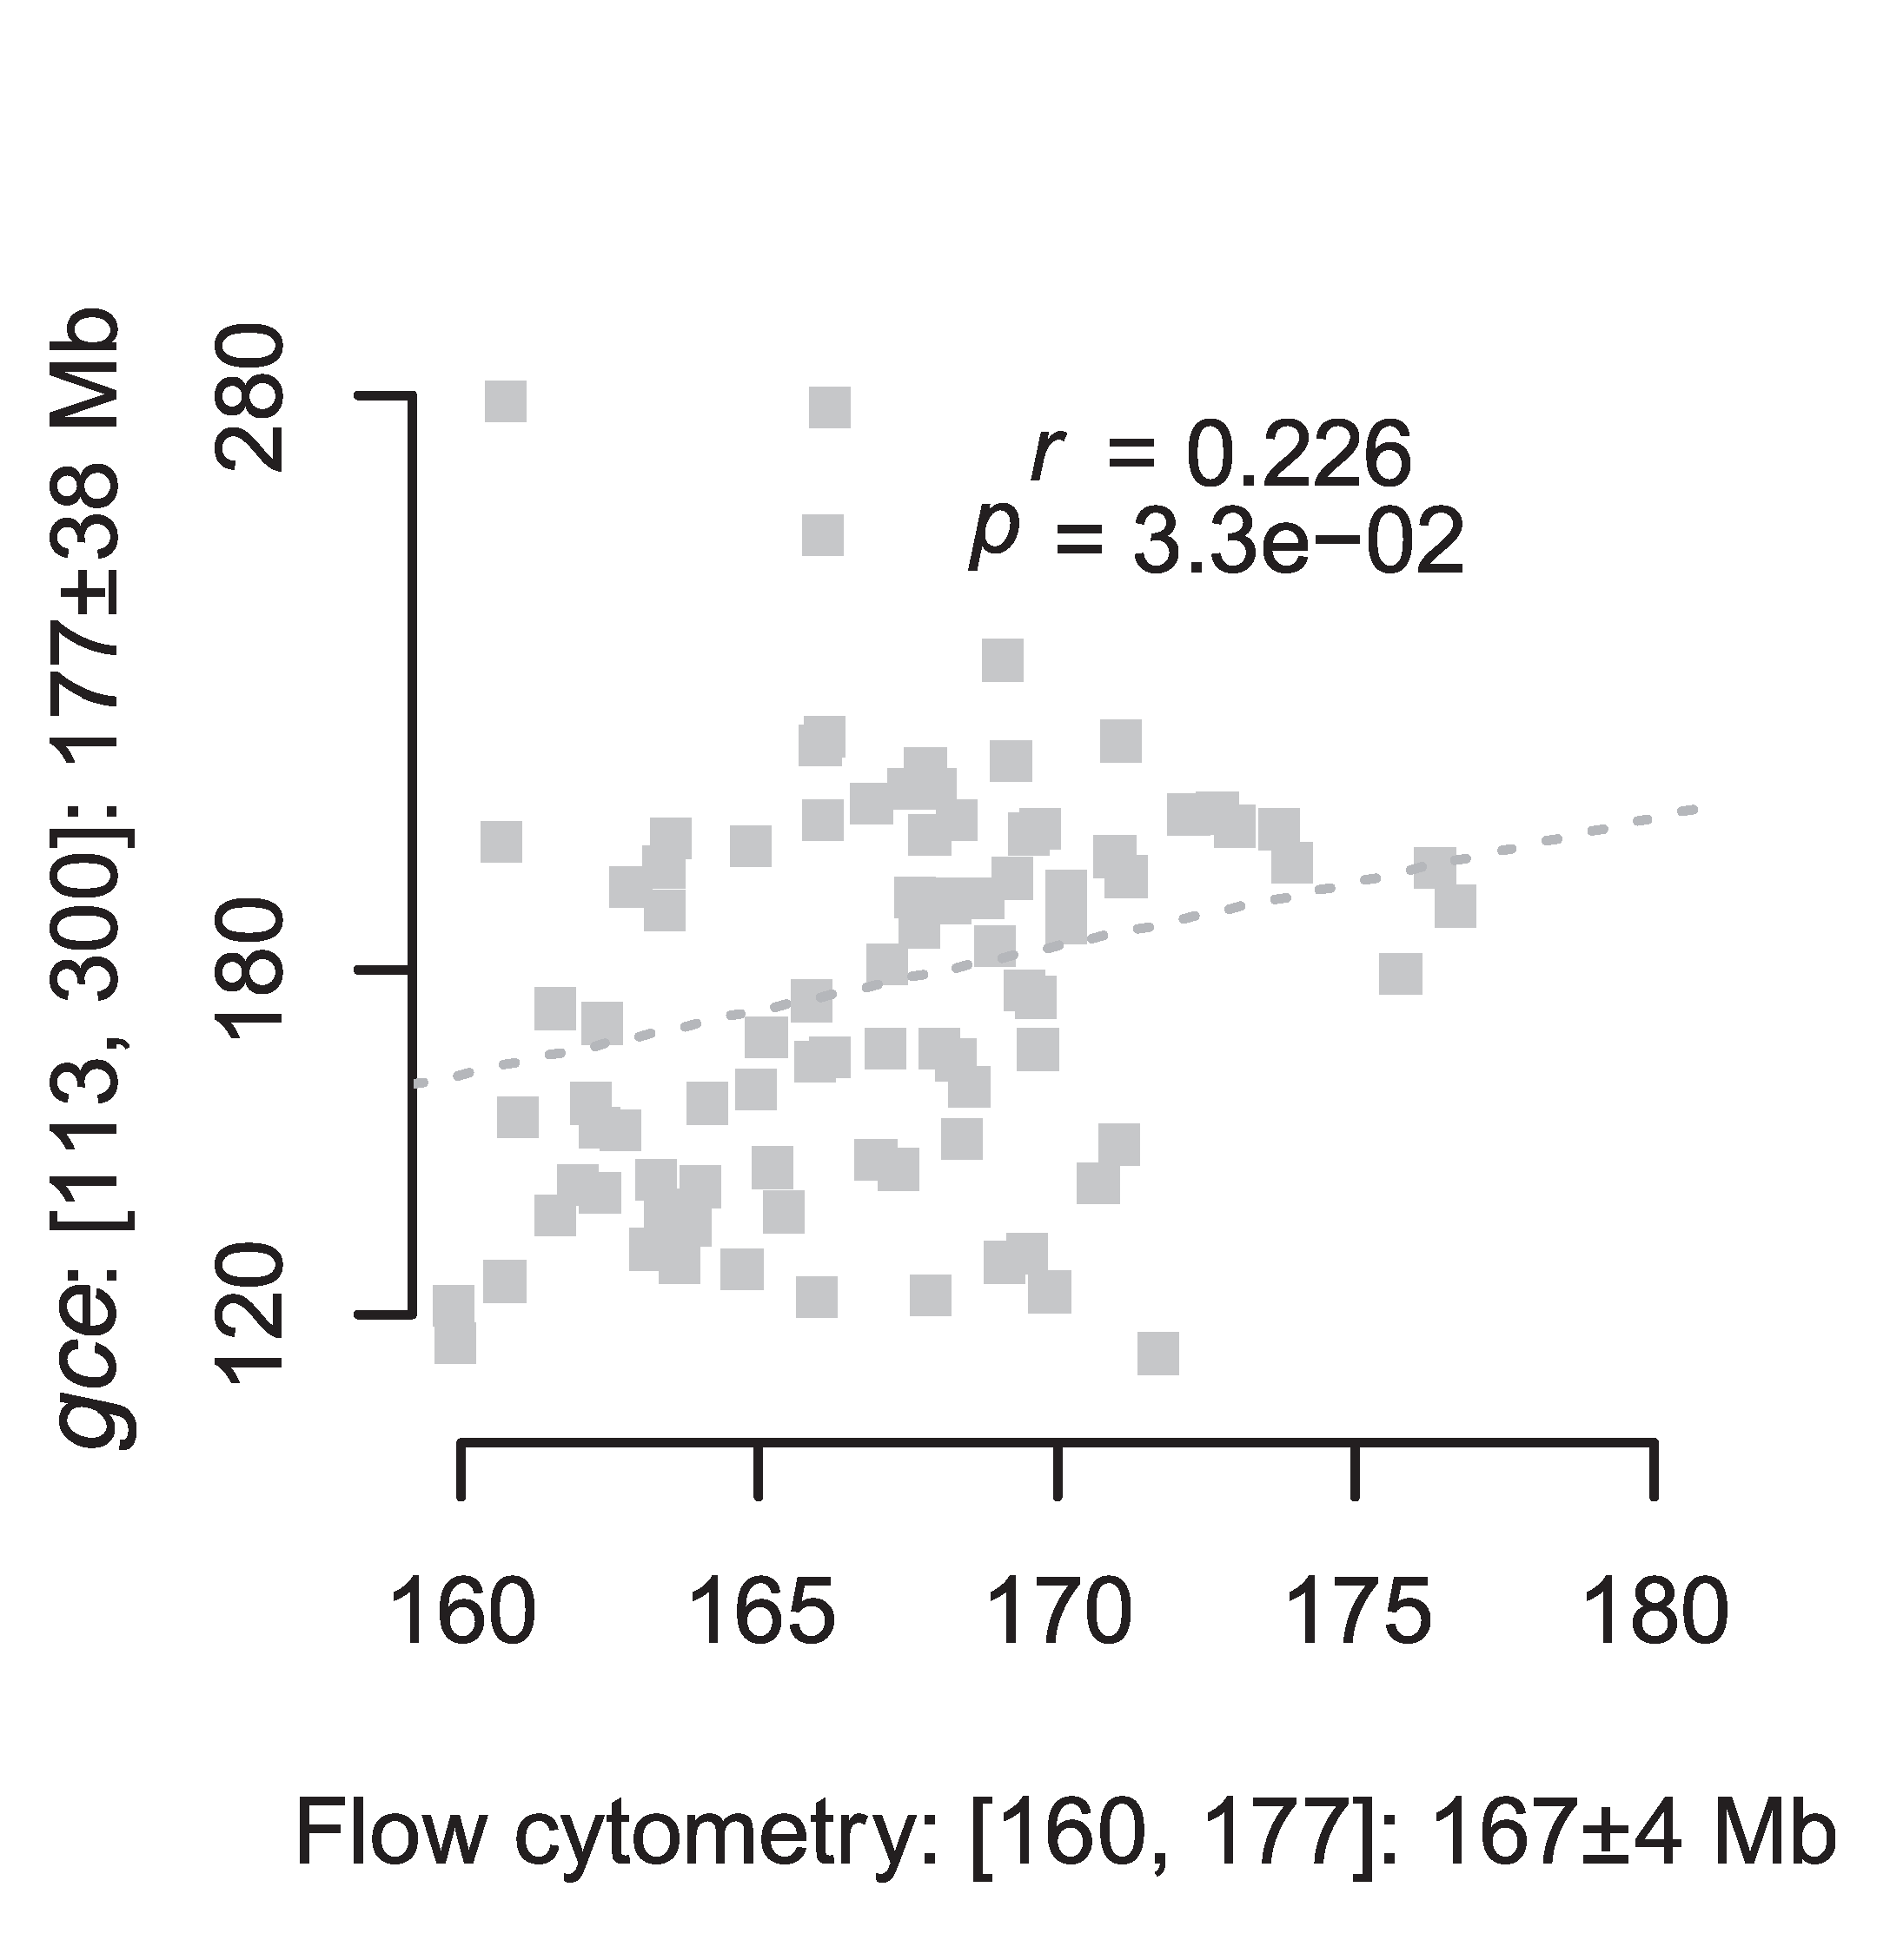
\includegraphics[width=0.37\textwidth]{capitoli/analisi/confronto/confronto1/h.png}} \qquad 
		\subfloat[][\emph{Correlazione tra i valori stimati da GenomeScope e flow cytometry.}\label{fig:confronto6b}]
			{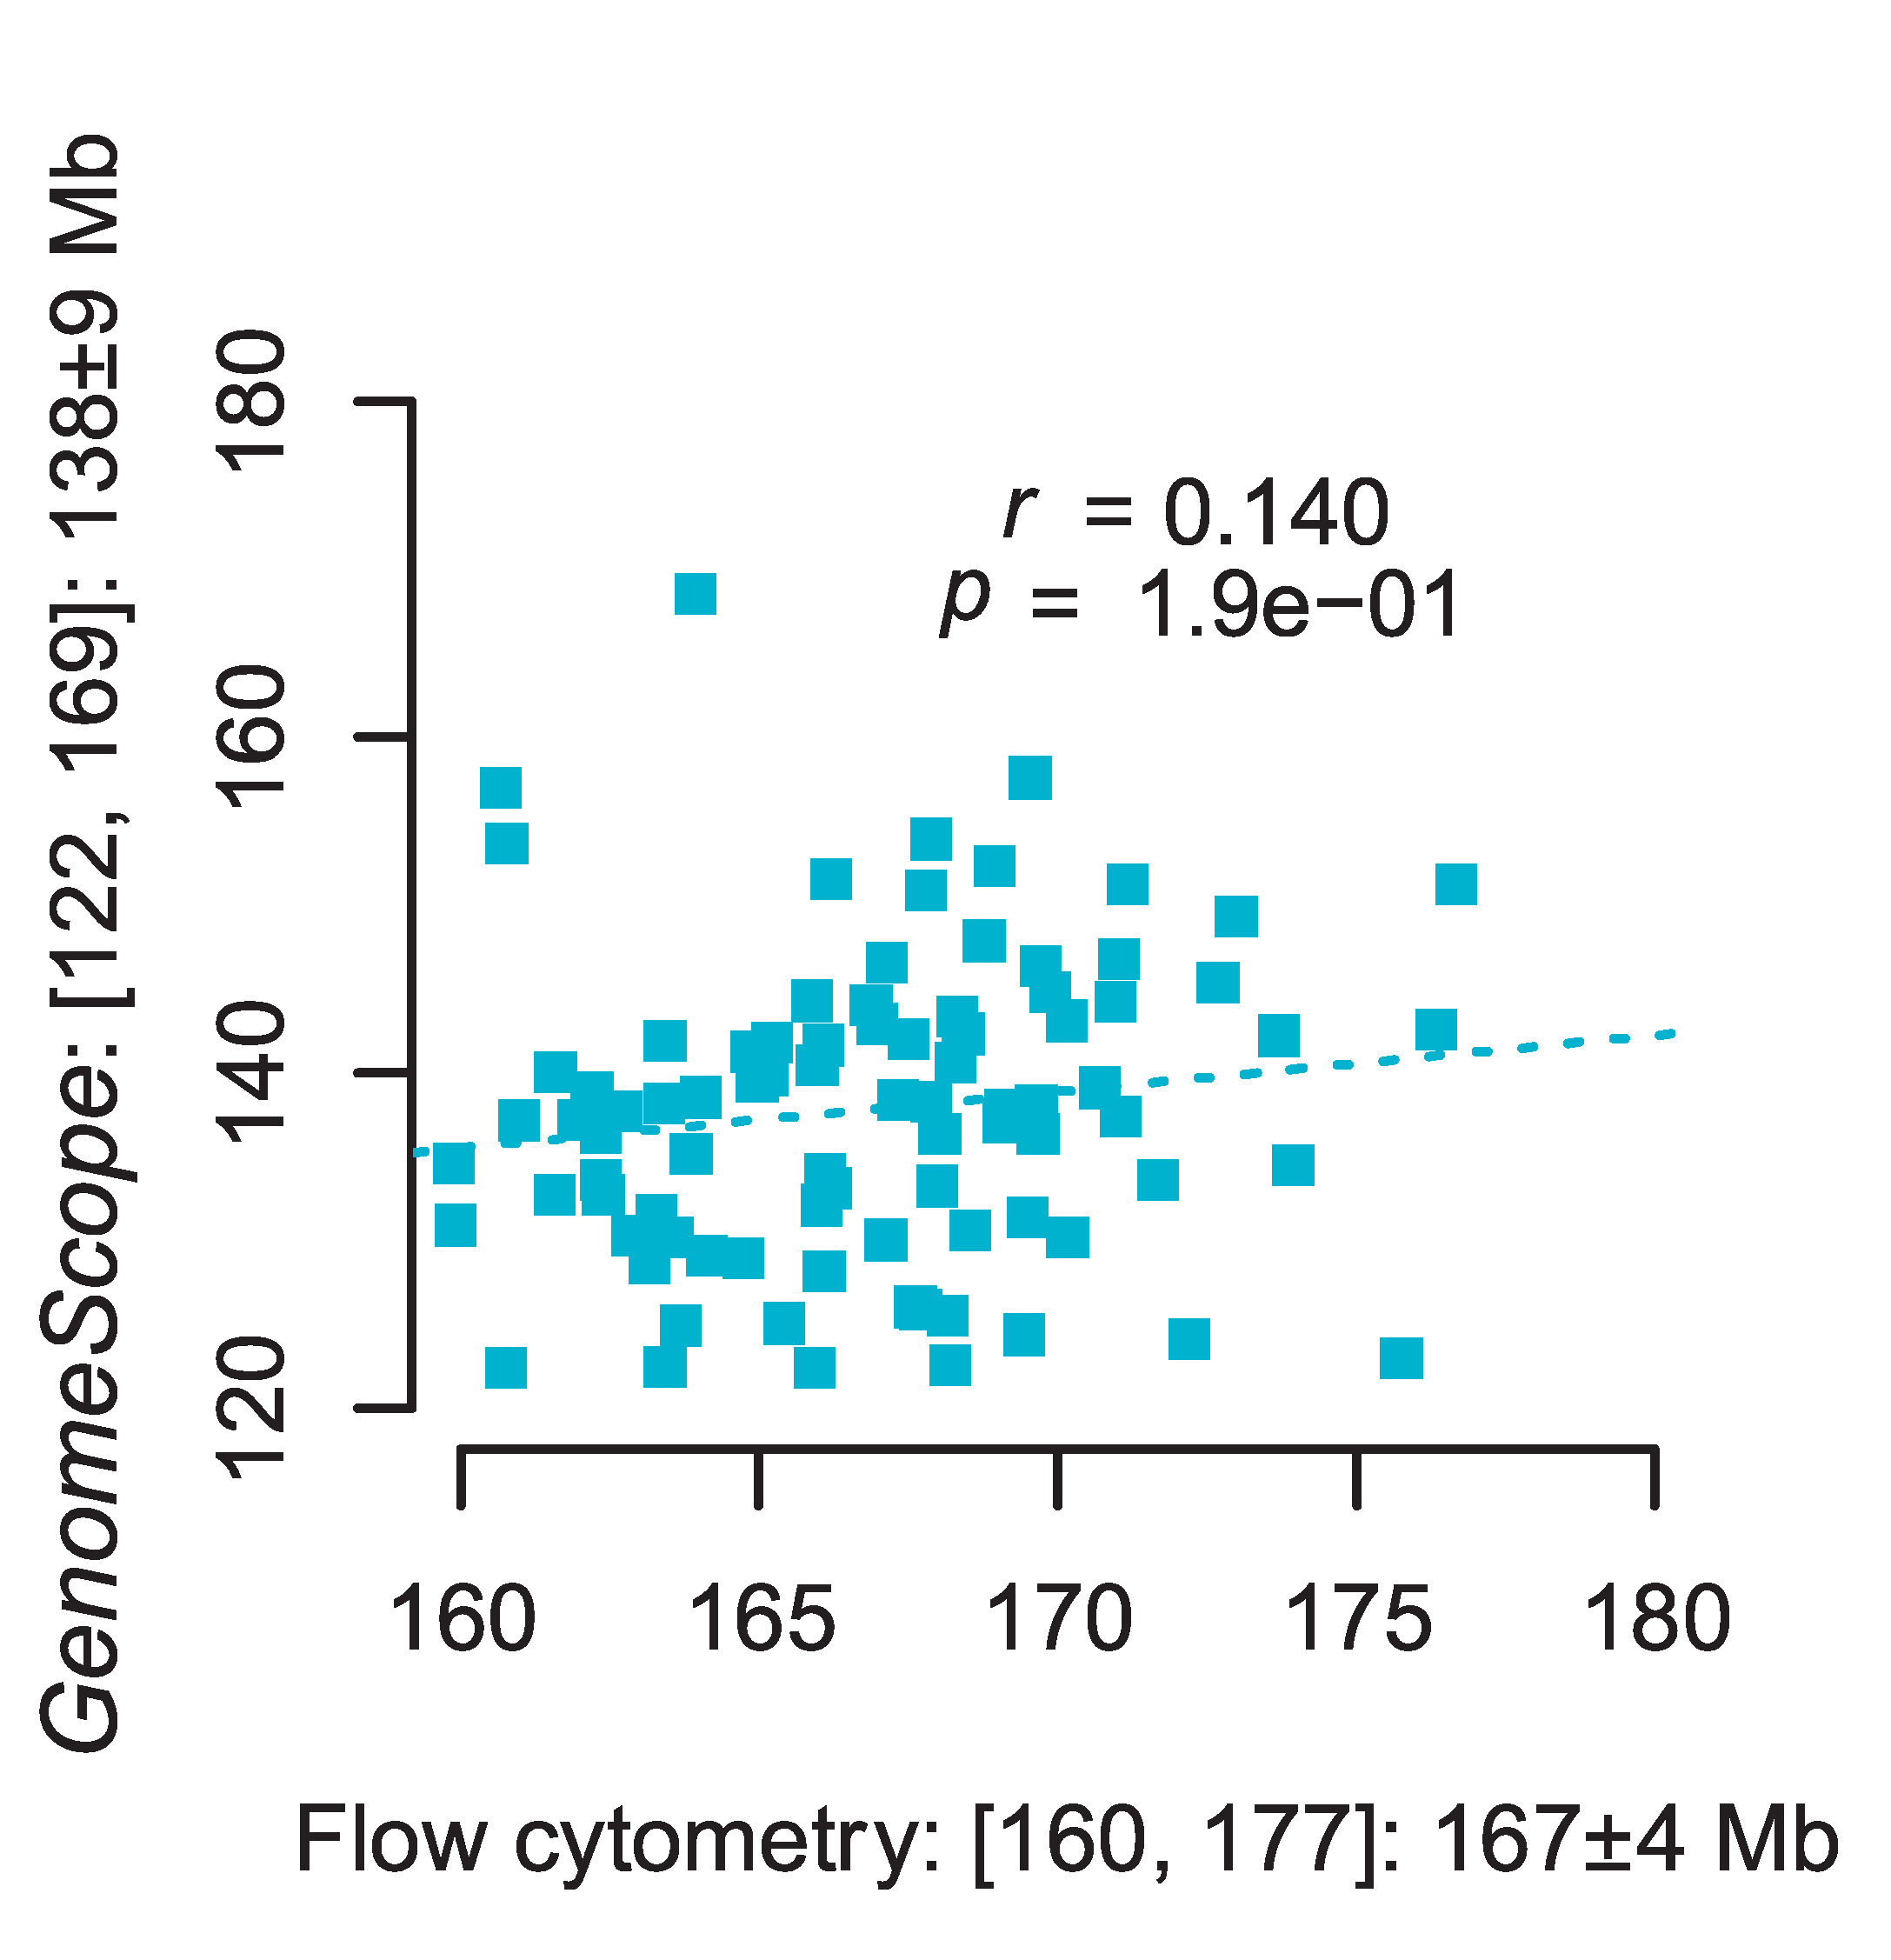
\includegraphics[width=0.37\textwidth]{capitoli/analisi/confronto/confronto1/i.png}} \\
		\subfloat[][\emph{Correlazione tra i valori stimati da ALLPATHS-LG e flow cytometry.}\label{fig:confronto6c}]
			{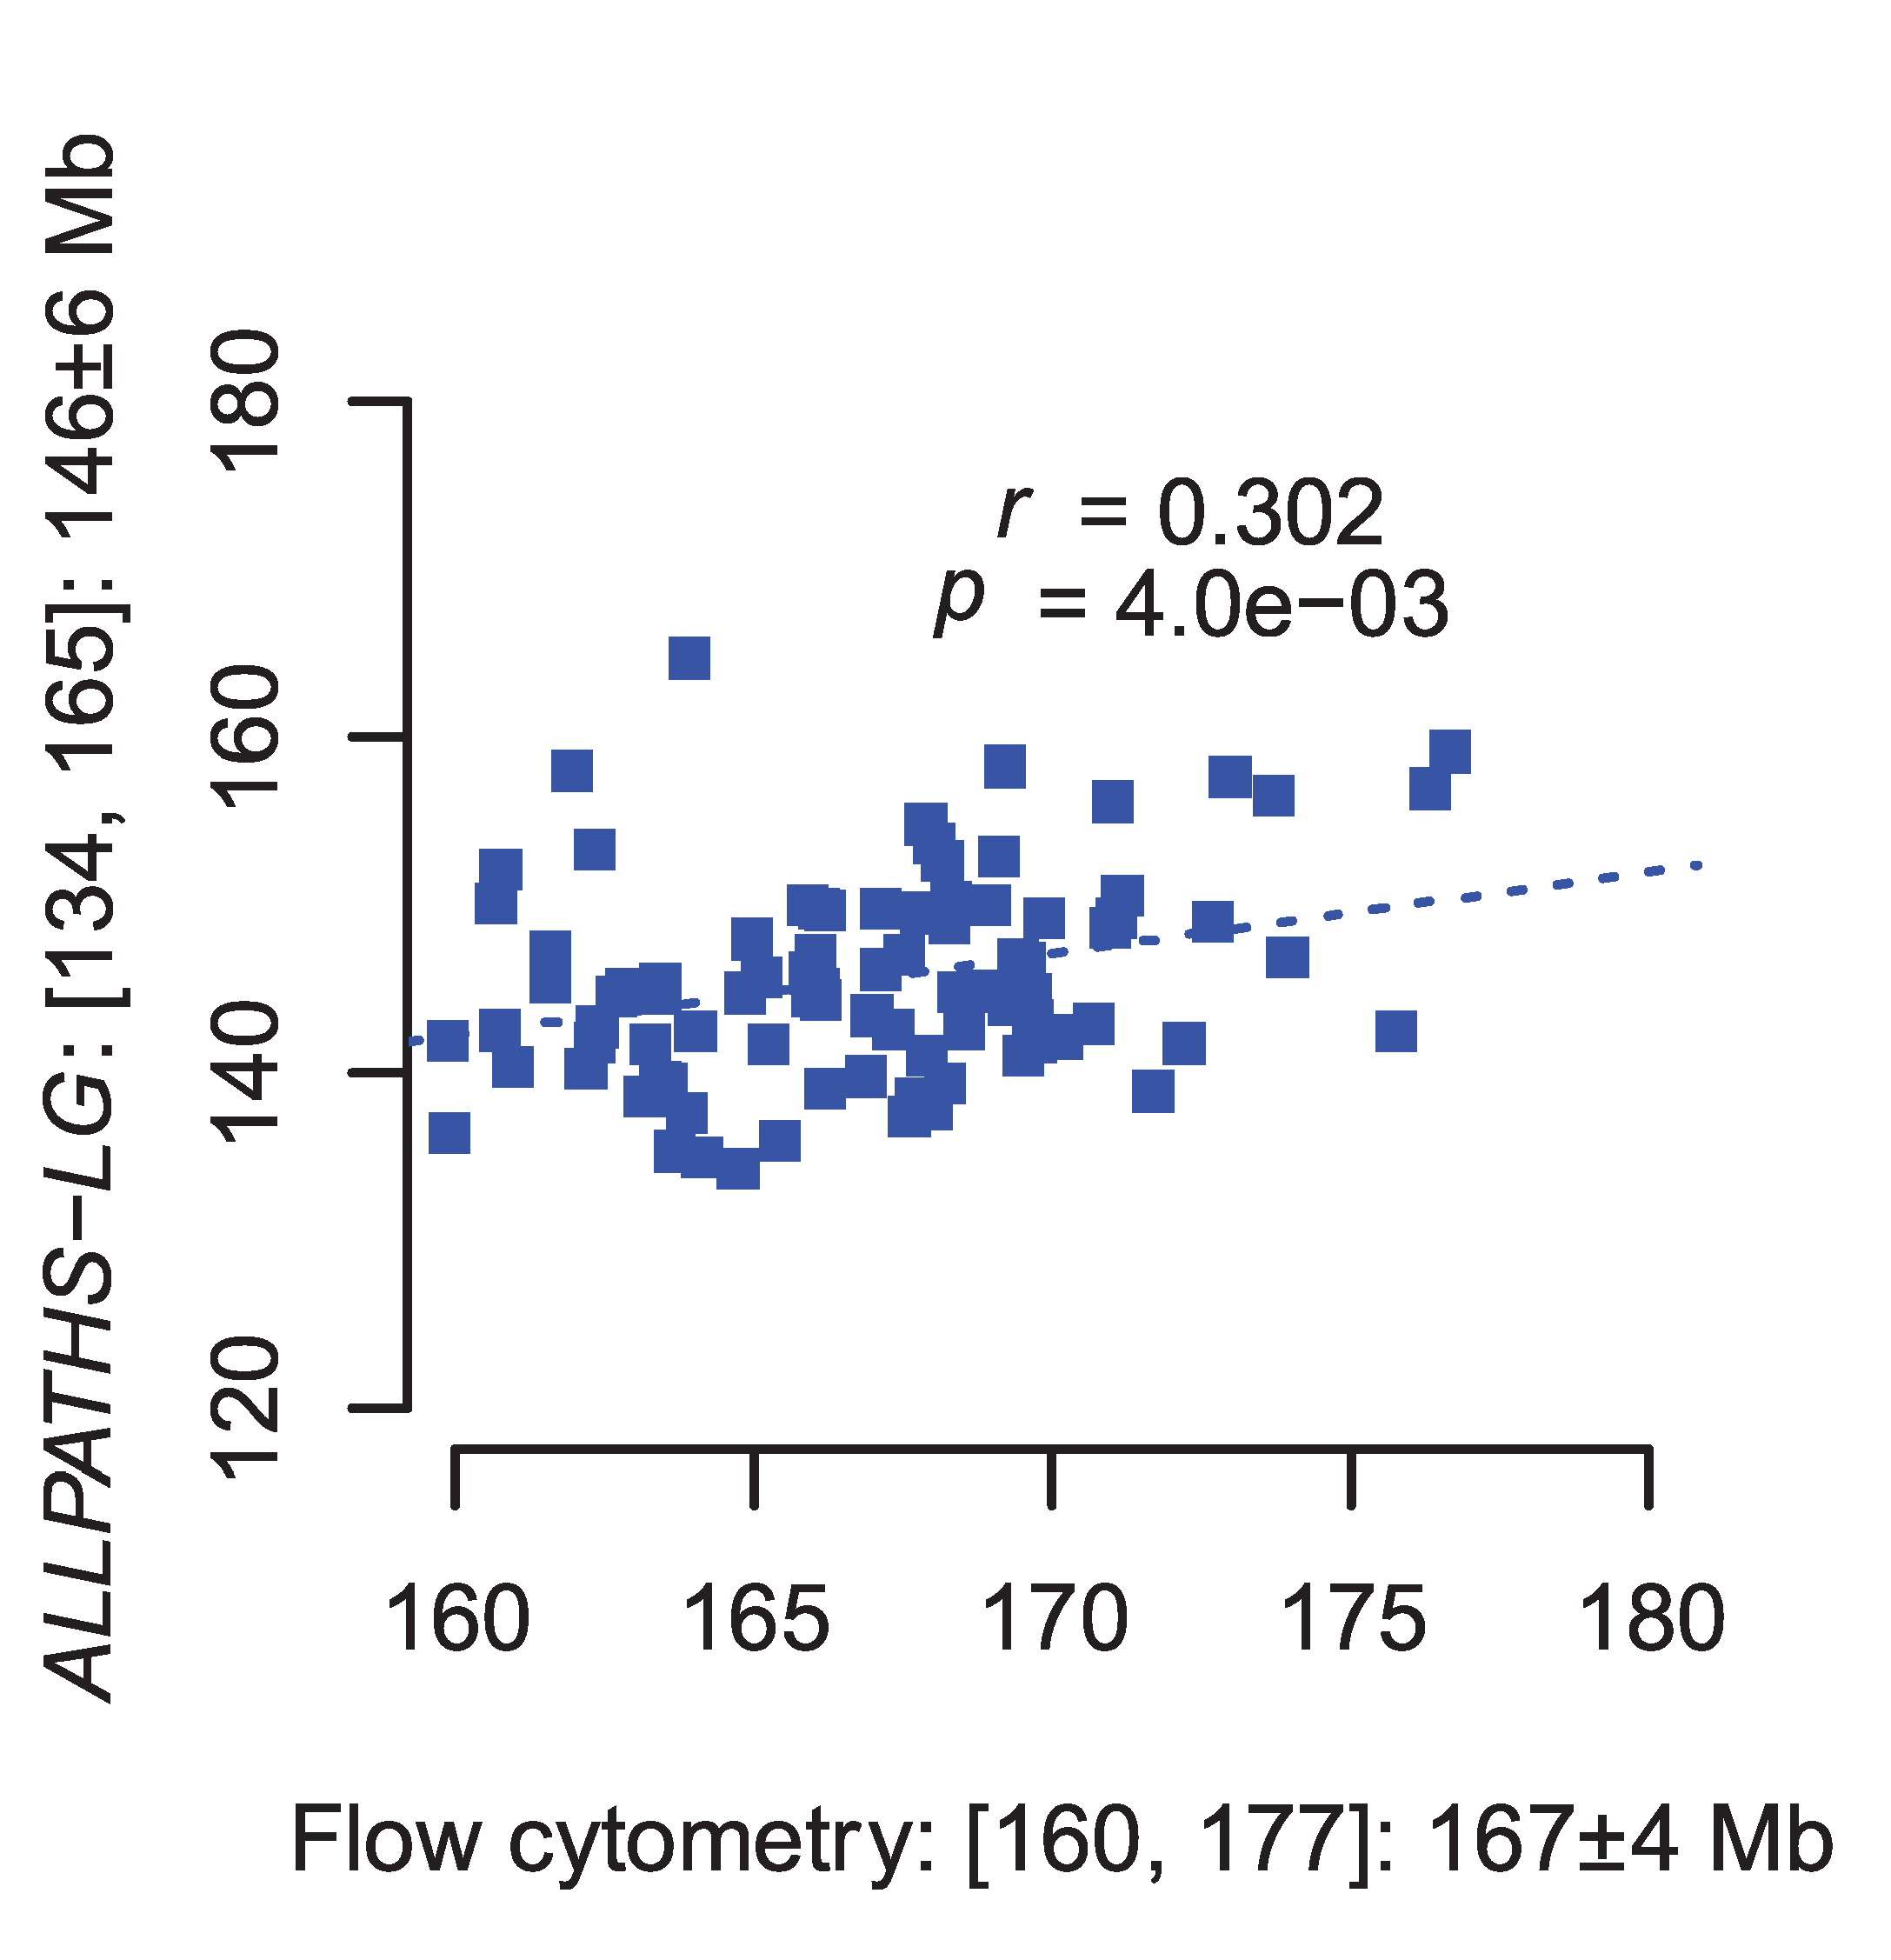
\includegraphics[width=0.37\textwidth]{capitoli/analisi/confronto/confronto1/l.png}} \qquad 
		\subfloat[][\emph{Correlazione tra i valori stimati da findGSE e flow cytometry.}\label{fig:confronto6d}]
			{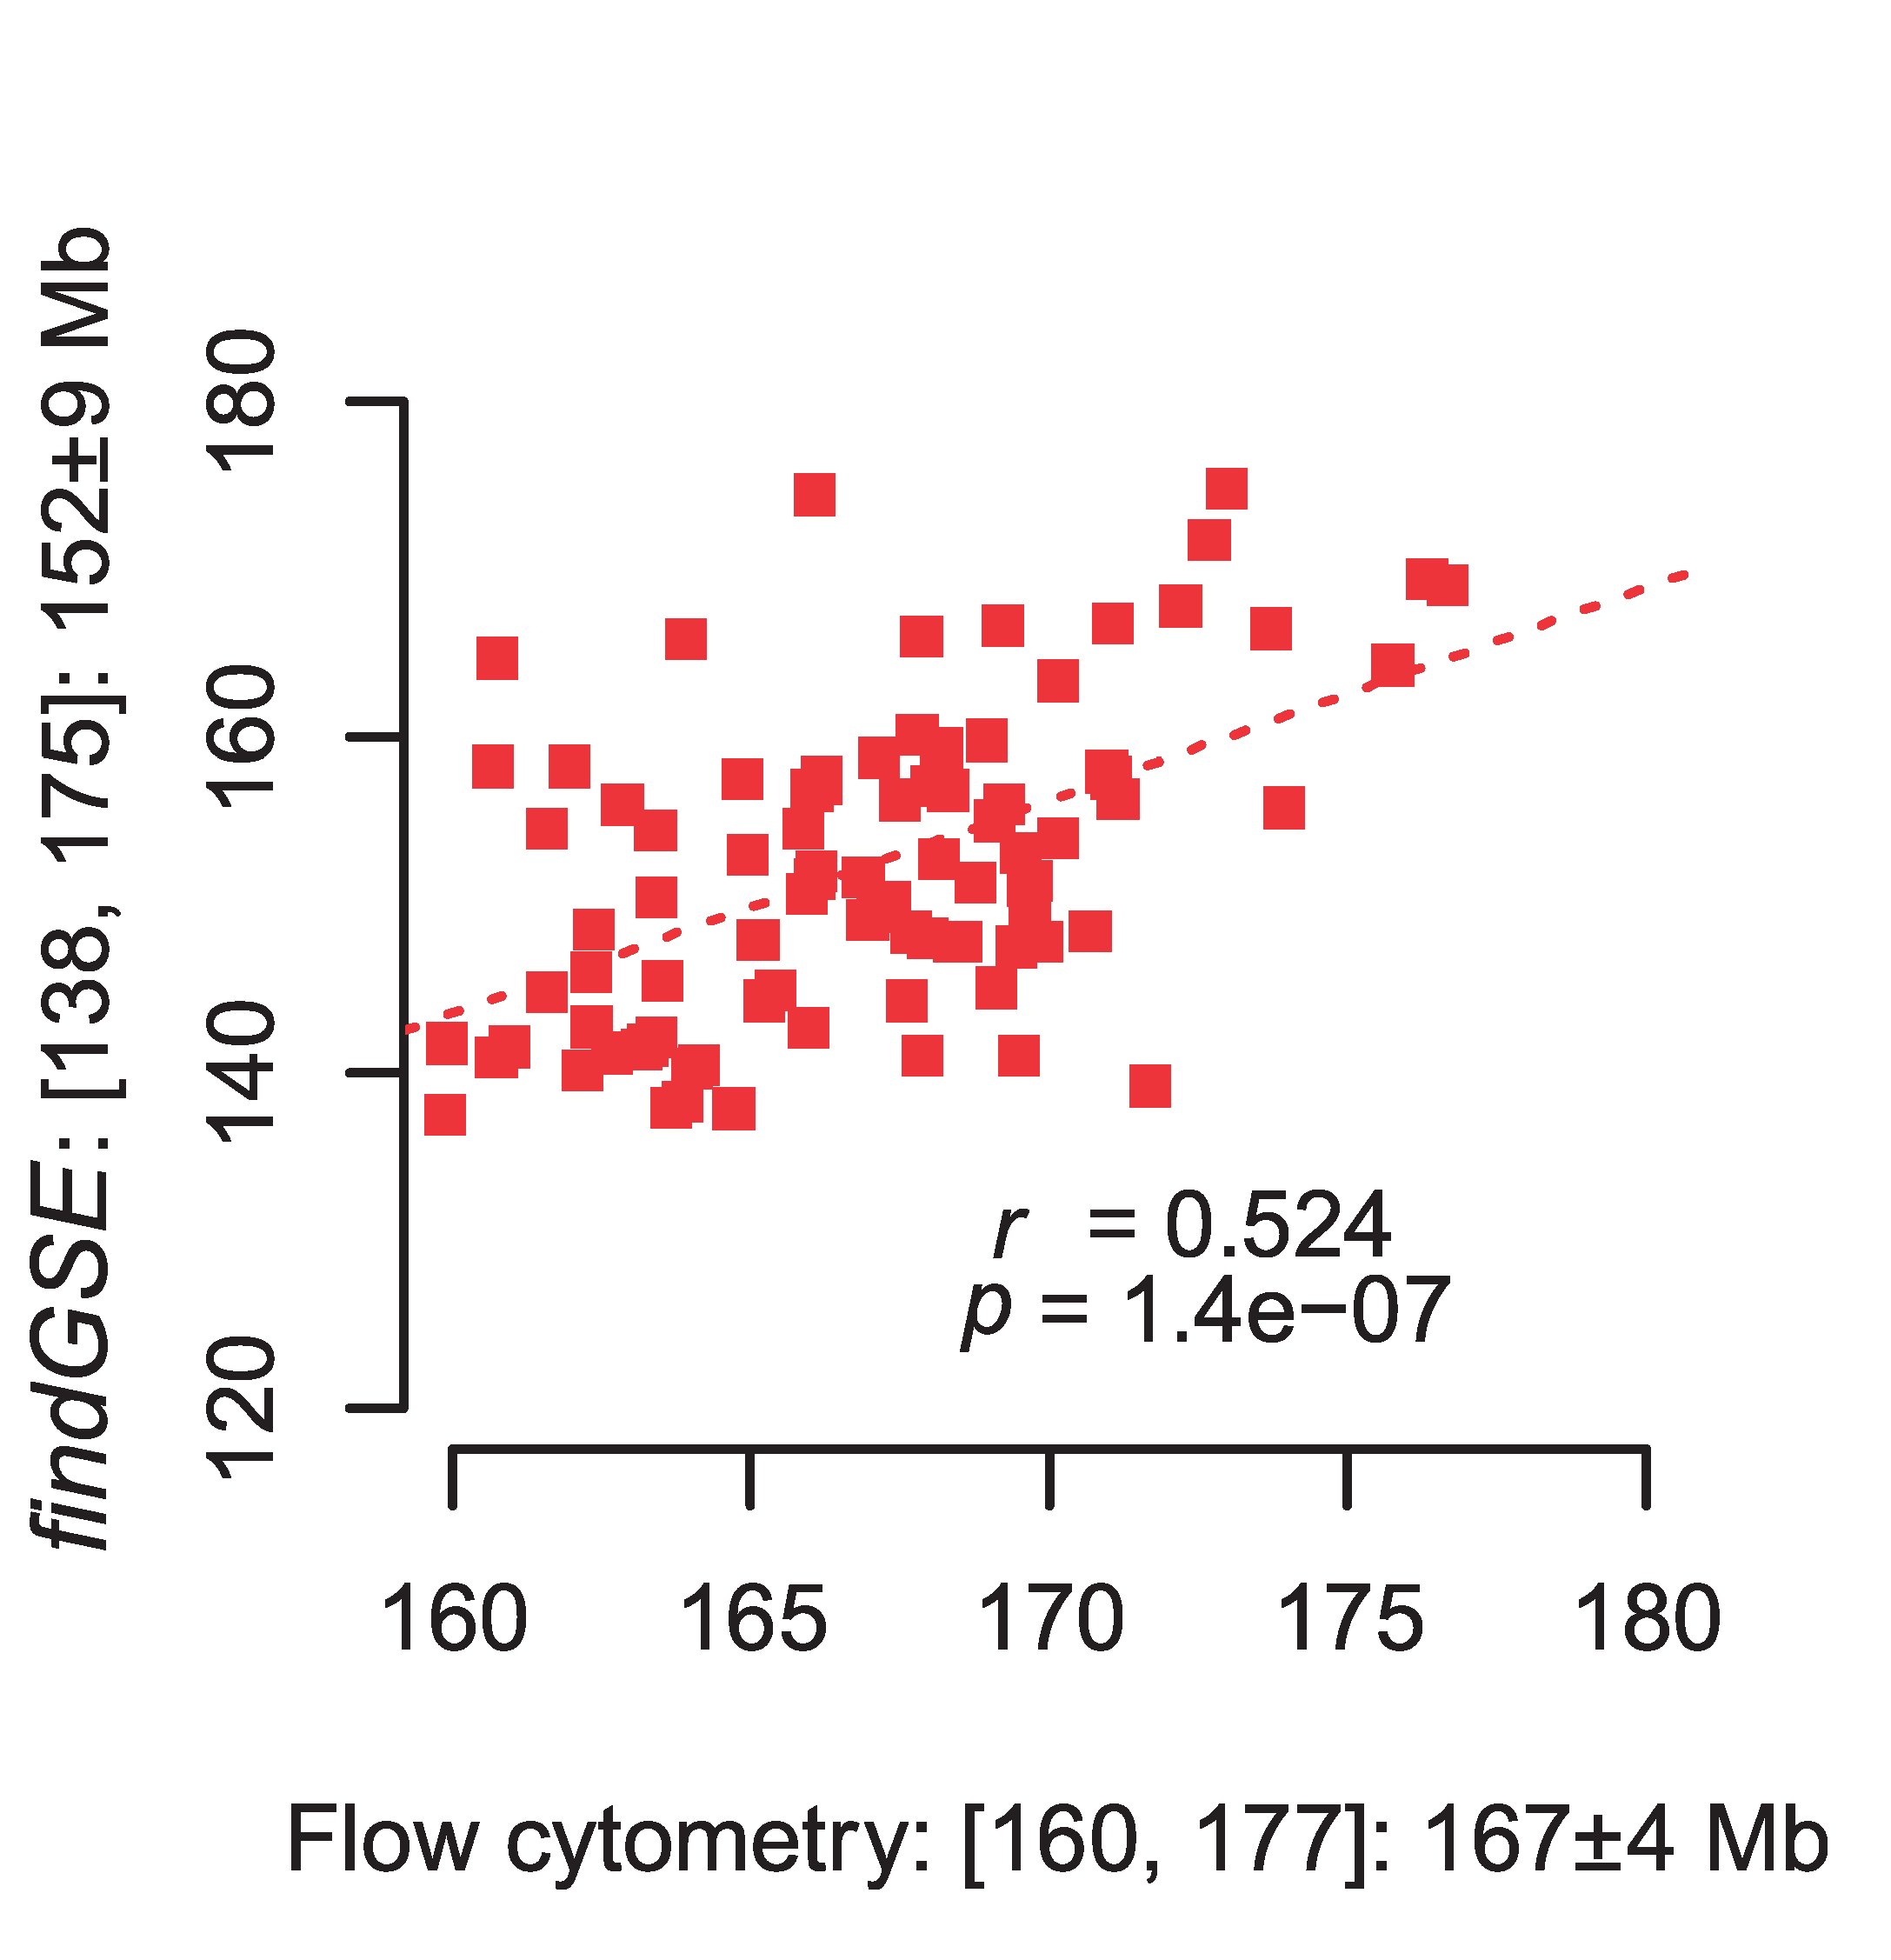
\includegraphics[width=0.37\textwidth]{capitoli/analisi/confronto/confronto1/m.png}} 
		\caption{Correlazione tra i metodi analizzati e flow cytometry. In ciascuna figura sono raffigurate anche la regressione lineare e il \gls{pcc} $r$.}
		\label{fig:confronto6}
	\end{figure}

\end{document}
	\documentclass[crop=false, class=book]{standalone}

\begin{document}
		
	\subsection{Metodi MGSE, GenomeScope, GCE e findGSE}
	I dati e le figure della seguente analisi sono state ricavate da \cite{pucker2019MGSE}, che esegue un confronto tra i metodi MGSE, GenomeScope, GCE e findGSE. 
	
	Dopo una comparazione iniziale processando due diversi ecotipi di \textit{Arabidopsis thaliana}, i programmi vengono utilizzati per la stima della dimensione di genomi con grandezze e complessità maggiori, come le specie \textit{Beta vulgaris}, \textit{Brachypodium distachyon}, \textit{Solanum lycopersicum}, \textit{Zea mays} e \textit{Vitis vinifera}. 
		
	\paragraph{Stima della dimensione di \textit{A. thaliana}}
	Inizialmente i programmi in esame vengono utilizzati per il calcolo della dimensione delle varianti Col-0 e Nd-1 di \textit{Arabidopsis thaliana}. Per i metodi GenomeScope, GCE e findGSE la stima viene fatta utilizzando k-mer di taglia $k = 19, 21, 23 \text{ e } 25$, mentre per il programma MGSE vengono selezionate la media e la mediana di varie porzioni del genoma (selezione manuale dei geni a singola copia, sottosequenze contenenti i geni codificanti proteine, esoni dei gruppi precedenti, sequenze restituite dal software \textit{BUSCO}).
	
	La dimensione dell'assembly dell'ecotipo Col-0 di \textit{A. thaliana} analizzato è di 120~Mb \cite{initiative2000analysis}. Molte delle stime fatte dai programmi generano risultati minori di tale valore, come mostra la figura~\vref{fig:2confronto1a}. I metodi GenomeScope e MGSE (utilizzando le sequenze restituite da BUSCO) generano valori compatibili con la dimensione stimata; i metodi GCE e findGSE, invece, restituiscono rispettivamente valori in media più ridotti o elevati.
	
	\begin{figure}[htp]
		\centering
		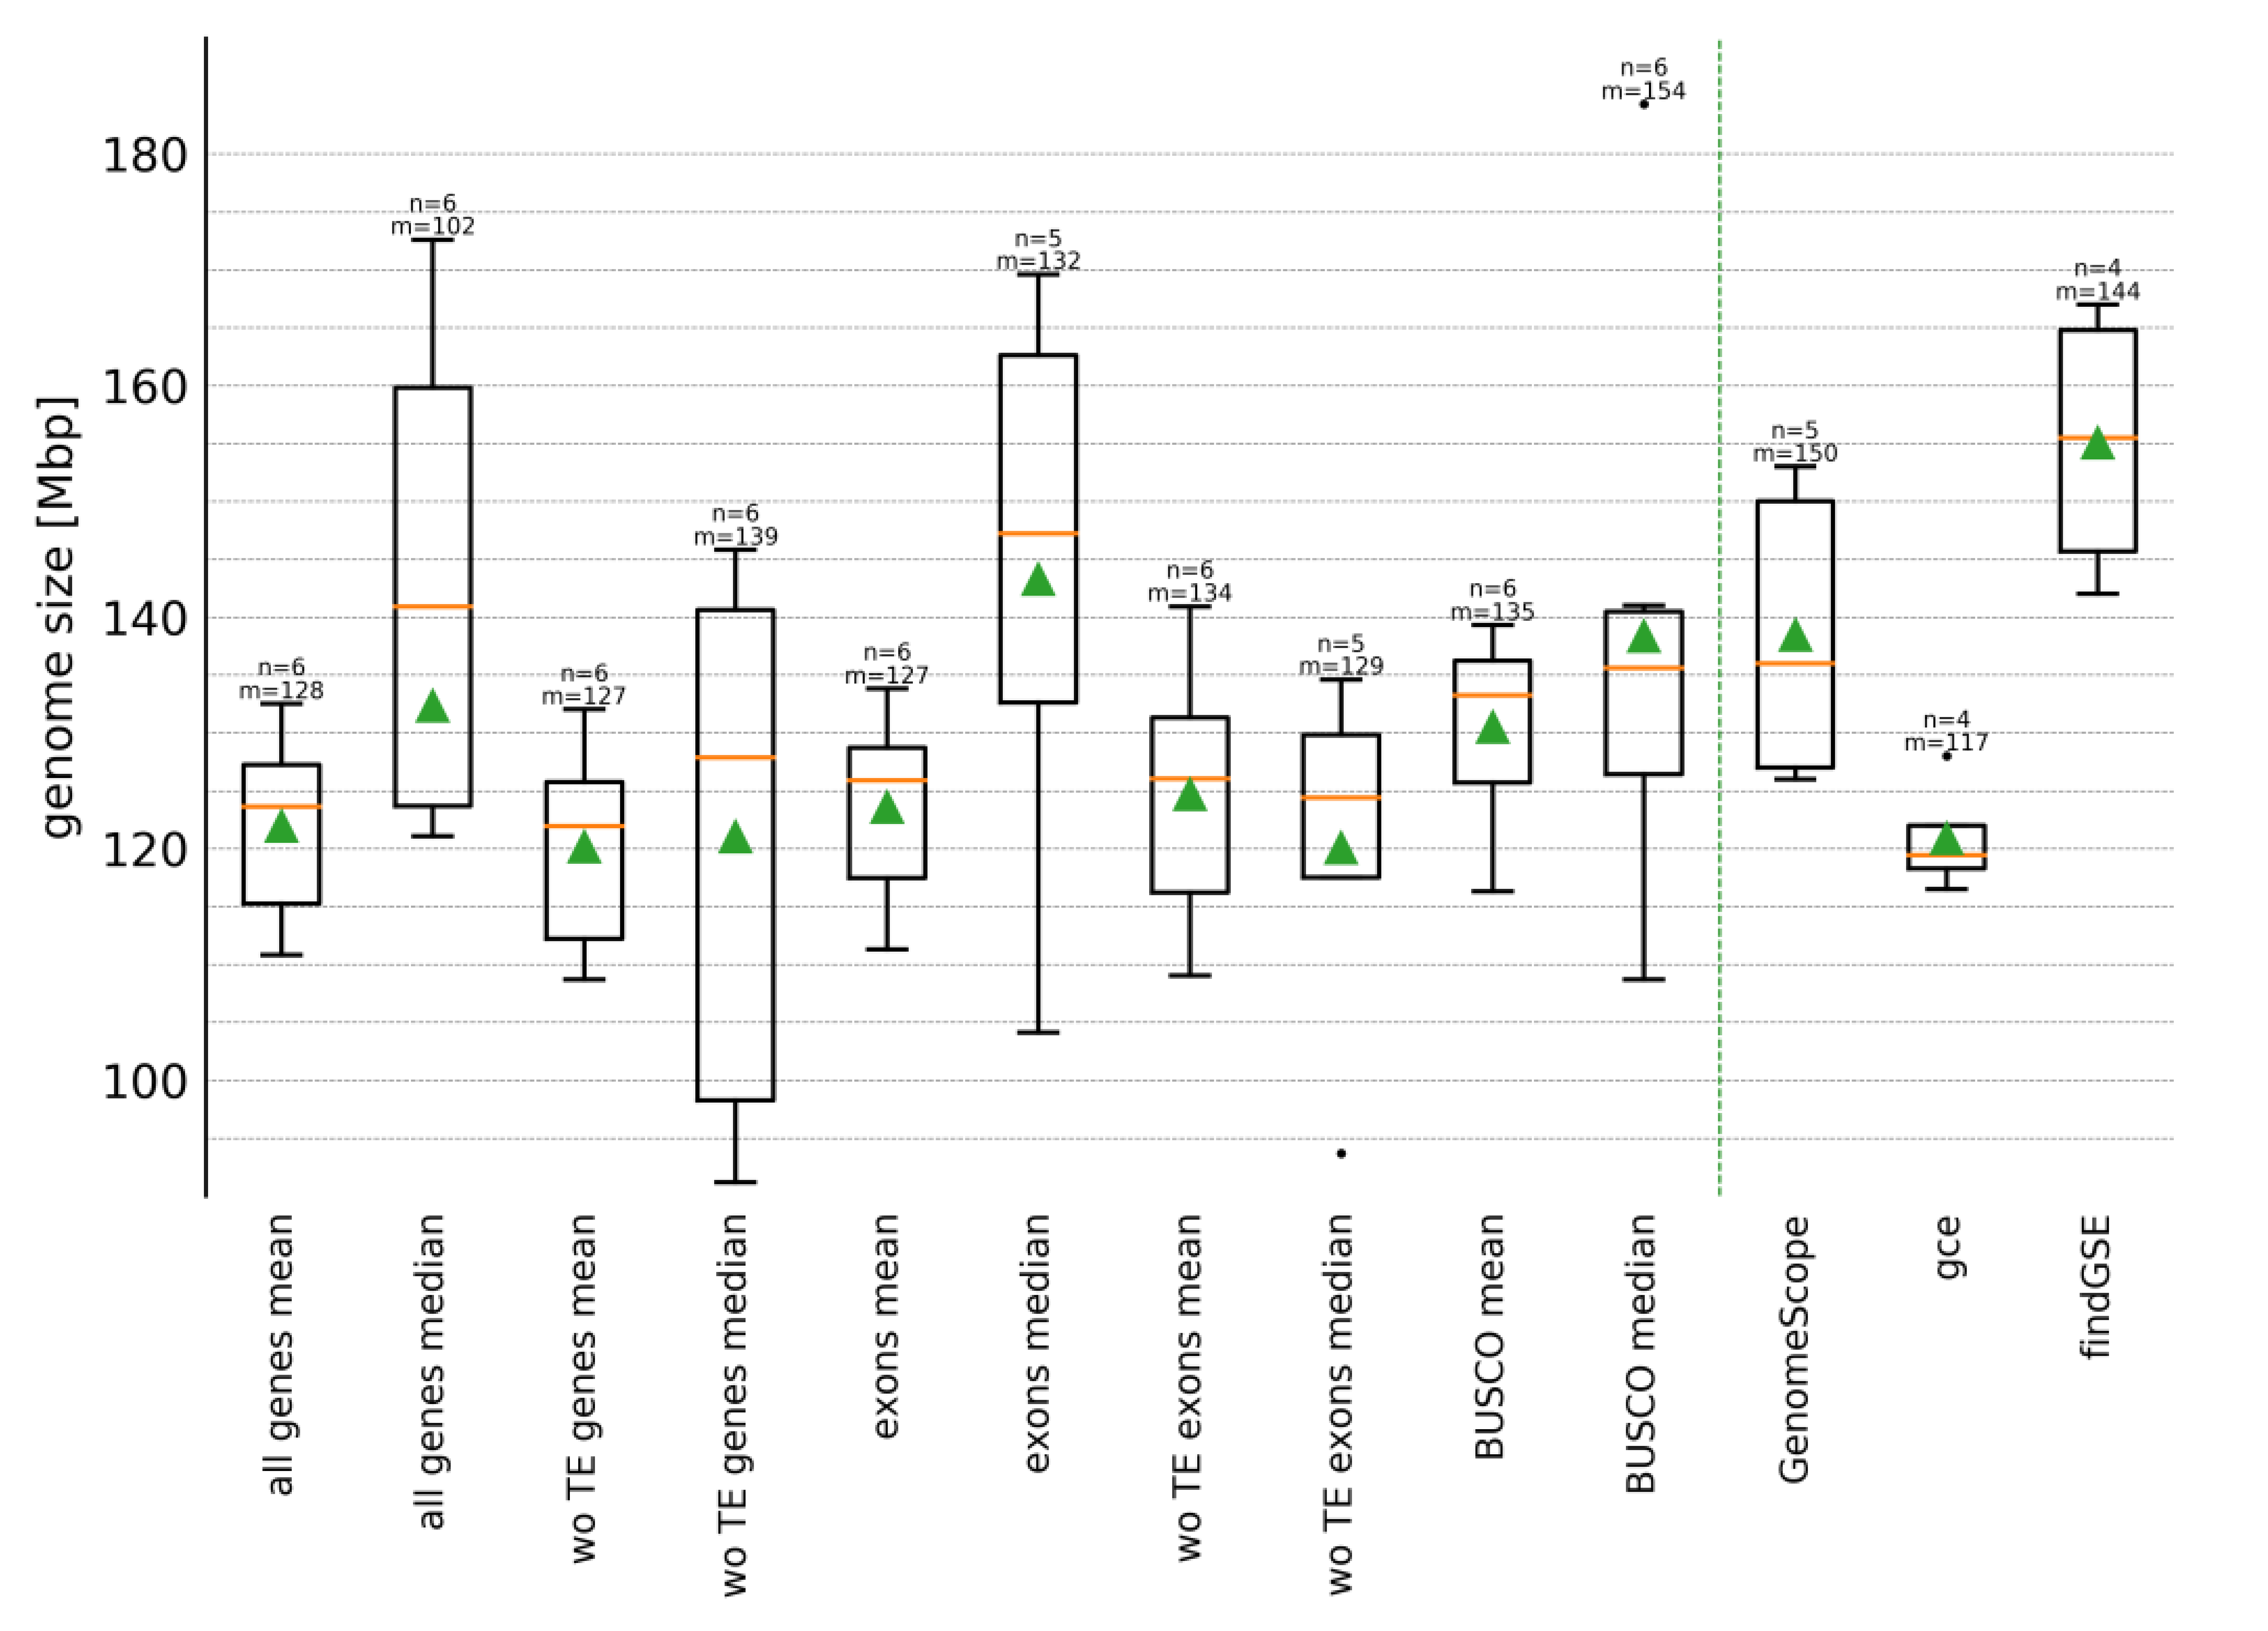
\includegraphics[width=0.7\textwidth]{capitoli/analisi/confronto/confronto2/1a.png}
		\caption{Dimensioni stimate dai metodi rispetto $n$ campioni di ecotipo Col-0 di \textit{A. thaliana}. Per il metodo MGSE vengono scelte la media o la mediana di porzioni diverse di genoma. La figura mostra per ciascun metodo il valor medio (in verde) e la mediana $m$ (in giallo).}
		\label{fig:2confronto1a}
	\end{figure}
		
	Nell'analisi dell'ecotipo Nd-1 mostrata dalla figura~\ref{fig:2confronto1b}, il metodo MGSE (sequenze BUSCO) mostra una differenza evidente nella stima della dimensione utilizzando la media o la mediana della copertura. Il valore stimato da MGSE attraverso la media delle sequenze BUSCO risulta il più affidabile, con una dimensione reale stimata di 138-140~Mb \cite{pucker2016denovo}. Mentre GCE restituisce un valore più plausibile, i metodi GenomeScope e findGSE generano una dimensione la cui correttezza risulta poco probabile.

	\begin{figure}[]
		\centering
		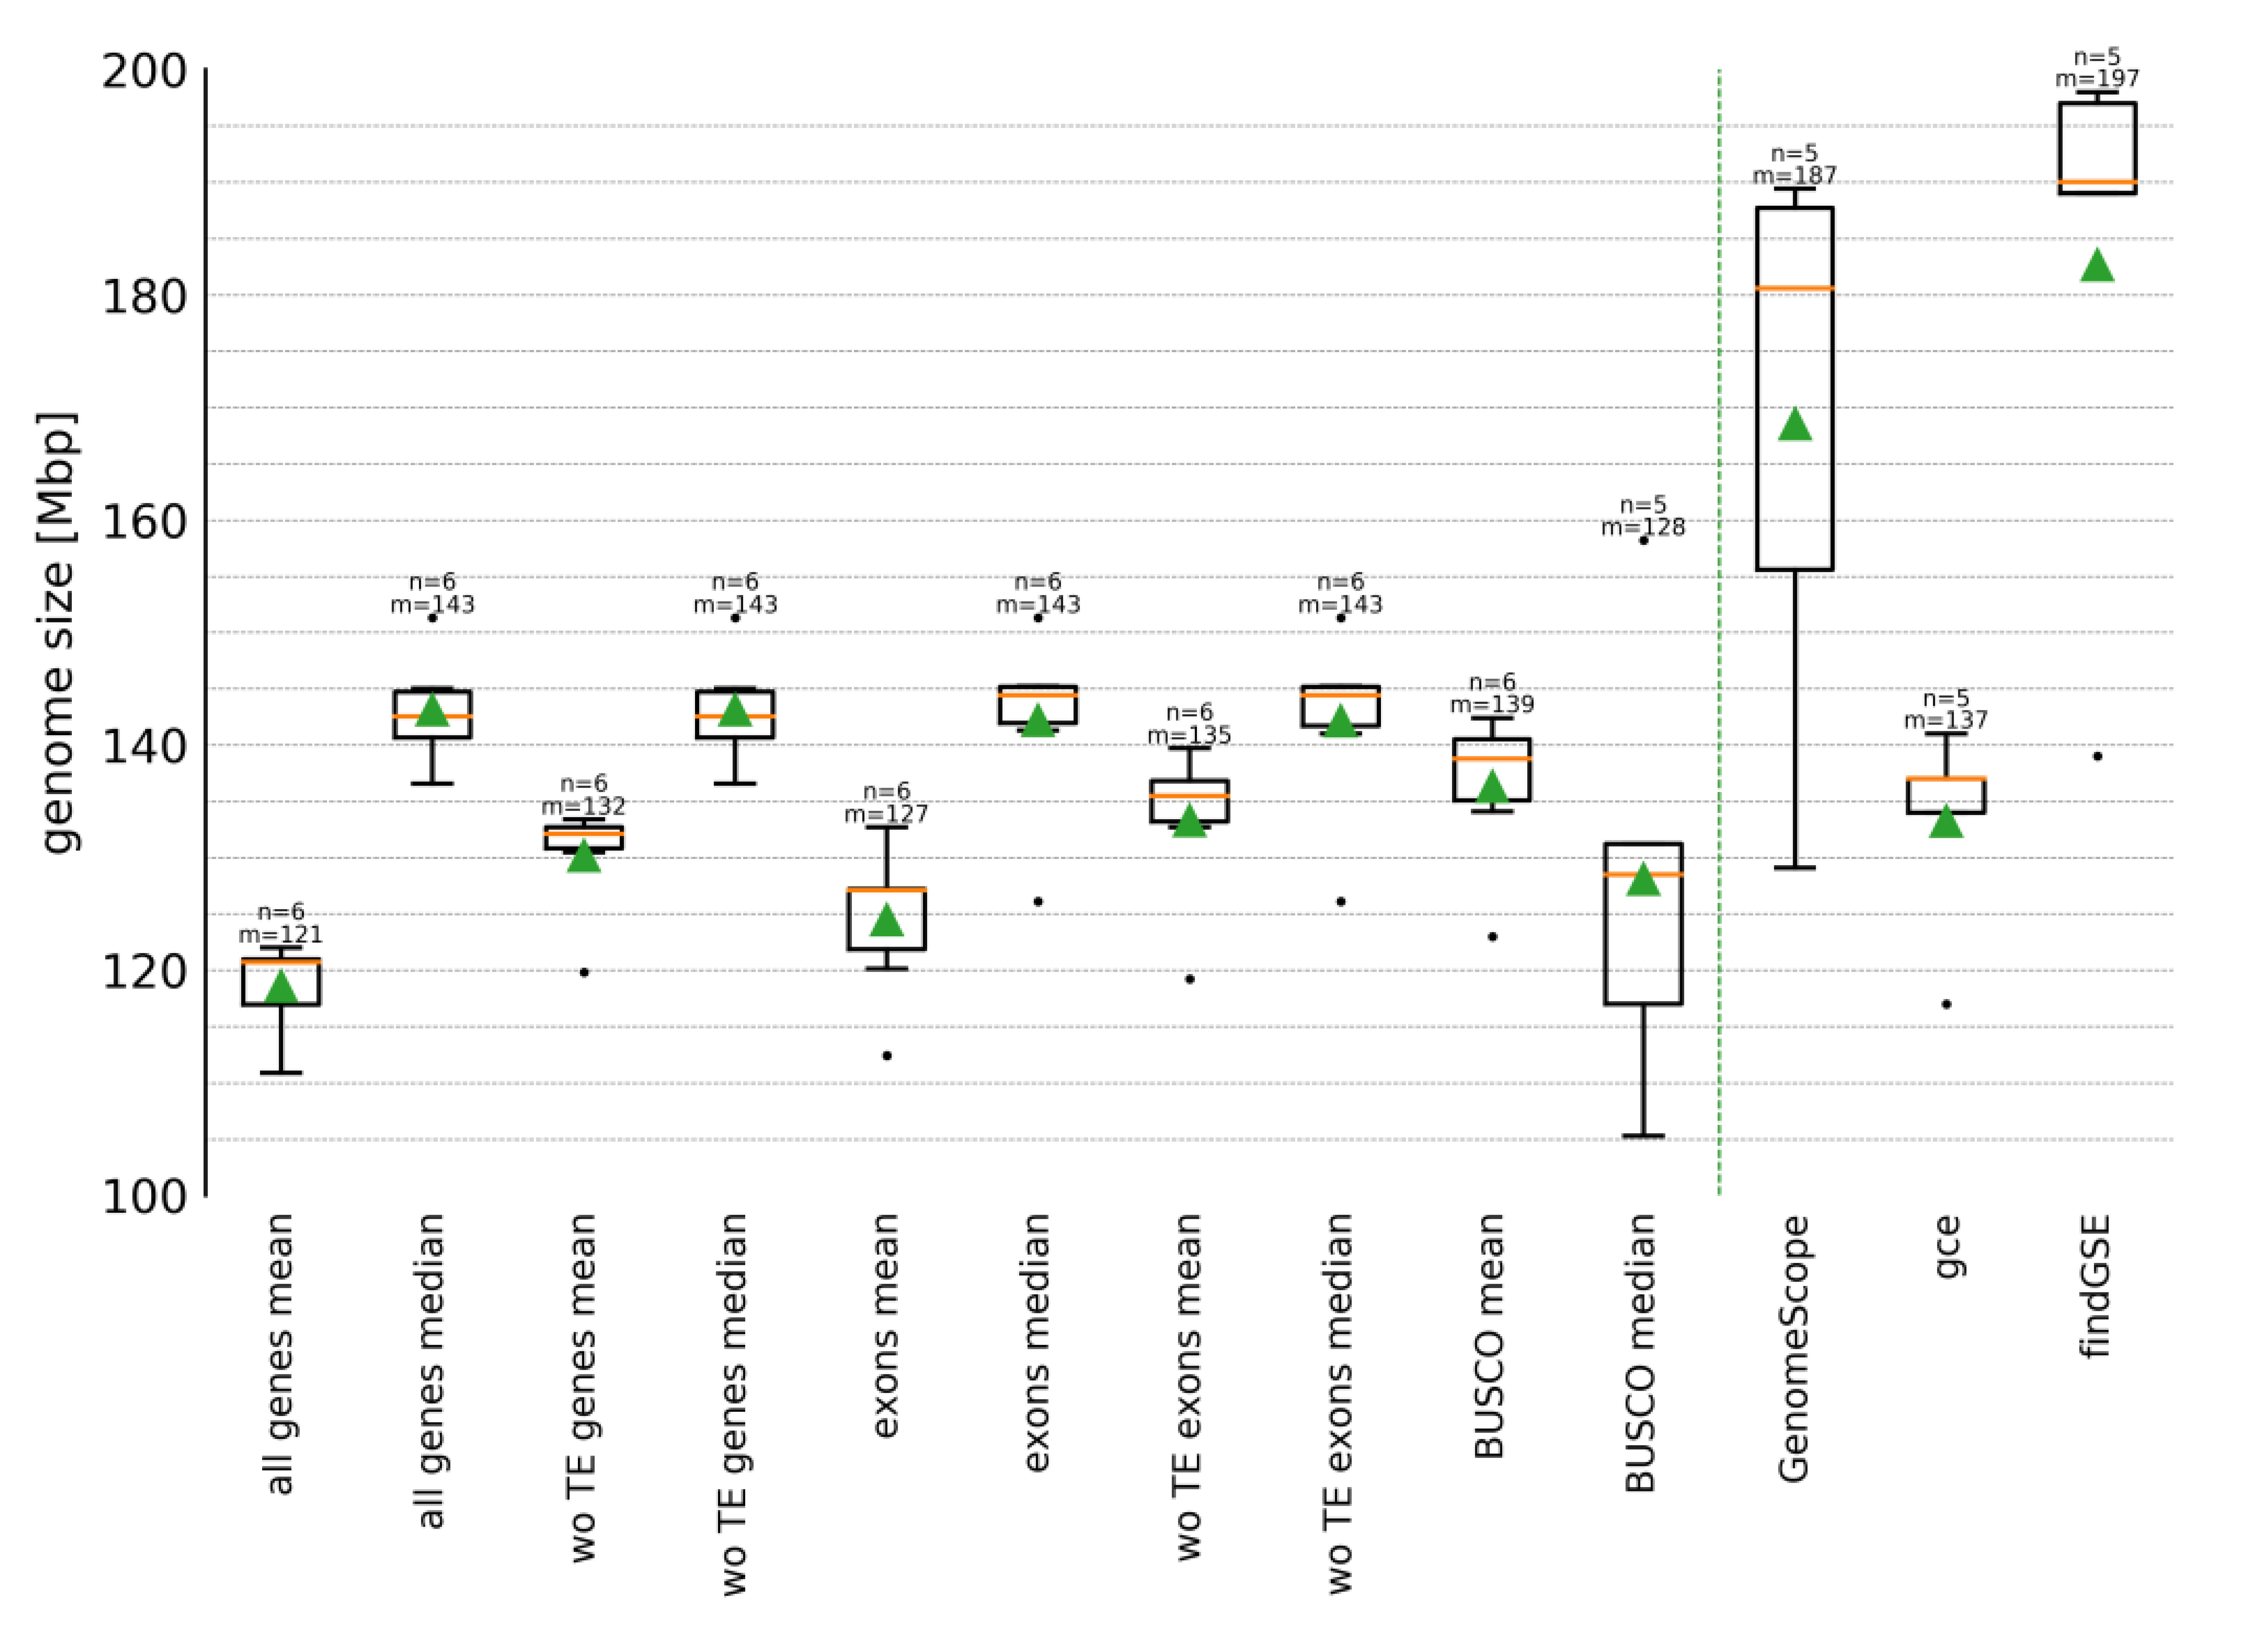
\includegraphics[width=0.7\textwidth]{capitoli/analisi/confronto/confronto2/1b.png}
		\caption{Dimensioni stimate dai metodi rispetto $n$ campioni di ecotipo Nd-1 di \textit{A. thaliana}. Per il metodo MGSE vengono scelte la media o la mediana di porzioni diverse di genoma. La figura mostra per ciascun metodo il valor medio (in verde) e la mediana $m$ (in giallo).}
		\label{fig:2confronto1b}
	\end{figure}
	
	Il confronto prosegue quindi con la stima della dimensione del genoma a partire da 1028 sequenze di \textit{A. thaliana}. I programmi GCE, GenomeScope e findGSE nella maggior parte dei casi stimano valori compresi tra 120 e 200 Mb, mentre MGSE tra 120 e 160 Mb, come mostrato nella figura~\vref{fig:2confronto3}. Si riporta comunque che tutti i metodi hanno generano alcuni valori errati, estremamente elevati o ridotti. In media, findGSE tende a stimare valori maggiori rispetto agli altri metodi basati sui k-mer.
	
	\begin{figure}[]
		\centering
		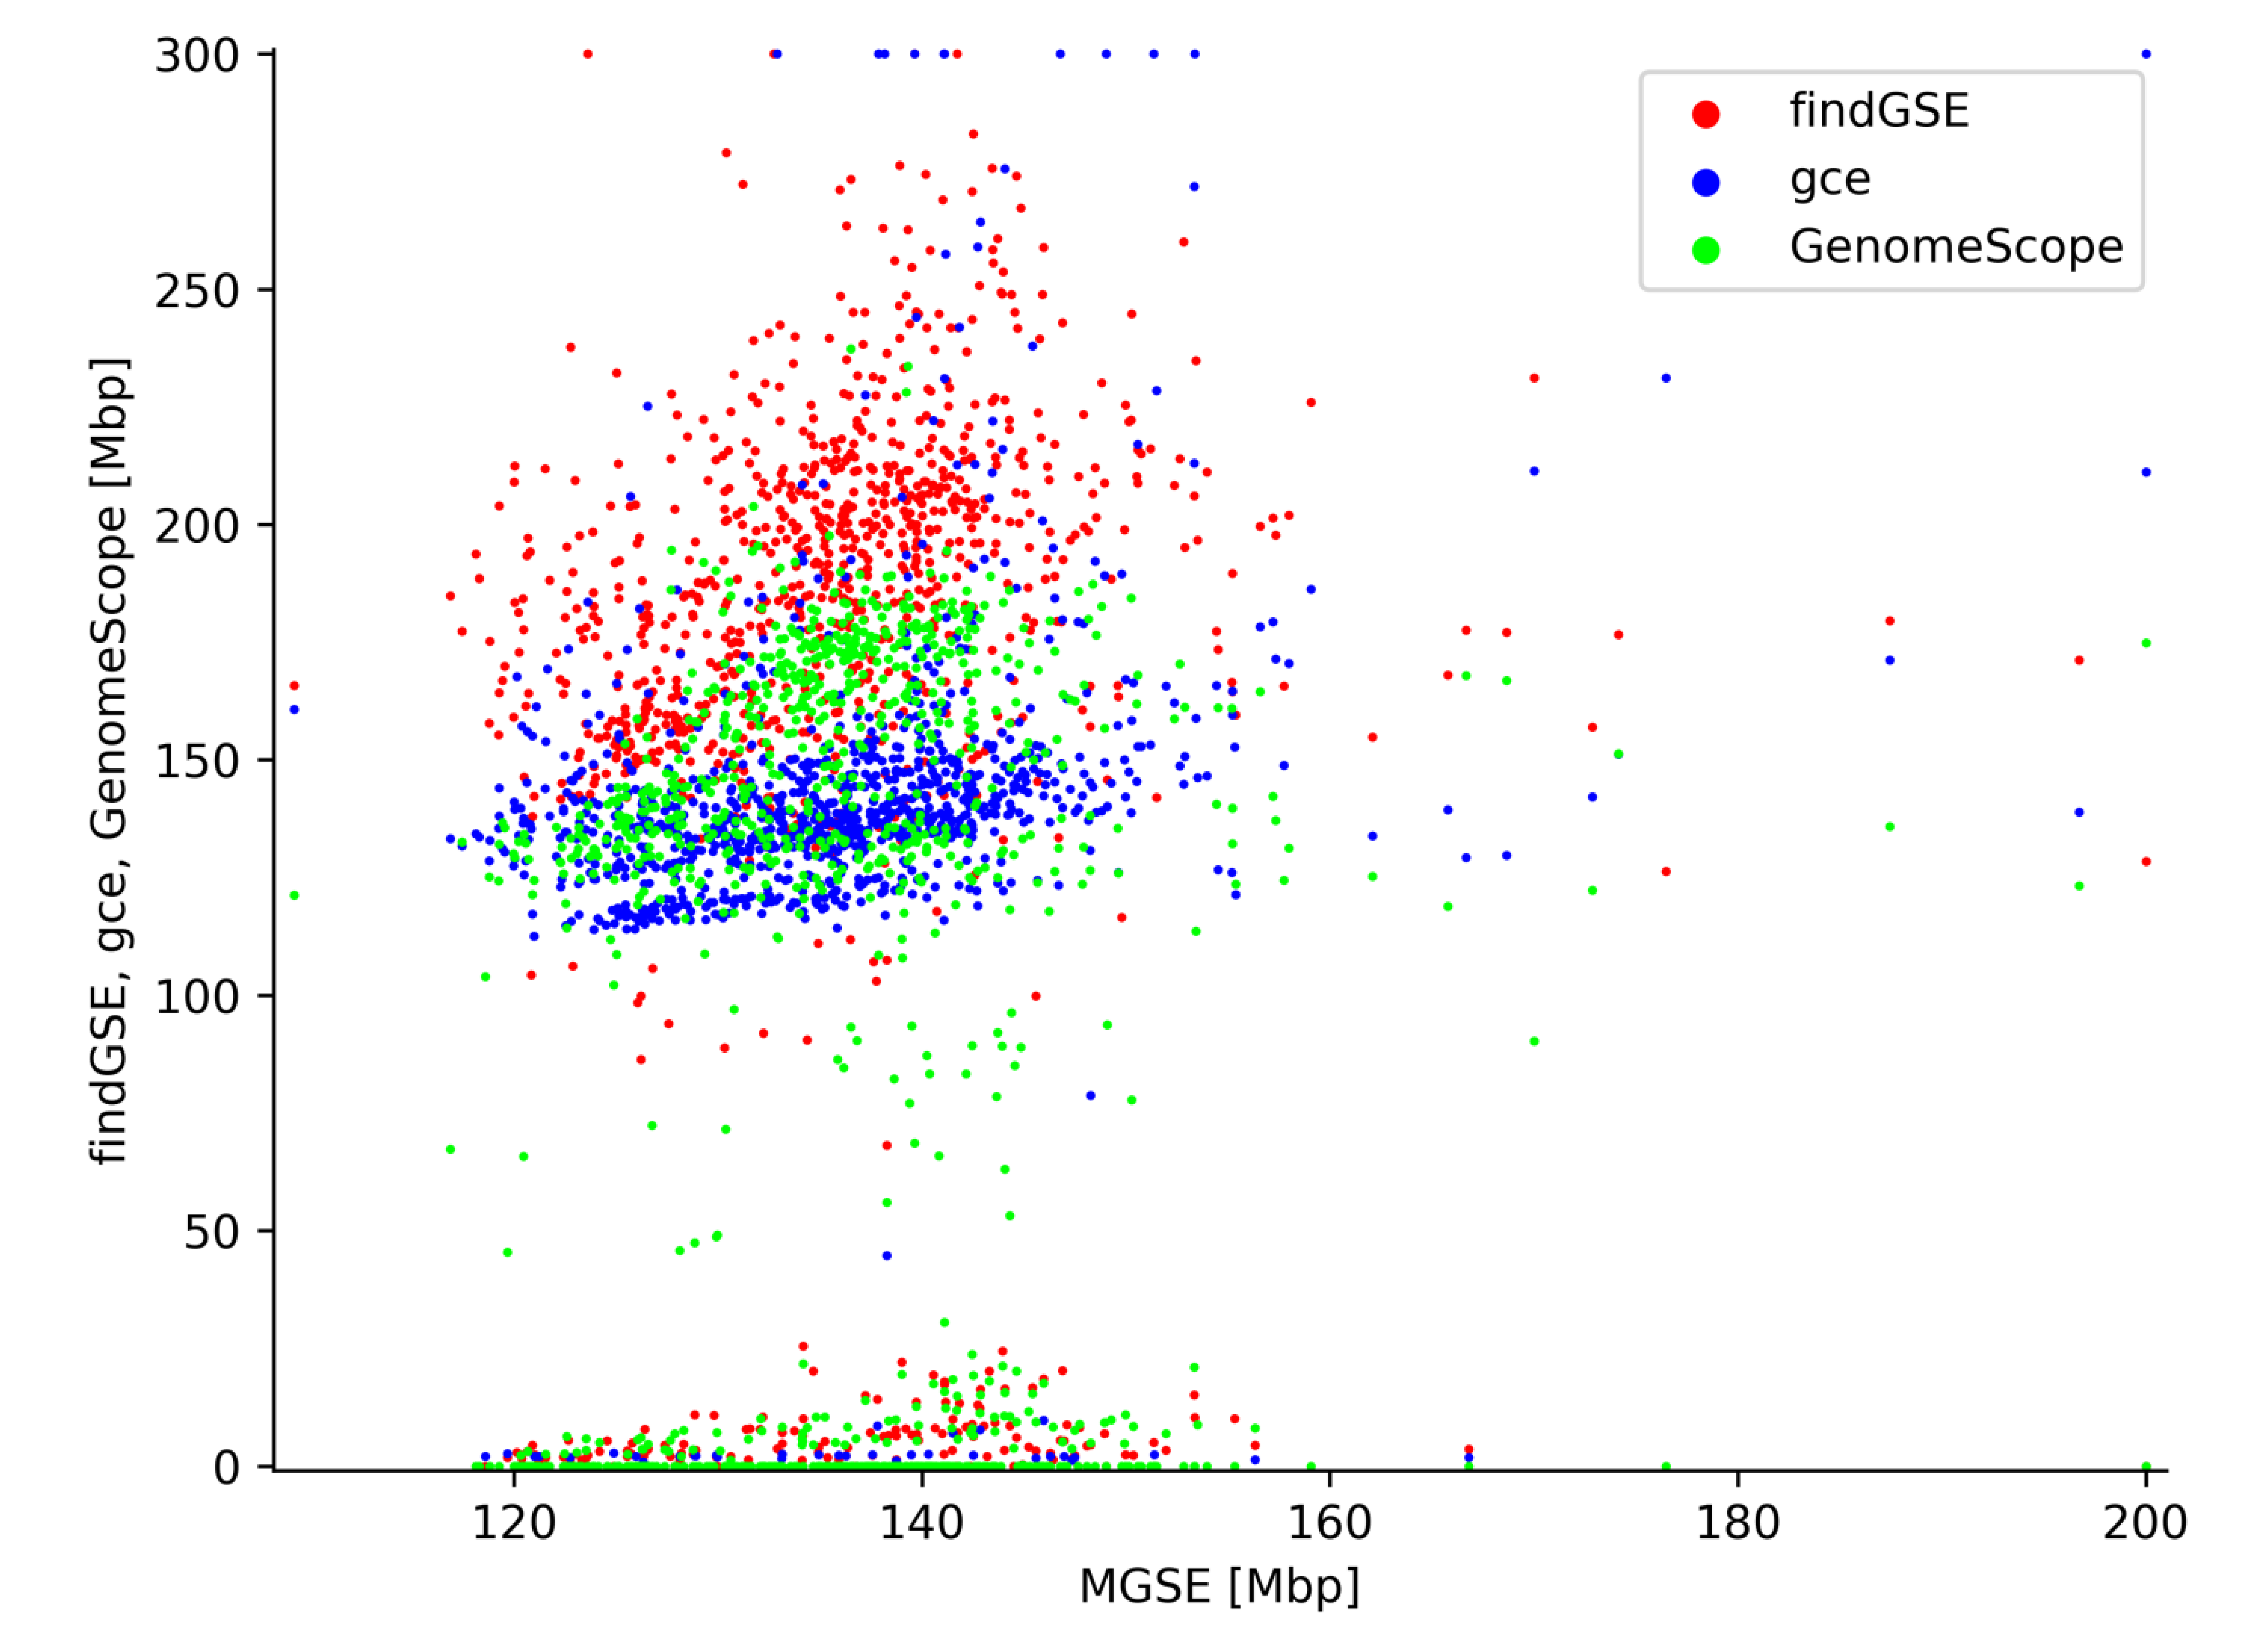
\includegraphics[width=0.7\textwidth]{capitoli/analisi/confronto/confronto2/2.png}
		\caption{Stima della dimensione di 1028 sequenze di \textit{A. thaliana}. I risultati metodi findGSE, GCE e GenomeScope vengono mostrati in funzione delle stime del metodo MGSE. Eventuali outlier vengono rappresentati sul bordo del grafico, permettendo una maggiore risoluzione alla nuvola centrale.}
		\label{fig:2confronto3}
	\end{figure} 

	\paragraph{Stima della dimensione di \textit{Beta vulgaris}}
	Per verificare l'accuratezza nella stima di genomi con maggiori dimensioni e complessità, i programmi vengono utilizzati per determinare la dimensione di \textit{Beta vulgaris}. Dato che vengono utilizzate sequenze diverse come dati iniziali, sono attese differenze minime tra le letture di input, che potrebbero far variare i valori stimati dai metodi. Comunque, dato che al momento del test l'assembly più sviluppato del genoma di tale specie comprende 567 Mb della sequenza completa, i valori minori di tale soglia possono essere classificati come erronei. 
	
	Come mostrato dalla figura~\vref{fig:2confronto4}, i metodi GenomeScope e GCE tendono a sottodimensionare la stima, restituendo valori in media di 500 Mb. Il programma findGSE, invece, genera risultati ad alta variabilità. Il metodo MGSE, utilizzando la media della copertura dei geni a singola copia o delle regioni BUSCO, sembra avere prestazioni migliori.
	
	\begin{figure}[]
		\centering
		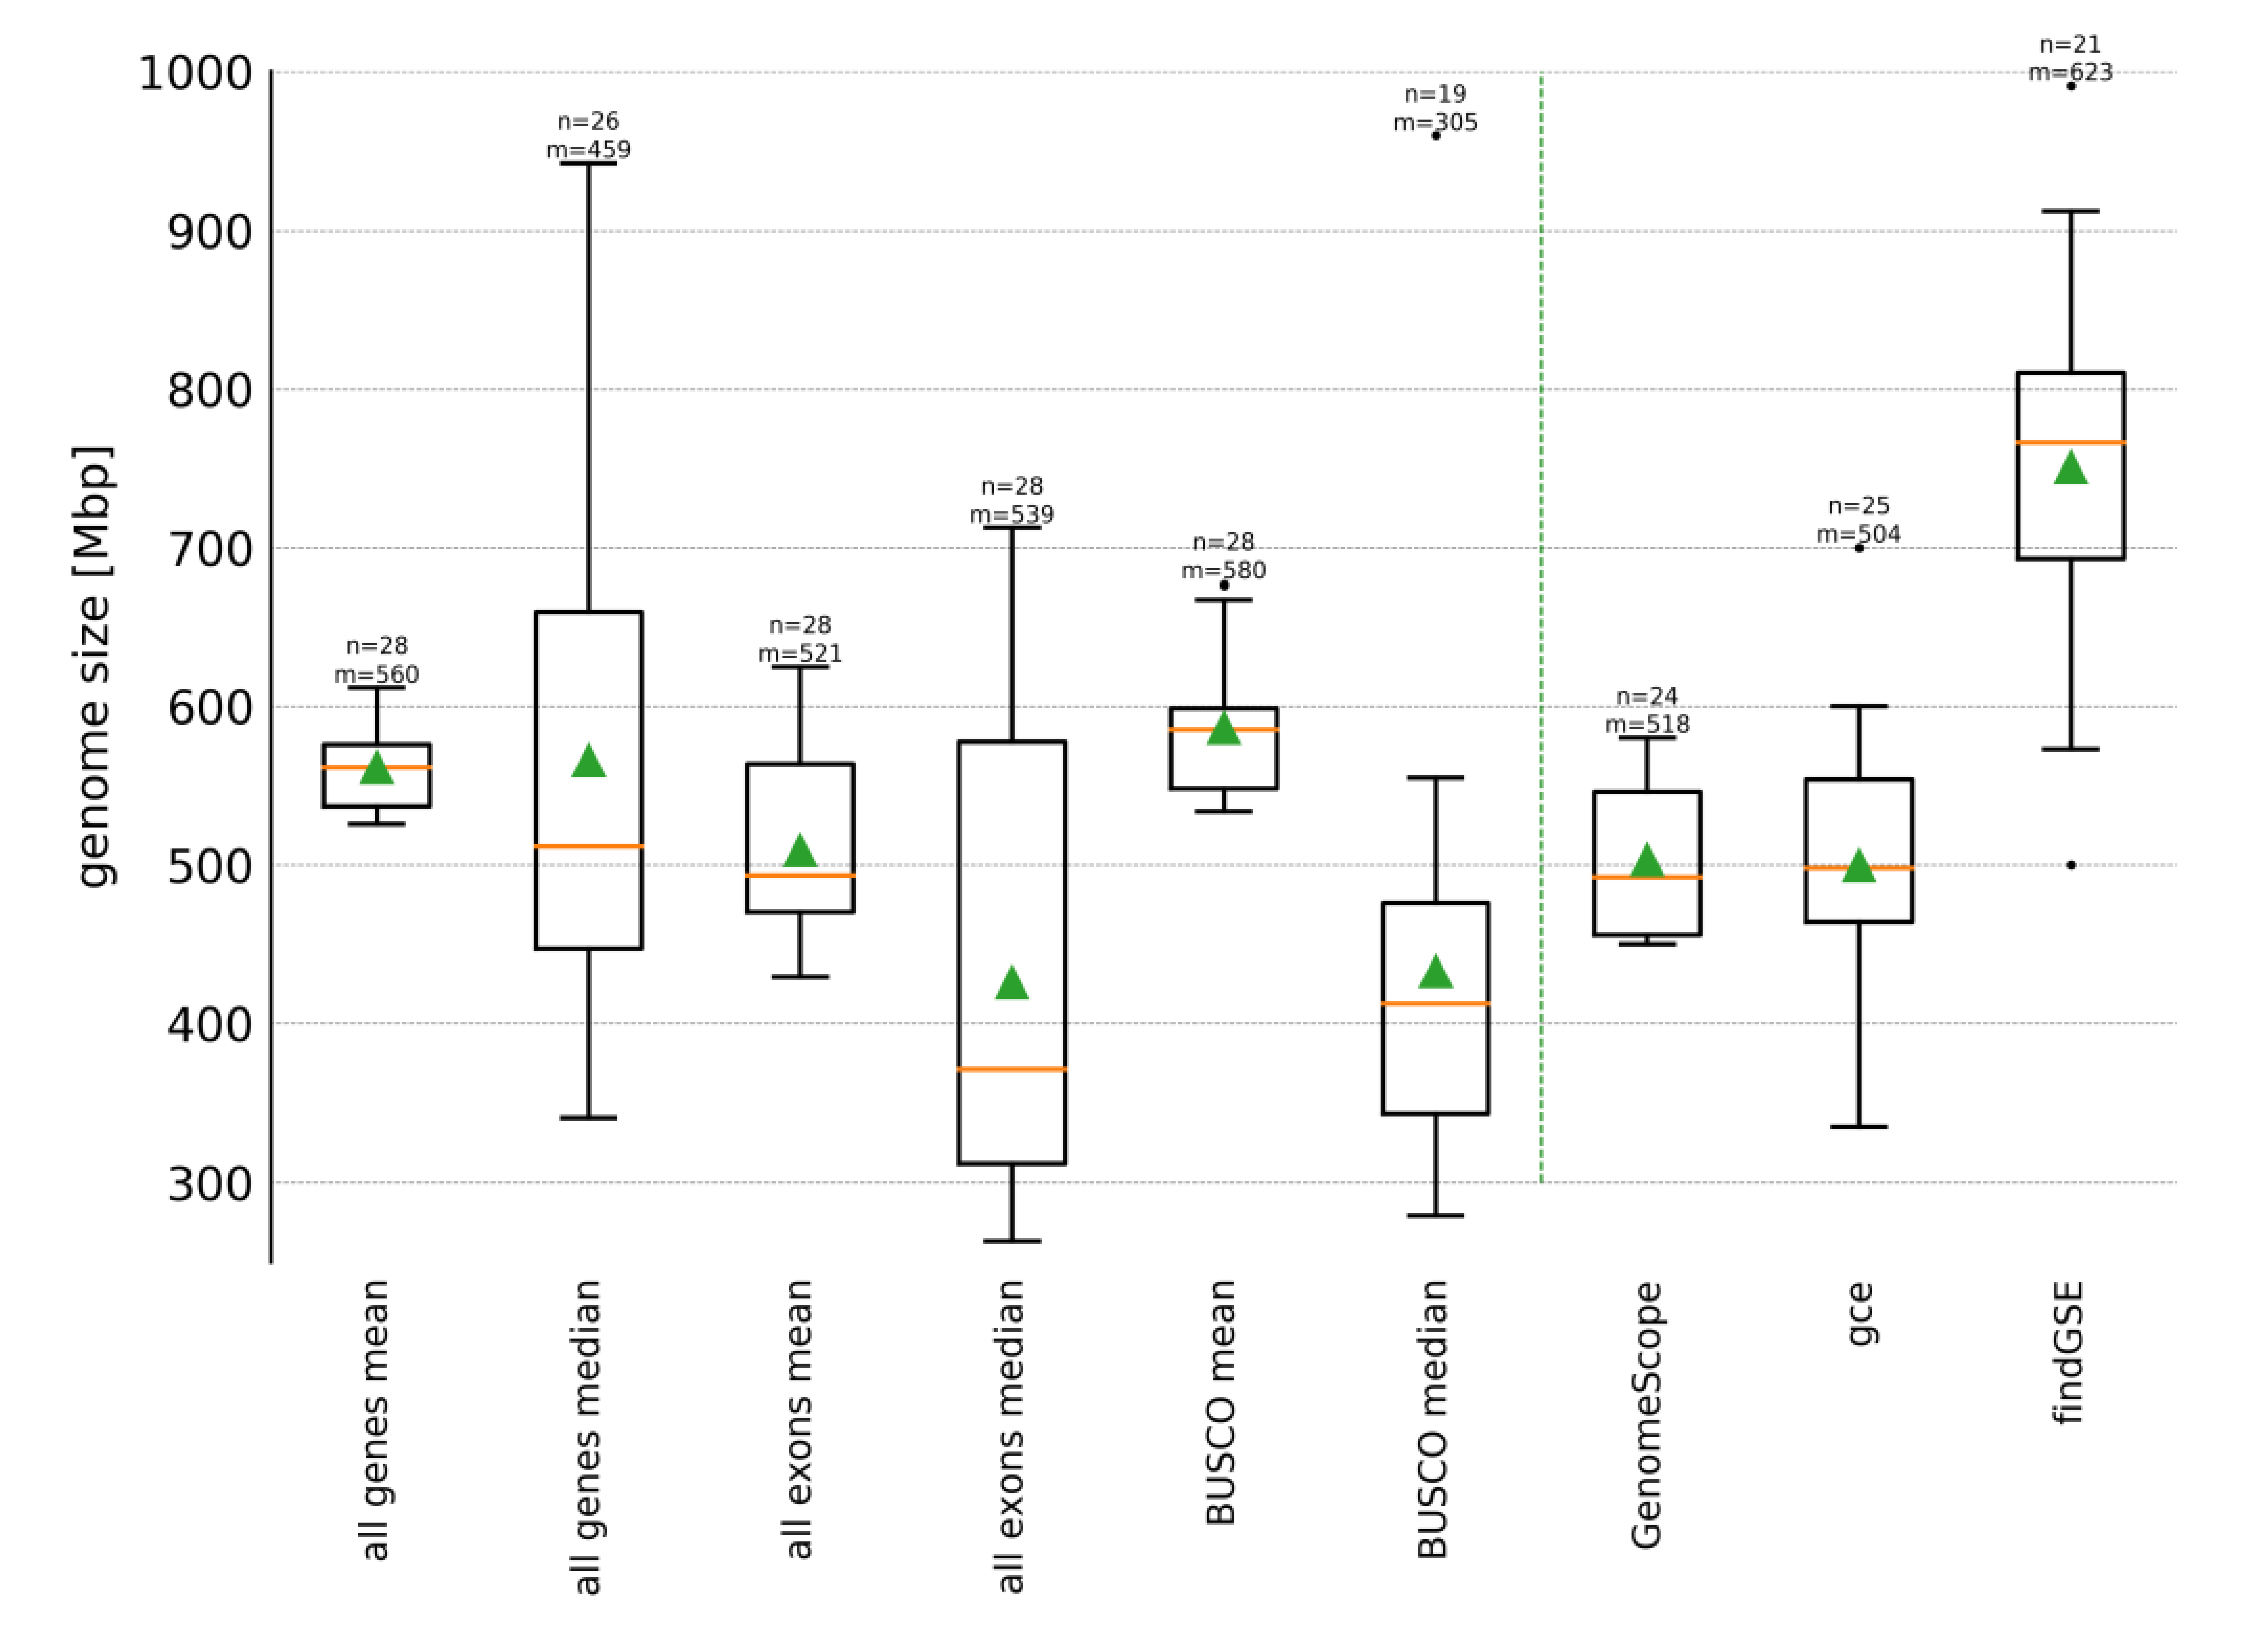
\includegraphics[width=0.7\textwidth]{capitoli/analisi/confronto/confronto2/3.png}
		\caption{Dimensioni stimate dai metodi rispetto $n$ campioni di \textit{Beta vulgaris}. Per il metodo MGSE vengono scelte la media o la mediana di porzioni diverse di genoma. La figura mostra per ciascun metodo il valor medio (in verde) e la mediana $m$ (in giallo).}
		\label{fig:2confronto4}
	\end{figure} 

	\paragraph{Dimensione di genomi di altre specie}
	L'analisi continua con la stima delle dimensioni di genomi di varie specie, ciascuna con caratteristiche diverse: il \textit{Brachypodium distachyon} come modello di pianta erbacea, il pomodoro (\textit{Solanum lycopersicum}) per il clade delle Asteridi, il mais (\textit{Zea mays}) è stato incluso come specie monocotiledone ad alto contenuto di trasposoni, e la vite comune (\textit{Vitis vinifera}) per la sua elevata eterozigosi.
	
	I programmi, come mostrato dalla figura~\vref{fig:2confronto5}, restituiscono generalmente risultati appartenenti al medesimo intervallo. Nella stima della dimensione di \textit{B. distachyon}, mentre MGSE, GenomeScope e GCE tendono a generare valori non corretti, findGSE stima una previsione ragionevole di 303 Mb, a fronte di una lunghezza stimata di circa 355 Mb \cite{ozdemir2008brachypodium}. 
	La dimensione del genoma di \textit{Z. mays} è ampiamente sottostimata da tutti i programmi, dato che la lunghezza stimata risulta di 2.4 Gb \cite{haberer2005structure}. 
	A differenza di MGSE e GCE, i programmi findGSE e GenomeScope stimano correttamente la lunghezza attesa di \textit{S. lycopersicum} (950 Mb \cite{barone2008structural}).	
	A causa dell'alta eterozigosi, MGSE restituisce un valore di soli 50 Mbp per il genoma di \textit{V. vinifera}, mentre il programma GenomeScope restituisce un valore plausibile, avendo una dimensione stimata è di 475~Mb~\cite{myles2010rapid}.

	\begin{figure}
		\centering
		\subfloat[][\emph{Stima della dimensione del genoma di specie \textit{Brachypodium distachyon}.}]
			{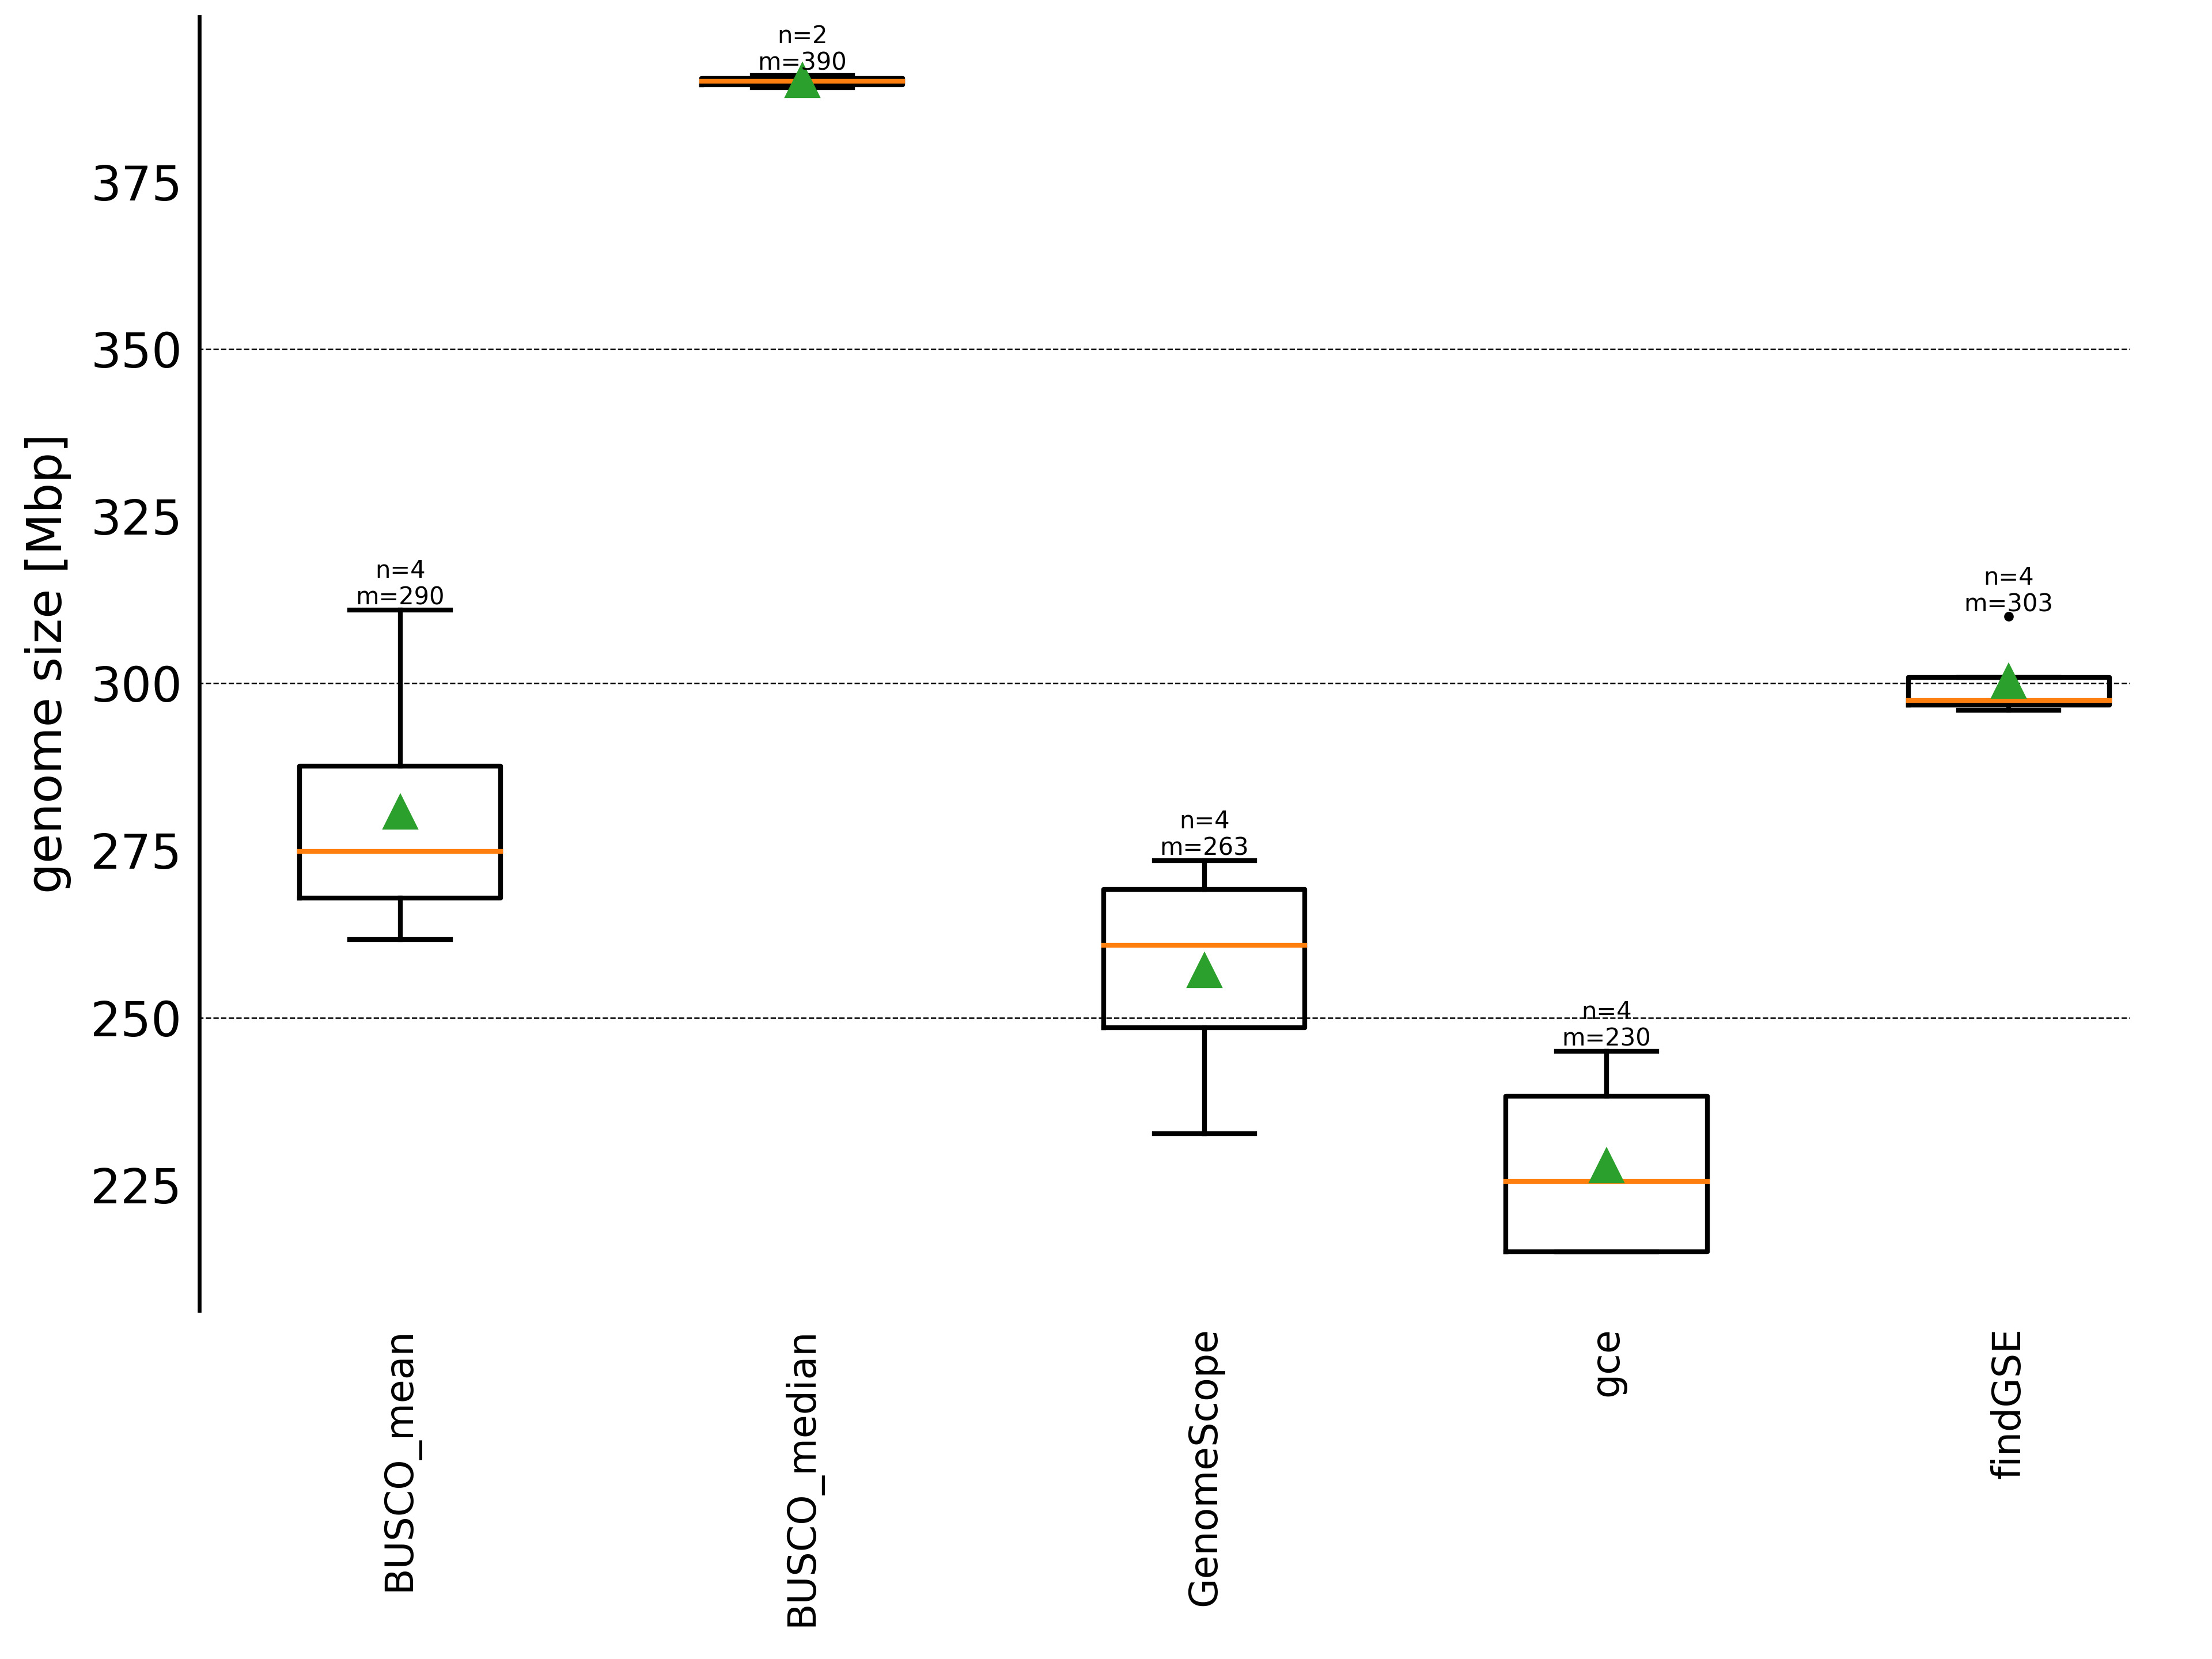
\includegraphics[width=0.45\textwidth]{capitoli/analisi/confronto/confronto2/6.jpg}} \quad
		\subfloat[][\emph{Stima della dimensione del genoma di specie \textit{Zea mays}.}]
			{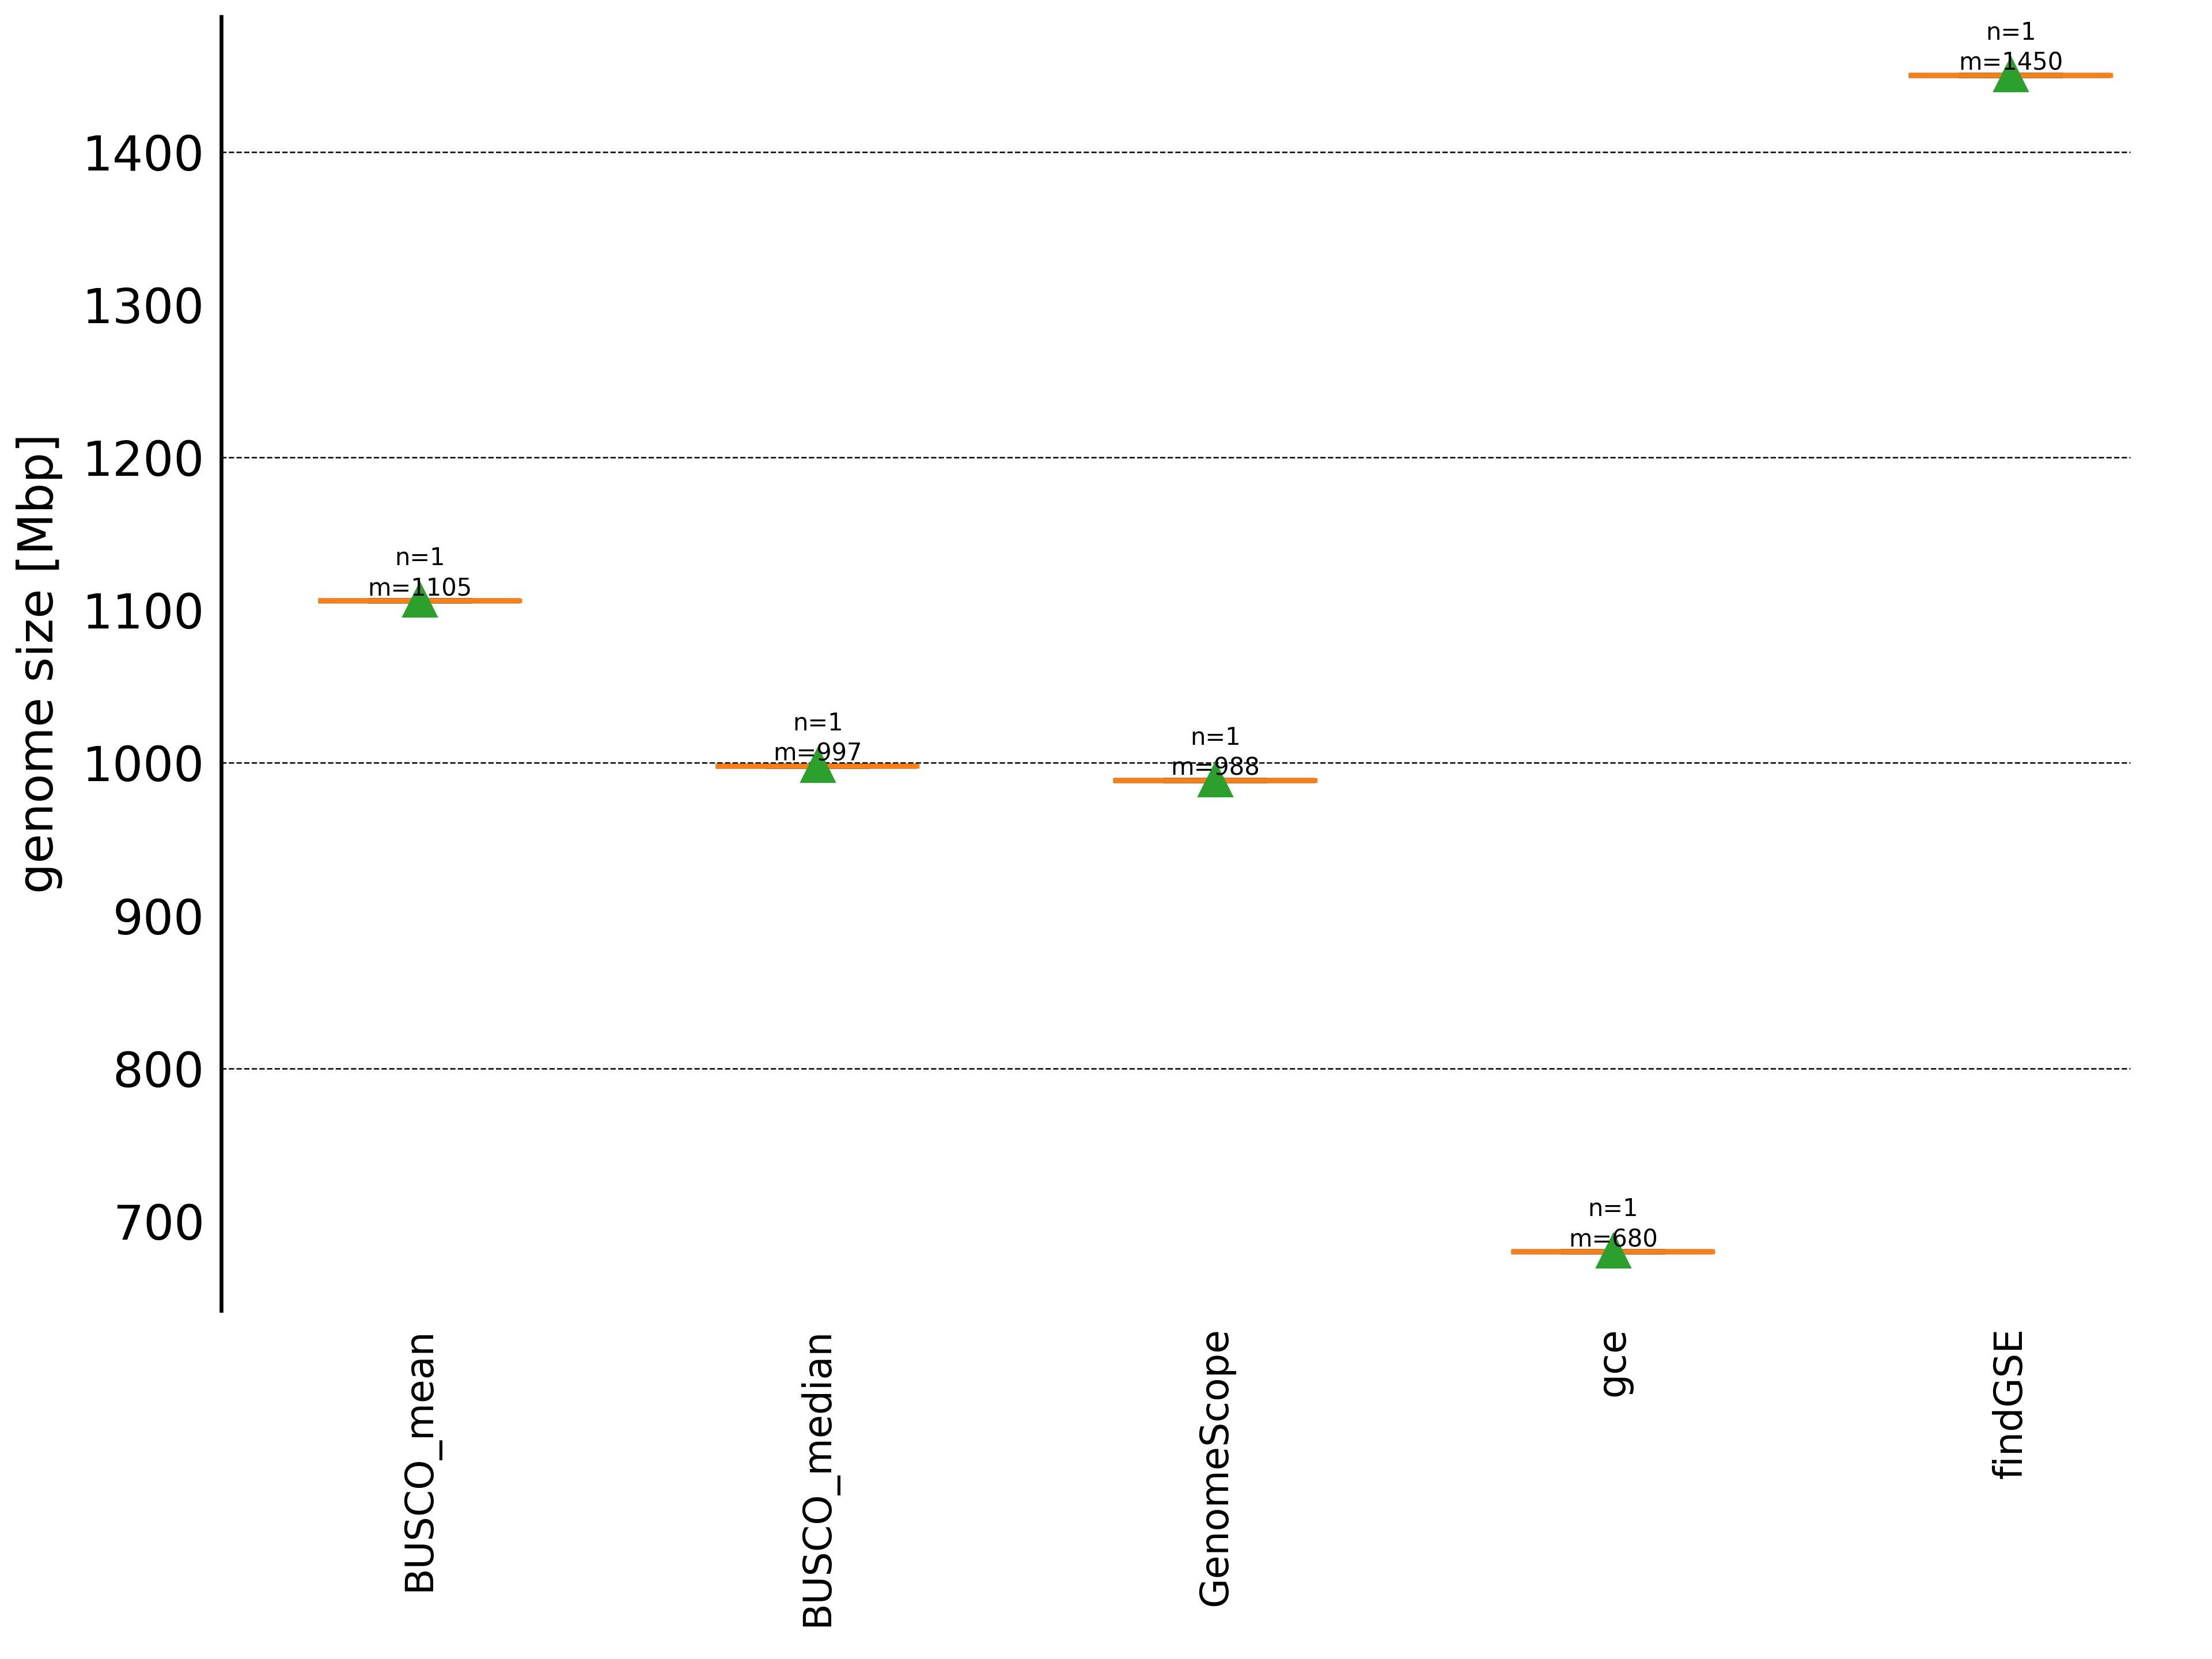
\includegraphics[width=0.45\textwidth]{capitoli/analisi/confronto/confronto2/7.jpg}} \\ 
		\subfloat[][\emph{Stima della dimensione del genoma di specie \textit{Solanum lycopersicum}.}]
			{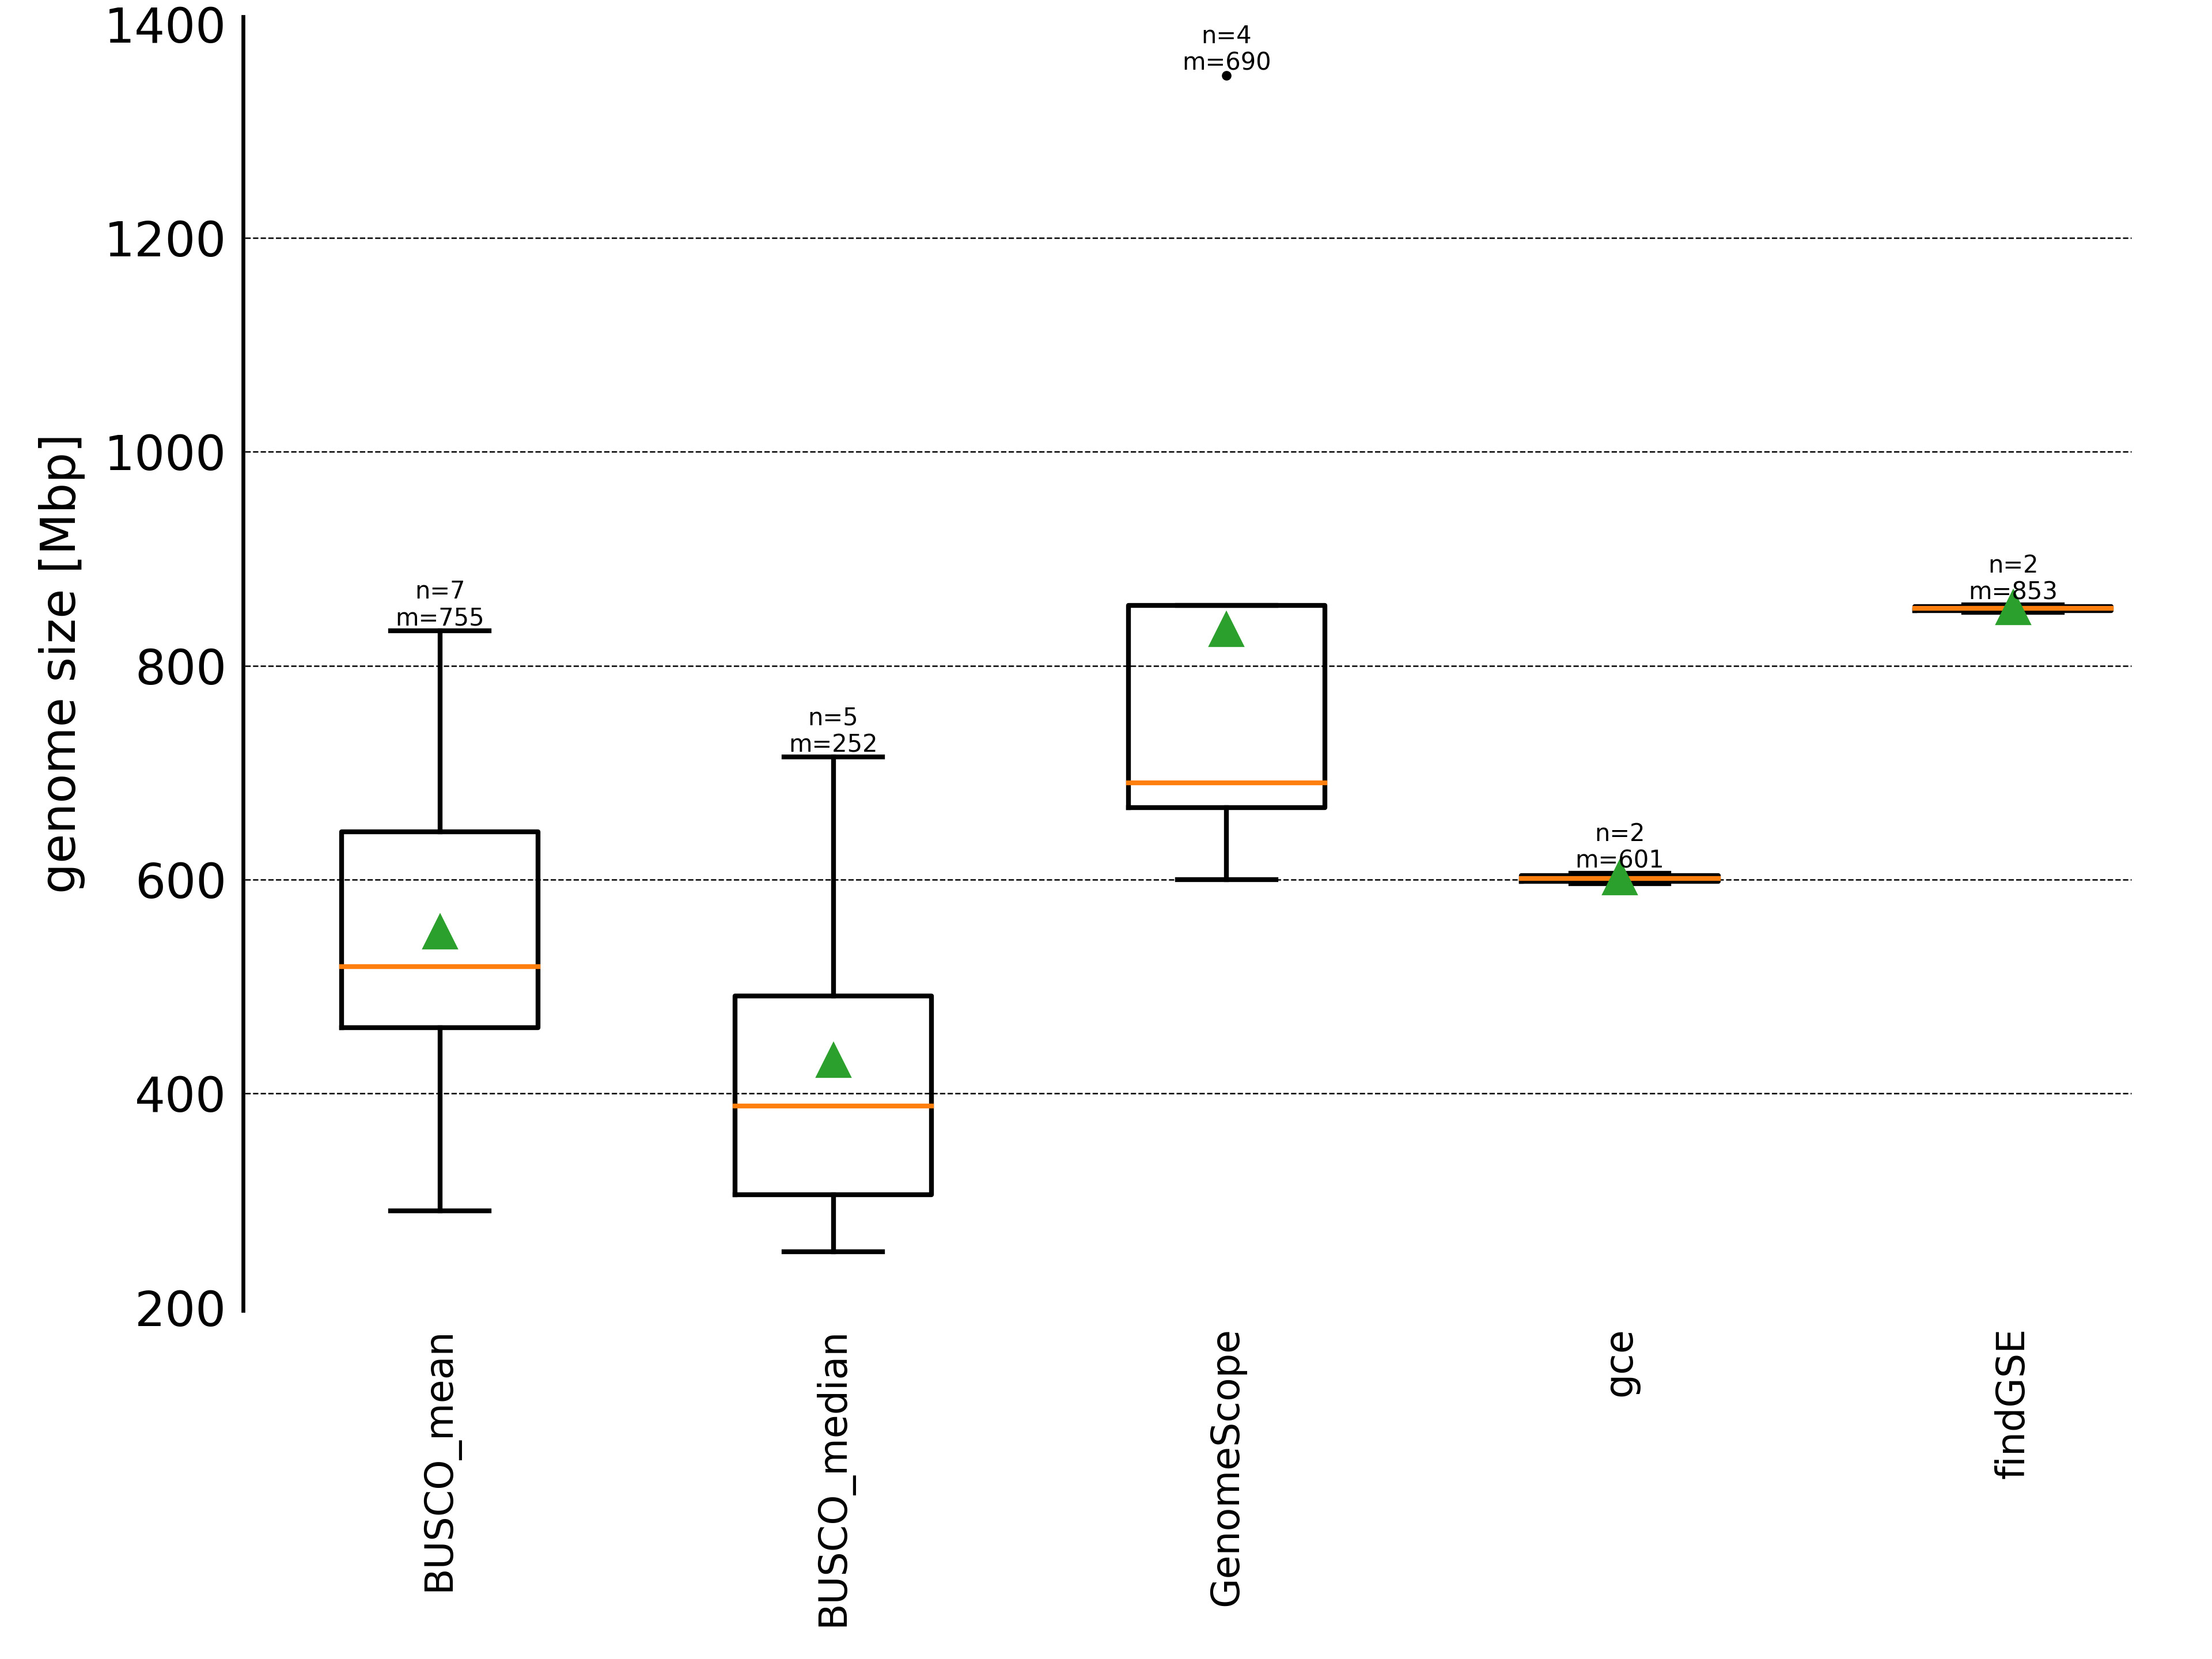
\includegraphics[width=0.45\textwidth]{capitoli/analisi/confronto/confronto2/8.jpg}} \quad
		\subfloat[][\emph{Stima della dimensione del genoma di specie \textit{Vitis vinifera}.}]
			{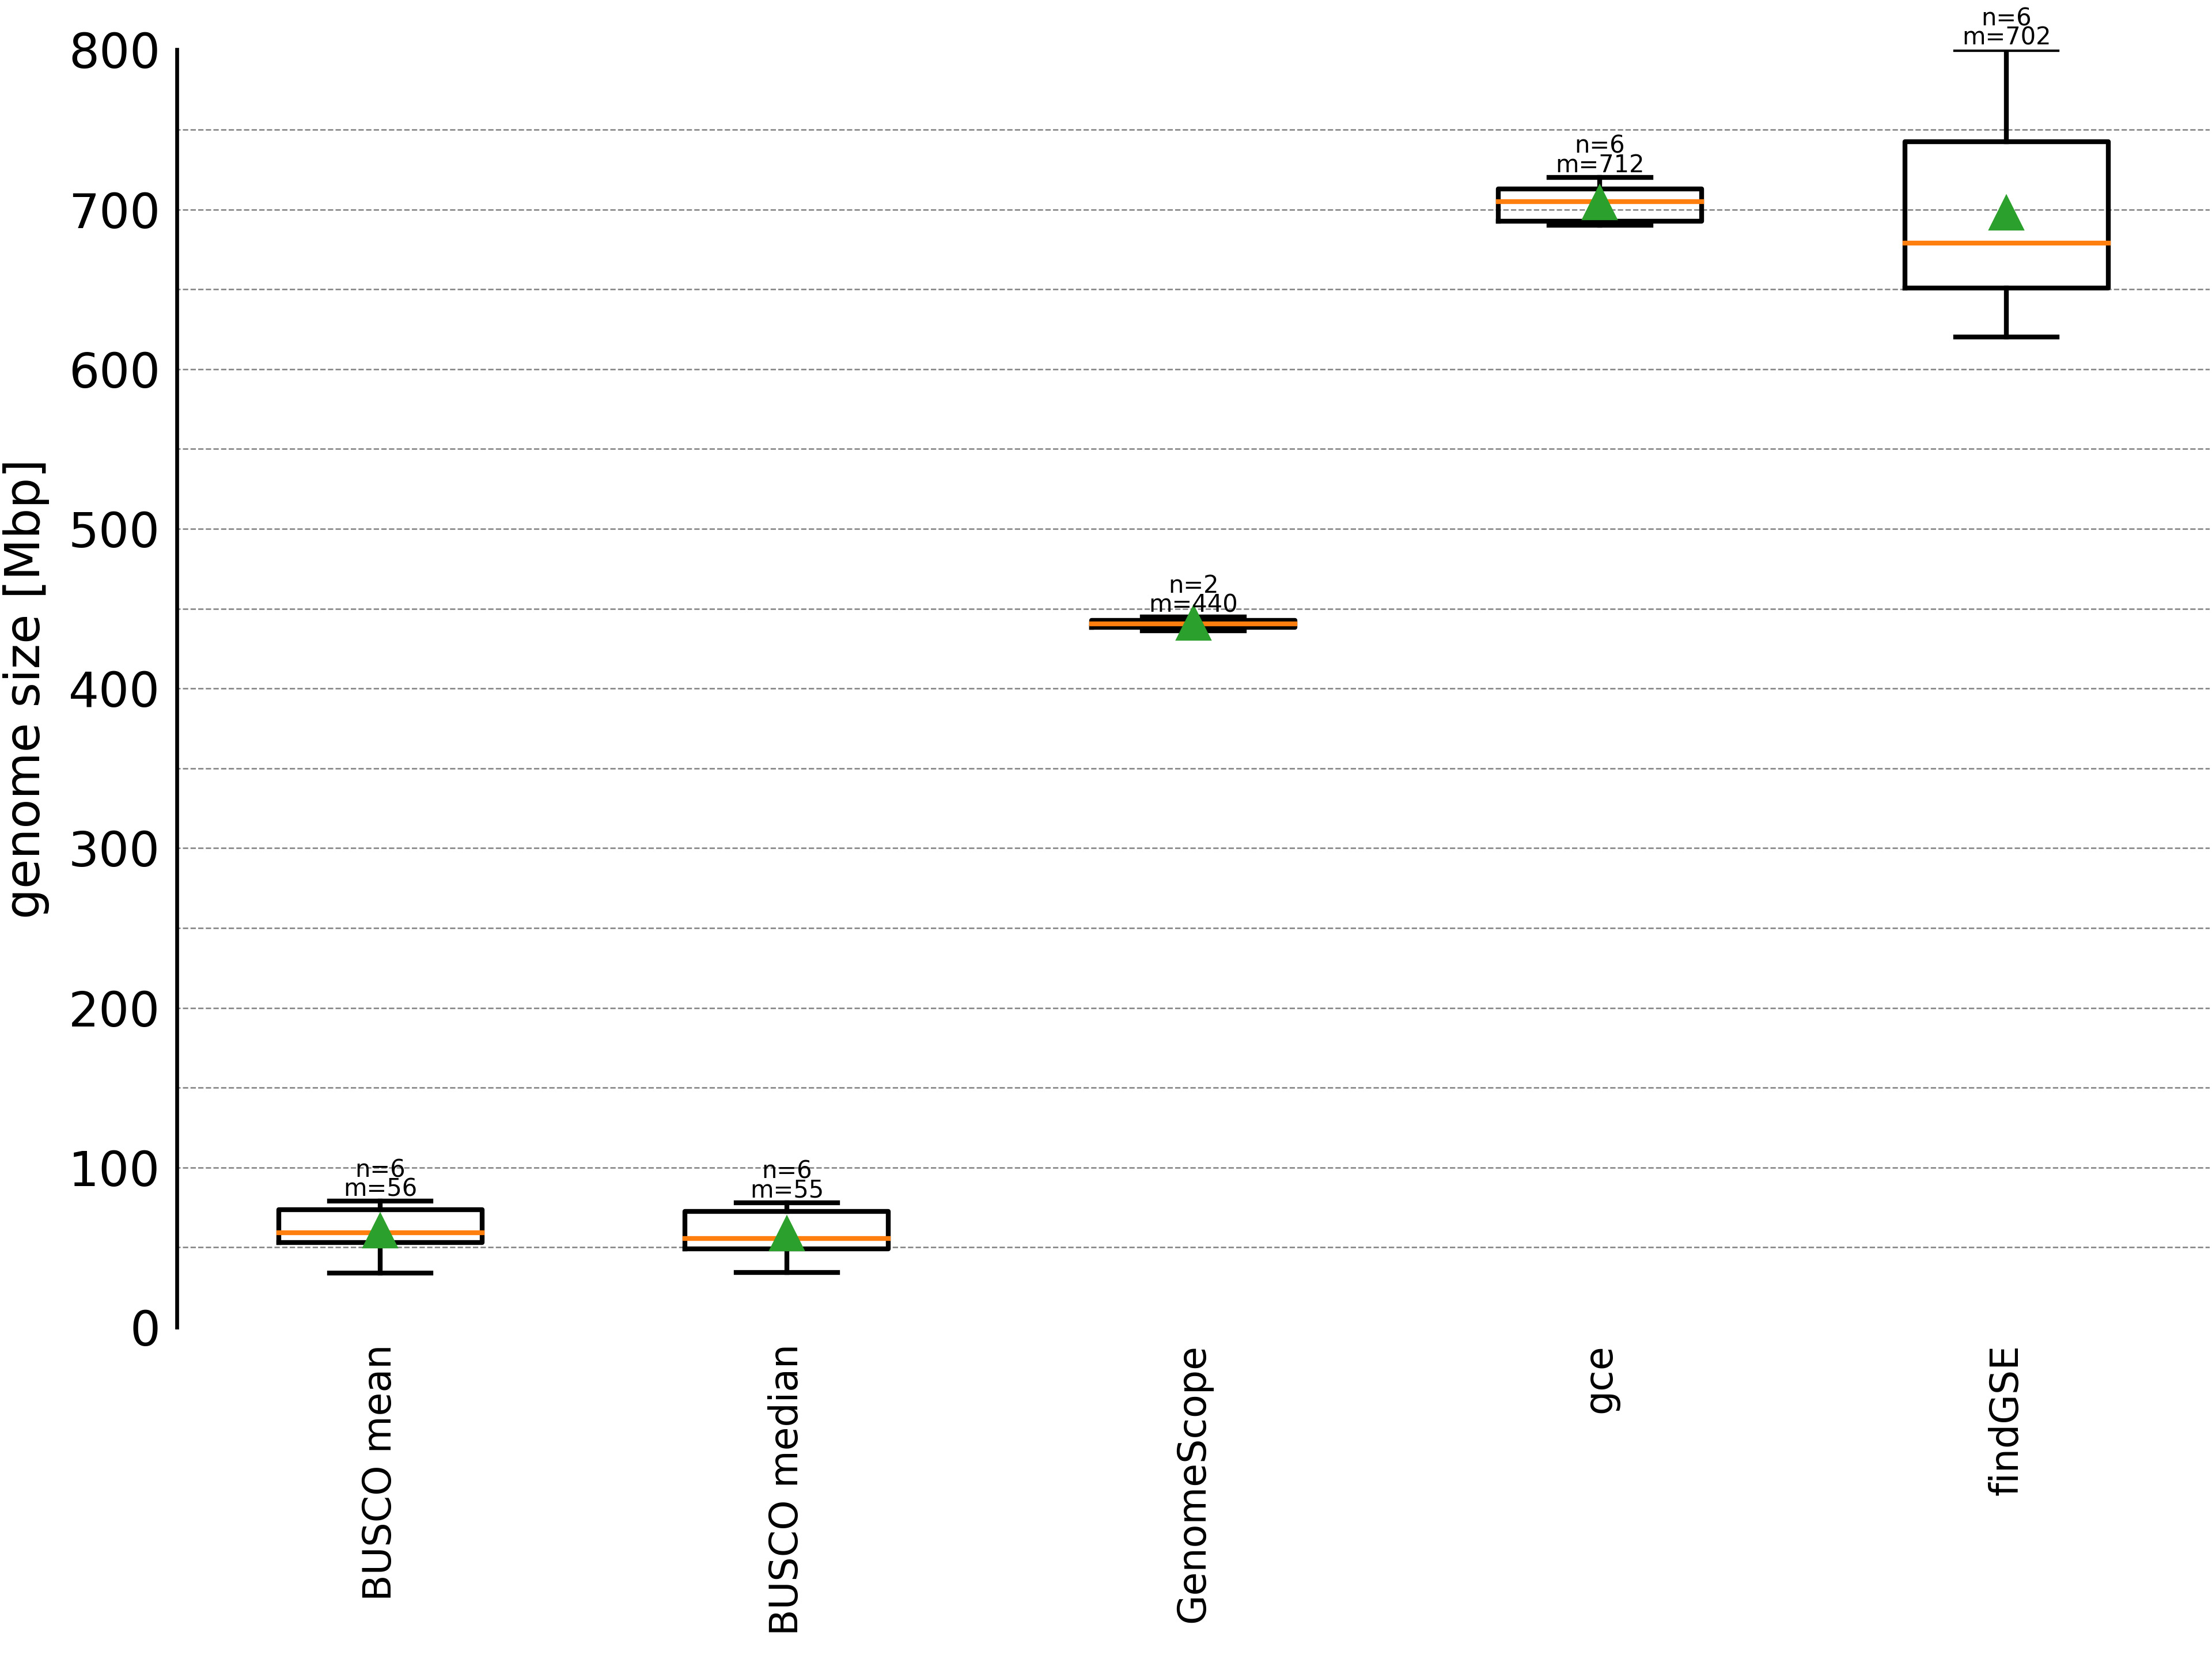
\includegraphics[width=0.45\textwidth]{capitoli/analisi/confronto/confronto2/9.jpg}}
		\caption{Dimensioni stimate dai metodi rispetto $n$ campioni di genomi di varie specie. Per il metodo MGSE vengono scelte la media o la mediana delle regioni BUSCO. La figura mostra per ogni stima il valor medio (in verde) e la mediana $m$ (in giallo).}
		\label{fig:2confronto5}
	\end{figure}
\end{document}
	
	\documentclass[crop=false, class=book]{standalone}

\begin{document}
	\chapter*{Conclusioni}
	\phantomsection
	\addcontentsline{toc}{chapter}{Conclusioni}	

	Il presente elaborato si è posto l'obiettivo di analizzare e confrontare i principali metodi di stima della dimensione del genoma tramite k-mer.
	
	Dopo una breve panoramica sui principali metodi di sequenziamento e di misurazione della dimensione del genoma attualmente disponibili, sono stati introdotti i k-mer e le loro principali proprietà. L'esposizione è quindi proseguita con l'analisi di ogni metodo, a partire dal punto di vista algoritmico e di gestione di casi particolari, fino alla valutazione della complessità e delle performance di ciascuno. Infine, l'analisi sperimentale dei risultati generati dai programmi ha permesso un confronto vero e proprio tra i metodi.
	
	Dall'analisi degli approcci basati sui k-mer emerge che il metodo ALLPATHS-LG risulta sovradimensionato per la sola stima della dimensione e poco preciso in situazioni particolari, come nel caso di bassa copertura o alto tasso di errore di sequenziamento; il programma GCE, inoltre, tende solitamente a sottostimare la dimensione del genoma. GenomeScope, pur riscontrando problemi nel caso di una copertura scarsa nelle letture di input, sembra essere un metodo di stima discreto. Infine, findGSE sembra possedere l'approccio più promettente, avendo anche un'alta correlazione con il metodo flow cytometry.
	
	Per quanto riguarda il programma MGSE, che presenta una complessità minore ma richiede informazioni più strutturate rispetto ai concorrenti, risulta un metodo efficiente nel caso di genomi di dimensioni ridotte. Infatti, la stima tramite la copertura ricavata dalle regioni BUSCO si dimostra precisa anche nei casi in cui altri metodi falliscono. Il programma, tuttavia, risulta poco accurato nell'analisi di genomi più particolari, come ad esempio un alto tasso di eterozigosi o un gran numero di \glspl{trasposone}. 
	
	Non esistendo attualmente un metodo affidabile che restituisca un valore di dimensione preciso per un genoma, risulta difficile determinare in modo assoluto il migliore tra i programmi trattati. In generale, si evince che alcuni metodi abbiano prestazioni migliori per certe tipologie di sequenze rispetto ad altri, ma che tutti riscontrino difficoltà nella trattazione di genomi di grandi dimensioni. 
	
	La stima della grandezza del genoma basata sui k-mer, assieme al metodo MGSE basato sull'individuazione di sequenze presenti in singola copia, comunque, anche grazie ai limitati requisiti richiesti, risultano essere approcci promettenti per lo sviluppo futuro di metodi più precisi ed efficienti.
	
	
	
\end{document}
	
	\backmatter
	\documentclass[crop=false]{standalone}

\begin{document}

	\printnoidxglossary[sort=word, style=list]

\end{document}
	
	\documentclass[crop=false]{standalone}

\usepackage[autostyle,italian=guillemets]{csquotes}
\usepackage[style=numeric,citestyle=numeric-comp,backend=biber]{biblatex}

\addbibresource{bibliografia.bib}

\begin{document}
	\printbibliography[heading=bibintoc]
\end{document}
	
	
\end{document}
